\documentclass[a4paper,12pt]{book}

\usepackage[T1,plmath]{polski}
\usepackage[utf8]{inputenc}
\usepackage{fancyhdr}
\usepackage{indentfirst}
\usepackage[pdftex]{graphicx}
\usepackage{amsfonts}
\usepackage{amsmath}
\usepackage{amssymb}
\usepackage{amsthm}
\usepackage[pdftex,
            left=1.1in,right=1.1in,
            top=1.1in,bottom=1.1in]{geometry}
\usepackage{float}
\usepackage[section]{placeins}
\usepackage[font=small,labelfont=bf]{caption}
\usepackage{cite}
\usepackage{listings}
\usepackage{xcolor}
\usepackage{tikz}
\usetikzlibrary{arrows.meta, positioning, decorations.pathreplacing}
\usepackage{booktabs}
\usepackage[ruled,linesnumbered,noend,algochapter]{algorithm2e}
\SetKwFor{ForEach}{dla każdej cząstki}{wykonaj}{}
\SetKwFor{ForAllJ}{dla każdego sąsiada}{wykonaj}{}
\usepackage[colorlinks=true]{hyperref}
\hypersetup{allcolors=black}

\lstset{
    basicstyle=\footnotesize\ttfamily,
    numbers=left,
    numberstyle=\tiny,
    frame=tb,
    tabsize=4,
    columns=fixed,
    showstringspaces=false,
    keepspaces,
    commentstyle=\color{red},
    keywordstyle=\color{blue},
    extendedchars=true,
    inputencoding=utf8,
    literate={ą}{{\k{a}}}1 {ć}{{\'c}}1 {ę}{{\k{e}}}1 {ł}{{\l}}1 {ń}{{\'n}}1 {ó}{{\'o}}1 {ś}{{\'s}}1 {ź}{{\'z}}1 {ż}{{\.z}}1
             {Ą}{{\k{A}}}1 {Ć}{{\'C}}1 {Ę}{{\k{E}}}1 {Ł}{{\L}}1 {Ń}{{\'N}}1 {Ó}{{\'O}}1 {Ś}{{\'S}}1 {Ź}{{\'Z}}1 {Ż}{{\.Z}}1,
    captionpos=b
}

\pagestyle{fancy}
\renewcommand{\chaptermark}[1]{\markboth{#1}{}}
\renewcommand{\sectionmark}[1]{\markright{\thesection\ #1}}
\fancyhf{}
\fancyhead[LE,RO]{\footnotesize\bfseries\thepage}
\fancyhead[LO]{\footnotesize\rightmark}
\fancyhead[RE]{\footnotesize\leftmark}
\renewcommand{\headrulewidth}{0.5pt}
\addtolength{\headheight}{1.5pt}
\fancypagestyle{plain}{\fancyhead{}\cfoot{\footnotesize\bfseries\thepage}\renewcommand{\headrulewidth}{0pt}}

\linespread{1.25}
\bibliographystyle{plain}

\begin{document}

% --------------------
% Tytułowa strona (titlepage.tex)
% --------------------
\begin{titlepage}
\noindent
\begin{tabular}{c@{\hspace{21mm}}|@{\hspace{5mm}}l}
\vspace{-20mm} & \\
\multicolumn{2}{l}{\hspace{-12.5mm} 
\includegraphics[width=8cm]{logo-umcs.jpg}} \\
\multicolumn{2}{@{\hspace{20mm}}l}{\vspace{-4mm}} \\
\multicolumn{2}{@{\hspace{28mm}}l}{\Large \sf UNIWERSYTET MARII CURIE-SKŁODOWSKIEJ} \\
\multicolumn{2}{@{\hspace{28mm}}l}{\vspace{-4mm}} \\
\multicolumn{2}{@{\hspace{28mm}}l}{\Large \sf W LUBLINIE} \\
\multicolumn{2}{@{\hspace{28mm}}l}{\vspace{-4mm}} \\
\multicolumn{2}{@{\hspace{28mm}}l}{\Large \sf Wydział Matematyki, Fizyki i Informatyki} \\
\multicolumn{2}{@{\hspace{28mm}}l}{\vspace{21mm}} \\
& {\sf Kierunek: \textbf{Informatyka}} \\
& \\\\\\
& {\sf \large \bfseries Nikita Lysiuk} \\
& {\sf nr albumu: 320828} \\
& \\\\\\
& \Large \sf \bfseries Symulacja i wizualizacja cieczy w czasie \\
& \Large \sf \bfseries rzeczywistym za pomocą Rust i Vulkan API \\[10pt]
& {\large \sf Real-Time Fluid Simulation and Visualization} \\
& {\large \sf using Rust and the Vulkan API} \\
& \\
& \\
& \\
& {\sf Praca licencjacka}  \\
& \vspace{-7mm} \\
& {\sf napisana w Katedrze ...} \\ % Upewnij się co do nazwy katedry
& {\sf Instytutu Informatyki UMCS} \\
& \vspace{-7mm} \\
& {\sf pod kierunkiem \bfseries (stopień/tytuł, imię i nazwisko promotora)} \\
\multicolumn{2}{@{\hspace{28mm}}l}{\vspace{15mm}} \\
\multicolumn{2}{@{\hspace{28mm}}l}{\textbf{\textsf{Lublin 2026}}}
\end{tabular}
\end{titlepage}
\cleardoublepage

\thispagestyle{empty}
\newpage

\tableofcontents
\cleardoublepage

\chapter*{Wstęp}
\addcontentsline{toc}{chapter}{Wstęp}
\chaptermark{Wstęp}
Realistyczne odwzorowanie zachowania cieczy od lat pozostaje jednym
z~najbardziej wymagających zadań grafiki komputerowej. Woda towarzyszy
człowiekowi na co dzień, dlatego widz natychmiast dostrzega każde uproszczenie:
nienaturalny rozprysk, brak załamania światła czy zbyt gładką powierzchnię fali.
Jednocześnie zapotrzebowanie na wiarygodne symulacje płynów stale rośnie ---
od produkcji filmowej i~gier komputerowych, przez wizualizacje naukowe,
po inżynierskie analizy przepływów. W~produkcji offline, gdzie pojedyncza klatka
może powstawać godzinami, jakość symulacji ogranicza wyłącznie budżet
obliczeniowy; w~zastosowaniach interaktywnych ograniczenie jest znacznie
bardziej rygorystyczne, ponieważ pełny krok fizyki wraz z~renderowaniem musi
zmieścić się w~kilkunastu milisekundach.

Spełnienie tego wymagania stało się możliwe dzięki ewolucji procesorów
graficznych, które z~wyspecjalizowanych układów rasteryzujących przekształciły
się w~masowo równoległe maszyny obliczeniowe ogólnego przeznaczenia.
Współczesne GPU wykonuje jednocześnie dziesiątki tysięcy wątków, co naturalnie
odpowiada strukturze symulacji cząsteczkowych, w~których ten sam zestaw operacji
stosowany jest niezależnie do każdego elementu cieczy. Pełne wykorzystanie tego
potencjału wymaga jednak narzędzi dających programiście bezpośrednią kontrolę
nad sprzętem: niskopoziomowych API graficznych oraz języków systemowych
łączących wydajność z~gwarancjami poprawności. Tymczasem dojrzałe systemy
symulacji cieczy --- zarówno pakiety animacyjne, jak i~biblioteki badawcze ---
wykonują centralne obliczenia w~przeważającej mierze na procesorze głównym,
a~obecność karty graficznej wykorzystują głównie do wyświetlania wyników.

Celem niniejszej pracy jest zaprojektowanie i~implementacja interaktywnego
silnika symulacji cieczy, w~którym kompletny potok obliczeniowy --- od dynamiki
cząstek, przez wymuszanie nieściśliwości, po wolumetryczną wizualizację ---
wykonywany jest w~czasie rzeczywistym w~całości na procesorze graficznym.
Fundament fizyczny systemu stanowi cząsteczkowa metoda SPH w~wariancie DFSPH,
wymuszającym nieściśliwość cieczy przez dwuetapową korekcję gęstości
i~dywergencji pola prędkości. Warstwę technologiczną tworzą język programowania
Rust oraz niskopoziomowe API graficzne Vulkan --- połączenie oferujące
statyczne bezpieczeństwo pamięci przy zachowaniu jawnej kontroli nad zasobami
sprzętowymi. Zakres pracy obejmuje sformułowanie podstaw teoretycznych metody
SPH i~algorytmu DFSPH, uzasadniony dobór stosu technologicznego, implementację
solvera oraz potoku wizualizacji wraz z~autorskimi rozwiązaniami
architektonicznymi, a~także ilościową analizę wydajności i~zbieżności
zaimplementowanych algorytmów.

Praca składa się z~trzech rozdziałów. W~rozdziale pierwszym przedstawiono
podstawy teoretyczne: porównanie eulerowskiego i~lagrange'owskiego opisu ruchu
płynów, równania Naviera-Stokesa, dyskretyzację jądrową metody SPH wraz
z~algorytmem DFSPH oraz koncepcję wolumetrycznej wizualizacji metodą przemarszu
promienia. Rozdział drugi zawiera przegląd istniejących rozwiązań symulacji
cieczy oraz charakterystykę wybranych technologii: języka Rust, API Vulkan
i~biblioteki Vulkano, narzędzi diagnostycznych, a~ponadto analizę porównawczą
funkcji wygładzających, struktur wyszukiwania sąsiedztwa i~modeli zjawisk
fizycznych. Rozdział trzeci dokumentuje implementację systemu: architekturę
aplikacji, organizację danych w~pamięci GPU, potok wyszukiwania sąsiadów wraz
z~porównaniem dwóch algorytmów sortowania, kolejne etapy solvera DFSPH oraz
potok renderowania --- każdorazowo z~uzasadnieniem podjętych decyzji
i~pomiarami wydajności. Pracę zamyka podsumowanie zestawiające osiągnięte
rezultaty oraz kierunki dalszego rozwoju systemu.

\cleardoublepage

% 5. Розділи основної частини
\chapter{Metodyka i podstawy teoretyczne symulacji i wizualizacji cieczy}
\section{Porównanie podejścia Lagrange'owskiego i Eulerowskiego}

Ciecze stanowią jedno z najbardziej fascynujących, a zarazem złożonych zjawisk fizycznych, symulacja których pozostaje wyzwaniem dla współczesnej informatyki i fizyki obliczeniowej. Historia matematycznego opisu ich ruchu sięga XVIII wieku i wiąże się z pracami dwóch pionierów nowożytnej analizy: Leonharda Eulera oraz Josepha Louisa Lagrange'a. Wypracowane przez nich koncepcje teoretyczne stanowią fundament, na którym opierają się wszystkie dzisiejsze techniki cyfrowej rekonstrukcji dynamiki płynów.

Pierwsze udane próby numerycznego rozwiązania pełnych równań Naviera-Stokesa dla cieczy o swobodnej powierzchni datuje się na rok 1965. Wówczas Francis Harlow i J. Eddie Welch z Los Alamos National Laboratory zaproponowali metodę \textit{marker and cell} (MAC)\cite{harlow1965numerical}. Rozwiązanie to oparto na podejściu eulerowskim, w którym parametry fizyczne analizowane są w ustalonych punktach przestrzeni, tworzących regularną strukturę geometryczną. Chociaż algorytmy siatkowe ewoluowały i są z sukcesami stosowane do dziś, charakteryzują się one istotnymi ograniczeniami, zwłaszcza w obliczu gwałtownych zjawisk takich jak silne rozpryski czy szybkie zmiany topologii powierzchni cieczy.

W odpowiedzi na te trudności, w 1977 roku środowisko astrofizyków zaproponowało alternatywną koncepcję --- \textit{smoothed particle hydrodynamics} (SPH)\cite{gingold1977smoothed}. Metoda ta czerpie bezpośrednią inspirację z lagrange'owskiego opisu materii, traktując ciecz jako zbiór dyskretnych elementów masy swobodnie przemieszczających się w przestrzeni. Od czasu publikacji prac Gingolda i Monaghana, technika SPH doczekała się licznych wariantów optymalizacyjnych, stając się jednym z najchętniej wybieranych narzędzi w grafice komputerowej czasu rzeczywistego.

Analizując oba podejścia, należy zauważyć, że każde z nich oferuje unikalny zestaw zalet i wad. Metody siatkowe gwarantują wysoką stabilność numeryczną i precyzję obliczeń gradientów ciśnienia. Z kolei metody cząsteczkowe cechują się naturalnym zachowaniem masy oraz brakiem ograniczeń co do rozmiaru domeny obliczeniowej. Współczesne dążenie do maksymalizacji realizmu przy jednoczesnym zachowaniu wydajności doprowadziło do powstania metod hybrydowych, takich jak FLIP (\textit{fluid-implicit particle}) \cite{brackbill1986flip}. Stały się one de facto standardem w przemyśle filmowym oraz mediach interaktywnych, łącząc stabilność siatki eulerowskiej z elastycznością cząsteczek lagrange'owskich. Rozwiązania te, choć niezwykle skuteczne, wykraczają poza zakres niniejszej pracy. Skupia się ona na czystym sformułowaniu cząsteczkowym jako rozwiązaniu najlepiej wykorzystującym architekturę nowoczesnych procesorów graficznych.

\subsection{Istota podejścia Eulerowskiego}
Podejście Eulerowskie, którego fundamenty położył Leonhard Euler w połowie XVIII wieku \cite{euler1757principes, euler1761principia}, stanowi jeden z dwóch głównych sposobów opisu ruchu materii w mechanice kontinuum. W przeciwieństwie do śledzenia pojedynczych cząstek, koncepcja ta skupia się na stałych punktach w przestrzeni, przez które przepływa płyn. Zamiast pytać „gdzie przemieścił się dany element cieczy?”, analizujemy pytanie „jaka jest prędkość i ciśnienie w tym konkretnym miejscu w danym momencie?” \cite{braley2010fluid}. Matematycznie podejście to opiera się na analizie pól fizycznych. Zmiana dowolnej właściwości płynu $Q$ (np. gęstości lub prędkości) jest opisywana przez tzw. pochodną materiałową, która pozwala połączyć obserwację w stałym punkcie z faktem, że płyn jest w ruchu:
\begin{equation}
\frac{DQ}{Dt} = \frac{\partial Q}{\partial t} + \mathbf{u} \cdot \nabla Q
\end{equation}

Wzór ten pokazuje, że całkowita zmiana wartości wynika z dwóch czynników: lokalnej zmiany w czasie ($\frac{\partial Q}{\partial t}$) oraz efektu transportu tej wartości przez poruszający się płyn ($\mathbf{u} \cdot \nabla Q$). Współczesne techniki komputerowe, opierając się na tych założeniach, wykorzystują metody siatkowe. Jak wspomniano wcześniej, pionierami tego rozwiązania byli Francis Harlow i J. Eddie Welch, którzy w 1965 roku wprowadzili metodę MAC\cite{harlow1965numerical}. Ich kluczowym pomysłem było nałożenie na przestrzeń nieruchomej, regularnej siatki obliczeniowej. W takim modelu parametry płynu są obliczane tylko w węzłach lub na ściankach komórek tej siatki, co pozwala na numeryczne rozwiązanie skomplikowanych równań ruchu. Podejście oparte na siatce posiada charakterystyczny zestaw cech:\begin{itemize}
\item \textbf{Zalety:} Główną mocną stroną jest wysoka precyzja matematyczna i stabilność obliczeń. Stała struktura siatki ułatwia wyznaczanie różnic w ciśnieniu, co jest kluczowe dla zachowania realizmu w symulacjach płynów o dużej objętości (np. dymu czy spokojnej wody).
\item \textbf{Wady:} Największym wyzwaniem jest tzw. dyfuzja numeryczna, czyli nienaturalne "rozmywanie się" detali płynu podczas jego przemieszczania się między komórkami. Ponadto, siatki mają trudności z dokładnym śledzeniem swobodnej powierzchni cieczy. Wymaga to stosowania dodatkowych, kosztownych technik śledzenia powierzchni, takich jak \textit{metoda poziomic} (ang. \textit{Level-Set}) lub \textit{metoda śledzenia objętości} (ang. \textit{Volume of Fluid}), które przy gwałtownych ruchach i rozpryskach tracą drobne szczegóły, takie jak pojedyncze krople.\end{itemize}

Podsumowując, podejście Eulerowskie jest niezwykle skuteczne tam, gdzie płyn wypełnia całą dostępną przestrzeń, jednak staje się mniej wydajne w scenariuszach wymagających symulacji dynamicznych rozprysków i szybkich zmian kształtu cieczy.

\subsection{Istota podejścia Lagrange'owskiego}
Podejście Lagrange'owskie, sformułowane przez Josepha Louisa de Lagrange'a w jego fundamentalnych pracach nad teorią ruchu płynów \cite{lagrange1788mecanique}, oferuje zgoła odmienną perspektywę obserwacji materii niż model eulerowski. Zamiast analizować zmiany parametrów w stałych punktach przestrzeni, badacz podąża za konkretnym elementem masy wzdłuż jego trajektorii. W tym ujęciu współrzędne każdego punktu cieczy są funkcjami czasu oraz ich pozycji początkowej, co pozwala na bezpośrednie śledzenie historii ruchu poszczególnych fragmentów materii.

Matematycznie ruch w opisie lagrange'owskim wyraża się poprzez funkcję mapowania $\mathbf{x} = \chi(\mathbf{X}, t)$, gdzie $\mathbf{X}$ to pozycja referencyjna cząstki w chwili początkowej, a $\mathbf{x}$ to jej aktualne położenie. Kluczową cechą tej metody jest naturalne zachowanie masy oraz uproszczenie równań adwekcji, które w tym modelu stają się tożsame z ruchem samej cząstki. Pozwala to na uniknięcie problemu dyfuzji numerycznej, będącej największą słabością metod siatkowych, oraz umożliwia modelowanie zjawisk o nieskończonym zasięgu bez konieczności definiowania sztywnej domeny obliczeniowej.

Mimo solidnych fundamentów matematycznych, praktyczne zastosowanie tego podejścia do złożonych symulacji cieczy pojawiło się dopiero w 1977 roku wraz z metodą \textit{smoothed particle hydrodynamics} (SPH) \cite{gingold1977smoothed}. Motywacja do jej stworzenia płynęła z potrzeb astrofizyki – badacze tacy jak Gingold i Monaghan poszukiwali sposobu na modelowanie dynamicznych układów gwiazdowych i procesów formowania się galaktyk, gdzie materia ulega ekstremalnym deformacjom i przemieszczeniom w próżni. Tradycyjne metody oparte na siatce okazywały się całkowicie niewydolne w symulowaniu obiektów, które nie posiadają stałych granic i swobodnie ewoluują w otwartej przestrzeni.

Wprowadzenie SPH jako alternatywy dla metod siatkowych było zatem podyktowane koniecznością obsłużenia scenariuszy, w których topologia płynu zmienia się w sposób gwałtowny i nieprzewidywalny. Główne charakterystyki tego podejścia obejmują:\begin{itemize}\item \textbf{Zalety:} Największym atutem jest brak konieczności stosowania skomplikowanych algorytmów śledzenia powierzchni. Ciecz jest definiowana przez samą obecność cząstek, co sprawia, że tworzenie się kropel, łączenie fal czy rozpryski są efektem ubocznym fizyki cząsteczkowej, a nie dodatkowym zadaniem geometrycznym.\item \textbf{Wady:} Podejście to wprowadza nowe wyzwania obliczeniowe, z których najistotniejszym jest brak stałych relacji między elementami. W każdym kroku symulacji konieczne jest ponowne wyznaczanie sąsiedztwa cząstek, co wymaga zaawansowanych struktur danych. Ponadto, uzyskanie stabilności ciśnienia jest w tym modelu znacznie trudniejsze niż na regularnej siatce, co doprowadziło do powstania złożonych wariantów algorytmu, takich jak DFSPH czy PBF.\end{itemize}

Podsumowując, podejście Lagrange'owskie przekształca problem dynamiki cieczy z analizy pól w analizę oddziaływań między elementami dyskretnymi. Jest to koncepcja, która mimo większego skomplikowania w zakresie optymalizacji struktur danych, oferuje niezrównaną elastyczność w wizualizacji dynamicznych i silnie rozproszonych zjawisk wodnych.


\section{Sformułowanie matematyczne metody cząsteczkowej SPH i jej wariantu DFSPH}
W celu przejścia od modelu ciągłego do postaci obliczeniowej konieczne jest sformułowanie równań Naviera–Stokesa w sposób umożliwiający ich dyskretyzację w ramach metody cząsteczkowej.
\subsection{ Równania Naviera-Stokesa jako fundament teoretyczny} 
Zarówno metody siatkowe, jak i bezsiatkowe (takie jak SPH), stanowią numeryczne przybliżenia rozwiązań układu różniczkowych równań cząstkowych, nazwanego na cześć Claude'a-Louisa Naviera oraz Sir George'a Gabriela Stokesa. Prace nad tymi równaniami, prowadzone w latach 1822–1850, zdefiniowały sposób, w jaki współczesna fizyka opisuje ruch płynów lepkich \cite{batchelor1967introduction}. Każda analiza z zakresu symulacji cieczy musi opierać się na tym fundamencie, który de facto stanowi sformułowanie podstawowych praw zachowania masy i pędu w mechanice kontinuum \cite{mclean2012continuum}.

Pełny opis dynamiki cieczy wymaga spełnienia dwóch kluczowych warunków:
\begin{enumerate}
\item Zachowanie masy (Równanie ciągłości):
Równanie to opisuje relację między gęstością cieczy a jej przepływem. W formie lagrange'owskiej przyjmuje ono postać:
\begin{equation}
\frac{D\rho}{Dt} = -\rho \nabla \cdot \mathbf{u}
\end{equation}
Informuje ono, że zmiana gęstości elementu masy jest bezpośrednio związana z dywergencją pola prędkości ($\nabla \cdot \mathbf{u}$). W przypadku cieczy nieściśliwych, gęstość powinna pozostać stała ($\frac{D\rho}{Dt} = 0$), co wymusza bezdywergencyjny charakter pola prędkości.

\item Zachowanie pędu (Równanie Cauchy’ego):
Opisuje zachowanie ośrodka ciągłego pod wpływem działających na niego sił \cite{landau1987fluid}:
    \begin{equation}
        \rho \frac{D\mathbf{u}}{Dt} = -\nabla p + \nabla \cdot \mathbf{\tau} + \rho \mathbf{a}
    \end{equation}Gdzie poszczególne symbole oznaczają:
    \begin{itemize}
        \item $\frac{D}{Dt}$ – pochodna materiałowa (operator $\frac{\partial}{\partial t} + \mathbf{u} \cdot \nabla$), łącząca zmianę lokalną z efektem adwekcji,
        \item $\rho$ – gęstość masy cieczy,\item $\mathbf{u}$ – wektor prędkości przepływu,\item $p$ – ciśnienie izotropowe (składowa determinująca siłę ciśnienia),
        \item $\mathbf{\tau}$ – tensor naprężeń dewiacyjnych (odpowiedzialny za opór lepki),
        \item $\mathbf{a}$ – przyspieszenia masowe (np. grawitacja $\mathbf{g}$).
    \end{itemize}
\end{enumerate}

W kontekście niniejszej pracy, równania te dostarczają ramy analitycznej dla algorytmu SPH. Pokazują one, że ruch cieczy jest wynikiem bilansu sił: wewnętrznego gradientu ciśnienia (powstającego w odpowiedzi na zmiany gęstości), oporu wynikającego z lepkości oraz oddziaływań zewnętrznych. To właśnie sprzężenie między równaniem ciągłości a równaniem pędu pozwala wyznaczyć ciśnienie $p$, które koryguje prędkości cząsteczek tak, aby zachować stałą objętość cieczy. Zadaniem metody SPH jest przekształcenie tych ciągłych zależności w dyskretne interakcje między punktami masy.

\subsection{Interpolacja jądrowa i dyskretyzacja SPH}
Istota metody SPH polega na śledzeniu właściwości fizycznych cieczy poprzez analizę dyskretnych punktów masy. Fundamentem tej techniki jest matematyczna koncepcja dystrybucji Diraca $\delta$ oraz powiązana z nią tożsamość Diraca. W ujęciu idealnym, cząsteczkę można traktować jako nieskończenie mały punkt, w którym cała siła skupiona jest w jednym miejscu, a poza nim wynosi zero:
\begin{equation}
    \delta(r) = \begin{cases} \infty & \text{jeśli } r = 0 \\ 0 & \text{w przeciwnym razie} \end{cases}
\end{equation}

Dodatkowo, musi zostać spełniony warunek normalizacji, oznaczający, że niezależnie od wybranego obszaru całkowania, masa całkowita pozostaje jednostkowa: 

\begin{equation}
    \int \delta(r) dv = 1
\end{equation}


W rzeczywistości komputerowej bezpośrednia implementacja nieskończenie małych punktów nie jest możliwa ze względu na ograniczoną precyzję maszynową oraz konieczność operowania na skończonych zbiorach danych. Niezbędny jest zatem sposób na dyskretyzację tych założeń. Rozwiązaniem jest wprowadzenie funkcji jądra  (lub~funkcji~wygładzającej) $W$. Jej rolą jest "rozmycie" właściwości cząsteczki z punktu do obszaru o określonym promieniu oddziaływania $h$. Gradient tej funkcji opisuje nie tylko siłę wpływu sąsiednich cząsteczek, ale także kierunek zmian tych oddziaływań \cite{koschier2020smoothed}.

Dzięki temu dowolną właściwość fizyczną $A(\mathbf{x})$ możemy przybliżyć poprzez splot z funkcją jądra:
\begin{equation}
    A(\mathbf{x}) \approx (A * W)(\mathbf{x}) = \int A(\mathbf{x}') W(\mathbf{x} - \mathbf{x}', h) d\mathbf{x}'
\end{equation}

Ponieważ system komputerowy operuje na skończonej pamięci, nie możemy rozważać całki po bezgranicznej przestrzeni. W procesie dyskretyzacji całka zostaje zastąpiona sumą po skończonej liczbie sąsiadujących cząsteczek \cite{mon92}:
\begin{equation}
    \langle A(\mathbf{x}_i) \rangle \approx \sum_j \frac{m_j}{\rho_j} A(\mathbf{x}_j) W(\mathbf{x}_i - \mathbf{x}_j, h)
\end{equation}

Aby funkcja jądra była użyteczna w stabilnej symulacji cieczy, musi spełniać szereg rygorystycznych warunków matematycznych \cite{koschier2020smoothed}:
\begin{itemize}
    \item \textbf{Warunek normalizacji:} $\int W(r', h) dv' = 1$, co gwarantuje zachowanie całkowitej wartości przybliżanej wielkości.
    \item \textbf{Warunek Diraca:} $\lim_{h \to 0} W(r, h) = \delta(r)$, co oznacza, że wraz ze zmniejszaniem promienia $h$, przybliżenie dąży do rozwiązania idealnego.
    \item \textbf{Dodatniość i symetria:} $W(r, h) \ge 0$ oraz $W(r, h) = W(-r, h)$.
    \item \textbf{Zwarta podpora:} $W(r, h) = 0$ dla $r \ge h$. Jest to kluczowy warunek z punktu widzenia wydajności — komputer musi analizować tylko te cząsteczki, które znajdują się w fizycznym zasięgu oddziaływania, co drastycznie redukuje liczbę operacji.
\end{itemize}

Praktycznym przykładem zastosowania tej teorii jest obliczanie gęstości $\rho_i$ dla wybranej cząsteczki. Stosując powyższą dyskretyzację, otrzymujemy sumę mas sąsiadów ważoną funkcją jądra:
\begin{equation}
    \rho_i = \sum_{j} m_j W(\mathbf{x}_i - \mathbf{x}_j, h)
\end{equation}

W tym przypadku gęstość w mianowniku wzoru ogólnego redukuje się, pozostawiając prostą zależność od masy, co pozwala na efektywne obliczanie lokalnego zagęszczenia cieczy przy skończonych zasobach obliczeniowych.

\subsection{Algorytm Divergence-Free SPH (DFSPH)}

Mimo że klasyczne sformułowanie SPH pozwala na wizualnie atrakcyjne symulacje, boryka się ono z problemem wysokiej ściśliwości cieczy oraz niestabilnością przy większych krokach czasowych. Tradycyjne rozwiązania, oparte na równaniach stanu (EOS), wymagają bardzo małych wartości $\Delta t$, aby uniknąć „zapadania się” objętości cieczy. Rozwiązaniem tych problemów jest algorytm Divergence-Free Smoothed Particle Hydrodynamics, zaproponowany przez Jana Bendera i Dana Koschiera \cite{bender2015divergence}.

Istota DFSPH sprowadza się do rygorystycznego wymuszenia nieściśliwości poprzez iteracyjne rozwiązanie dyskretnego układu równań wynikających z warunku nieściśliwości z różnymi wyrazami źródłowymi. Podejście to pozwala na stabilizację cieczy na dwóch poziomach:
\begin{enumerate}
    \item Poziom zagęszczenia: Celem tego etapu jest utrzymanie stałej objętości cieczy poprzez korekcję pozycji cząsteczek. Algorytm wyznacza błąd gęstości, biorąc pod uwagę różnicę między gęstością bieżącą a spoczynkową $\rho_0$, a następnie uwzględnia wpływ zmian prędkości wynikających z adwekcji. Logiczną strukturę tego procesu opisuje poniższy pseudokod:
    \begin{lstlisting}[caption={Algorytm wyznaczania wyrazu źródłowego gęstości}, label={alg:density_source}]
        Dla każdej cząsteczki i:
        1. Pobierz bieżącą gęstość rho_i oraz gęstość docelową rho_0.
        2. Oblicz sumę dywergencji na podstawie różnic 
        prędkości między i oraz sąsiadami j.
        3. Wyznacz błąd gęstości w czasie: 
           source = ((rho_0 - rho_i) / delta_t) - suma_dywergencji
        4. Zapisz wyraz źródłowy do obliczeń sił ciśnienia.
    \end{lstlisting}
    \item Poziom prędkości: Nawet po skorygowaniu gęstości, pole prędkości może zawierać błędy, które w kolejnym kroku czasowym spowodowałyby ponowne zagęszczenie materii. Drugi solver działa wyłącznie na wektorach prędkości, eliminując ich zbieżność lub rozbieżność:
       \begin{lstlisting}[caption={Algorytm wyznaczania wyrazu źródłowego dywergencji}, label={alg:div_source}]
        Dla każdej cząsteczki i:
        1. Zainicjalizuj sumę dywergencji jako 0.
        2. Dla każdego sąsiada j:
           a. Oblicz różnicę prędkości (v_i - v_j).
           b. Pomnóż różnicę przez gradient funkcji jądra.
           c. Dodaj wynik (ważony masą) do sumy.
        3. Wyznacz wyraz źródłowy jako negację sumy dywergencji:
           source = -suma_dywergencji
    \end{lstlisting}
\end{enumerate}

Wybór algorytmu DFSPH jest kluczowy dla systemów pracujących w czasie rzeczywistym. Dzięki dwuetapowej korekcji, metoda ta jest znacznie bardziej odporna na błędy numeryczne niż popularne alternatywy, takie jak PBF (Position Based Fluids) czy IISPH (Implicit Incompressible SPH).

Główną zaletą DFSPH jest możliwość stosowania znacznie większego kroku czasowego $\Delta t$ bez ryzyka "eksplozji" symulacji. Przekłada się to bezpośrednio na całkowity czas obliczeń potrzebny do wygenerowania sekwencji ruchu. Poniższa tabela porównuje wydajność DFSPH z innymi metodami, wskazując na jej dominację w scenariuszach wymagających szybkości.

\begin{table}[ht]
    \centering
    \small
    \begin{tabular}{lcccc}
    \toprule
    $\Delta t$ [ms] & IISPH [s] & PBF [s] & PCISPH [s] & \textbf{DFSPH [s]} \\ \midrule
    4.0             & 318.1     & 613.5   & 1085.7     & 51.3                \\
    2.0             & 267.9     & 508.4   & 1021.2     & 59.4                 \\
    1.0             & 220.7     & 338.0   & 656.9      & 107.5                 \\
    0.5             & 225.6     & 240.5   & 394.9      & 210.8                  \\
    0.25            & 402.2     & 354.0   & 440.9      & 372.0                   \\ \bottomrule
    \end{tabular}
    \caption{Porównanie całkowitego czasu obliczeń dla różnych metod SPH 
    \cite{bender2015divergence}}
    \label{tab:performance_comparison}
\end{table}

Przedstawione sformułowanie matematyczne metody SPH oraz algorytmu DFSPH definiuje fizyczny fundament systemu. Dzięki dyskretyzacji kontinuum cieczy za pomocą chmury punktów oraz rygorystycznemu wymuszeniu nieściśliwości przez dwuetapowy solver ciśnienia, możliwe jest uzyskanie stabilnej i wydajnej symulacji w czasie rzeczywistym.

Jednak wynik symulacji w czystej postaci Lagrange’owskiej to jedynie zbiór danych o pozycjach i prędkościach cząsteczek — surowa „chmura punktów”, która nie posiada wizualnych cech ciągłej cieczy, takich jak gładka powierzchnia, załamania światła czy przezroczystość. Aby przekształcić te dane w realistyczny obraz, konieczne jest zastosowanie zaawansowanych technik graficznych.

\section{Wizualizacja objętościowa metodą Ray Marching}
Przekształcenie surowych danych cząsteczkowych, pochodzących z symulacji SPH, w ciągły i fotorealistyczny obraz cieczy wymaga zastosowania metod pośredniej reprezentacji materii. W przeciwieństwie do klasycznych technik graficznych, które opierają się na generowaniu jawnej geometrii, w niniejszej pracy zdecydowano się na wykorzystanie bezpośredniego renderowania objętościowego. Koncepcja ta, zaproponowana przez Marca Levoya \cite{levoy1988volume}, zakłada formowanie obrazu bezpośrednio z danych wolumetrycznych bez konieczności kosztownej ekstrakcji izopowierzchni do postaci siatki wielokątów. Proces ten składa się z dwóch głównych etapów:
\begin{itemize}
    \item Rekonstrukcja ciągłego pola skalarnego: Symulacja w ujęciu lagrange’owskim dostarcza jedynie dyskretny zbiór punktów masowych. Aby umożliwić analizę wizualną cieczy jako obiektu ciągłego, konieczne jest odtworzenie pola gęstości w każdym punkcie przestrzeni symulacji. Wykorzystuje się do tego znaną z matematycznego sformułowania SPH tożsamość interpolacyjną:
    \begin{equation}
        \rho(\mathbf{x}) = \sum_{j} m_j W(|\mathbf{x} - \mathbf{x}_j|, h)
    \end{equation}
    
    Gdzie $\mathbf{x}$ jest dowolnym punktem w przestrzeni, a $W$ funkcją wygładzającą. Równanie to opisuje przejście od punktowej reprezentacji materii do trójwymiarowego, ciągłego pola objętościowego, spopularyzowanego w nowoczesnej grafice czasu rzeczywistego m.in. przez prace Inigo Quileza \cite{quilez2008raymarching}. W praktyce obliczeniowej pole to poddawane jest dyskretyzacji — przestrzeń symulacji dzieli się na regularną strukturę o rozdzielczości $N_x \times N_y \times N_z$, gdzie każdy węzeł przechowuje próbkowaną wartość gęstości $\rho_{i,j,k} = \rho(\mathbf{x}_{i,j,k})$.
    
    \item Numeryczna integracja promieni: Głównym narzędziem wizualizacji tak przygotowanego pola jest algorytm Ray Marching. Jest to metoda numerycznej integracji światła przechodzącego przez ośrodek objętościowy, która dzięki pełnej paralelizacji idealnie nadaje się do realizacji w środowisku GPU \cite{tomczak2012gpu}. W modelu tym dla każdego piksela obrazu generowany jest promień rzutujący:
    \begin{equation}
        \mathbf{r}(t) = \mathbf{o} + t\mathbf{d}
    \end{equation}
    Gdzie $\mathbf{o}$ to punkt obserwacji (kamera), a $\mathbf{d}$ to wektor kierunku promienia. Promień ten „kroczy” przez pole objętościowe w małych krokach $\Delta t$, a w każdym punkcie $\mathbf{x}_k = \mathbf{o} + k\Delta t \mathbf{d}$ następuje próbkowanie gęstości.

    Wizualizacja opiera się na przybliżeniu całki objętościowej, która określa końcowy kolor piksela na podstawie lokalnej absorpcji i transmisji światła w cieczy. Kluczową zaletą tego podejścia w kontekście wydajności jest fakt, że proces ten odbywa się całkowicie w przestrzeni ekranu, zazwyczaj wewnątrz shaderów fragmentów. Oznacza to, że system nie buduje fizycznej siatki wielokątów, lecz dynamicznie wyznacza punkty przecięcia promienia z izopowierzchnią cieczy\cite{quilez2013advancing}.
\end{itemize}

Aby umożliwić realistyczne oświetlenie cieczy (obliczanie odbić i załamań światła), konieczne jest wyznaczenie wektora normalnego do jej powierzchni. Ponieważ powierzchnia w renderingu objętościowym nie jest zdefiniowana wprost, wektor normalny $\mathbf{n}$ aproksymuje się jako znormalizowany gradient pola gęstości:
\begin{equation}
    \mathbf{n} = \frac{\nabla \rho}{|\nabla \rho|}
\end{equation}

Gradient ten wskazuje kierunek najszybszego wzrostu gęstości, co pozwala matematycznie traktować granice obszarów o wysokiej gęstości jako fizyczną barierę cieczy. Dzięki temu możliwe jest zastosowanie klasycznych modeli oświetlenia, takich jak model Phonga, oraz zaawansowanych efektów optycznych wynikających z praw Snella i Fresnela\cite{de2006reflections}.

Zastosowanie rekonstrukcji objętościowej i algorytmu Ray Marching stanowi pomost między dyskretnymi danymi fizycznymi a ciągłym obrazem. Pozwala to na uzyskanie wysokiej jakości wizualizacji z naturalnie wyglądającymi detalami powierzchni, zachowując jednocześnie wysoką wydajność obliczeniową na nowoczesnych układach graficznych.

Przedstawione w niniejszym rozdziale podstawy teoretyczne — od eulerowskiego i lagrange'owskiego opisu ruchu, przez sformułowanie metody SPH, aż po techniki bezpośredniego renderowania objętościowego — definiują ramy matematyczne niezbędne do budowy kompletnego systemu symulacji. Jednak transformacja tych abstrakcyjnych modeli w działającą aplikację czasu rzeczywistego wymaga starannego doboru stosu technologicznego. Wybór odpowiedniego języka programowania, interfejsów programowania aplikacji graficznych oraz struktur danych ma kluczowy wpływ na ostateczną wydajność i stabilność systemu. W kolejnym rozdziale dokonano przeglądu technologii oraz środowiska programistycznego, które umożliwiły implementację opisanych mechanizmów z wykorzystaniem pełnej mocy obliczeniowej współczesnych procesorów i układów graficznych. 

\chapter{Przegląd technologii i środowisko programistyczne}

Przedstawione w poprzednim rozdziale podstawy teoretyczne --- od eulerowskiego i
lagrange'owskiego opisu ruchu, przez sformułowanie metody SPH, aż po techniki bezpośredniego
renderowania objętościowego --- definiują ramy matematyczne niezbędne do budowy kompletnego systemu symulacji.
Jednak transformacja tych abstrakcyjnych modeli w działającą aplikację czasu rzeczywistego wymaga starannego
doboru stosu technologicznego. Wybór odpowiedniego języka programowania, interfejsów programowania aplikacji
graficznych oraz struktur danych ma kluczowy wpływ na ostateczną wydajność i stabilność systemu.
W niniejszym rozdziale dokonano przeglądu technologii oraz środowiska programistycznego, które umożliwiły
implementację opisanych mechanizmów z wykorzystaniem pełnej mocy obliczeniowej współczesnych procesorów
i układów graficznych.

\section{Istniejące rozwiązania symulacji cieczy}

Współczesne techniki symulacji cieczy ewoluowały w stronę metod hybrydowych oraz optymalizowanych 
podejść cząsteczkowych, aby sprostać wymaganiom realizmu w nauce i rozrywce. Współczesne rozwiązania
obejmują szeroki wachlarz podejść --- od metod czysto eulerowskich i czysto cząsteczkowych po hybrydy obu. 
Jak omówiono w rozdziale pierwszym, aktualnym standardem przemysłowym jest metoda FLIP, łącząca stabilność 
siatki eulerowskiej z elastycznością cząsteczek lagrange'owskich \cite{brackbill1986flip}. 
Dominuje ona w silnikach przeznaczonych do tworzenia gier i animacji, gdzie liczy się zarówno wydajność, 
jak i jakość wizualna.

Obok rozwiązań opartych na FLIP istnieje jednak ekosystem narzędzi skoncentrowanych wyłącznie 
na formułowaniu cząsteczkowym SPH. Szczególne miejsce zajmuje tu biblioteka SPlisHSPlasH, 
tworzona przez tę samą grupę badawczą, która zaproponowała algorytm DFSPH będący przedmiotem 
niniejszej pracy \cite{SPlisHSPlasH_Library, bender2015divergence}. 
Przegląd reprezentatywnych narzędzi z obu obszarów pozwala uchwycić różnorodność 
podejść projektowych oraz wyznaczyć punkt, w którym lokuje się system opisany w dalszej części pracy.

\subsection{Symulacja FLIP w programie Blender}

Blender jest wolnym i otwartoźródłowym pakietem do modelowania, animacji i~renderowania 
trójwymiarowego, rozwijanym przez Blender Foundation od 1994 roku \cite{blender2023}. 
Narzędzia symulacji cieczy dostępne w tym programie opierają się na silniku Mantaflow, 
zintegrowanym z Blenderem począwszy od wersji 2.82 \cite{mantaflow2021}. 
Implementacja ta korzysta z metody FLIP, w której domenę obliczeniową opisuje siatka 
eulerowska, a~cząsteczki lagrange'owskie pełnią rolę tracerów adwekcji ---
znaczników śledzących, które przenoszą prędkość przepływu między kolejnymi krokami symulacji. 
Centralna logika obliczeniowa wykonywana jest na procesorze głównym.

Blender jest narzędziem zorientowanym na fizycznie dokładną animację komputerową --- jego 
narzędzia symulacyjne nie stawiają sobie za cel pracy w czasie rzeczywistym, 
lecz maksymalną jakość wyników. Narzędzie zaprojektowano z myślą o generowaniu sekwencji animacji, 
w których jakość fizyczna i wizualna stawiana jest ponad ograniczeniami czasu rzeczywistego. 
Wynik symulacji jest zapisywany na dysku jako pamięć podręczna danych wolumetrycznych, a następnie 
renderowany niezależnie za pomocą rendererów Cycles lub EEVEE. Podejście to sprawdza się doskonale w 
produkcji filmowej i reklamowej, lecz ze swej natury wyklucza interaktywność i sprzężenie zwrotne w czasie 
rzeczywistym. Typowy widok interfejsu konfiguracji domeny i podglądu pola cieczy przedstawia rysunek~\ref{fig:blender_flip}.

\begin{figure}[ht]
    \centering
    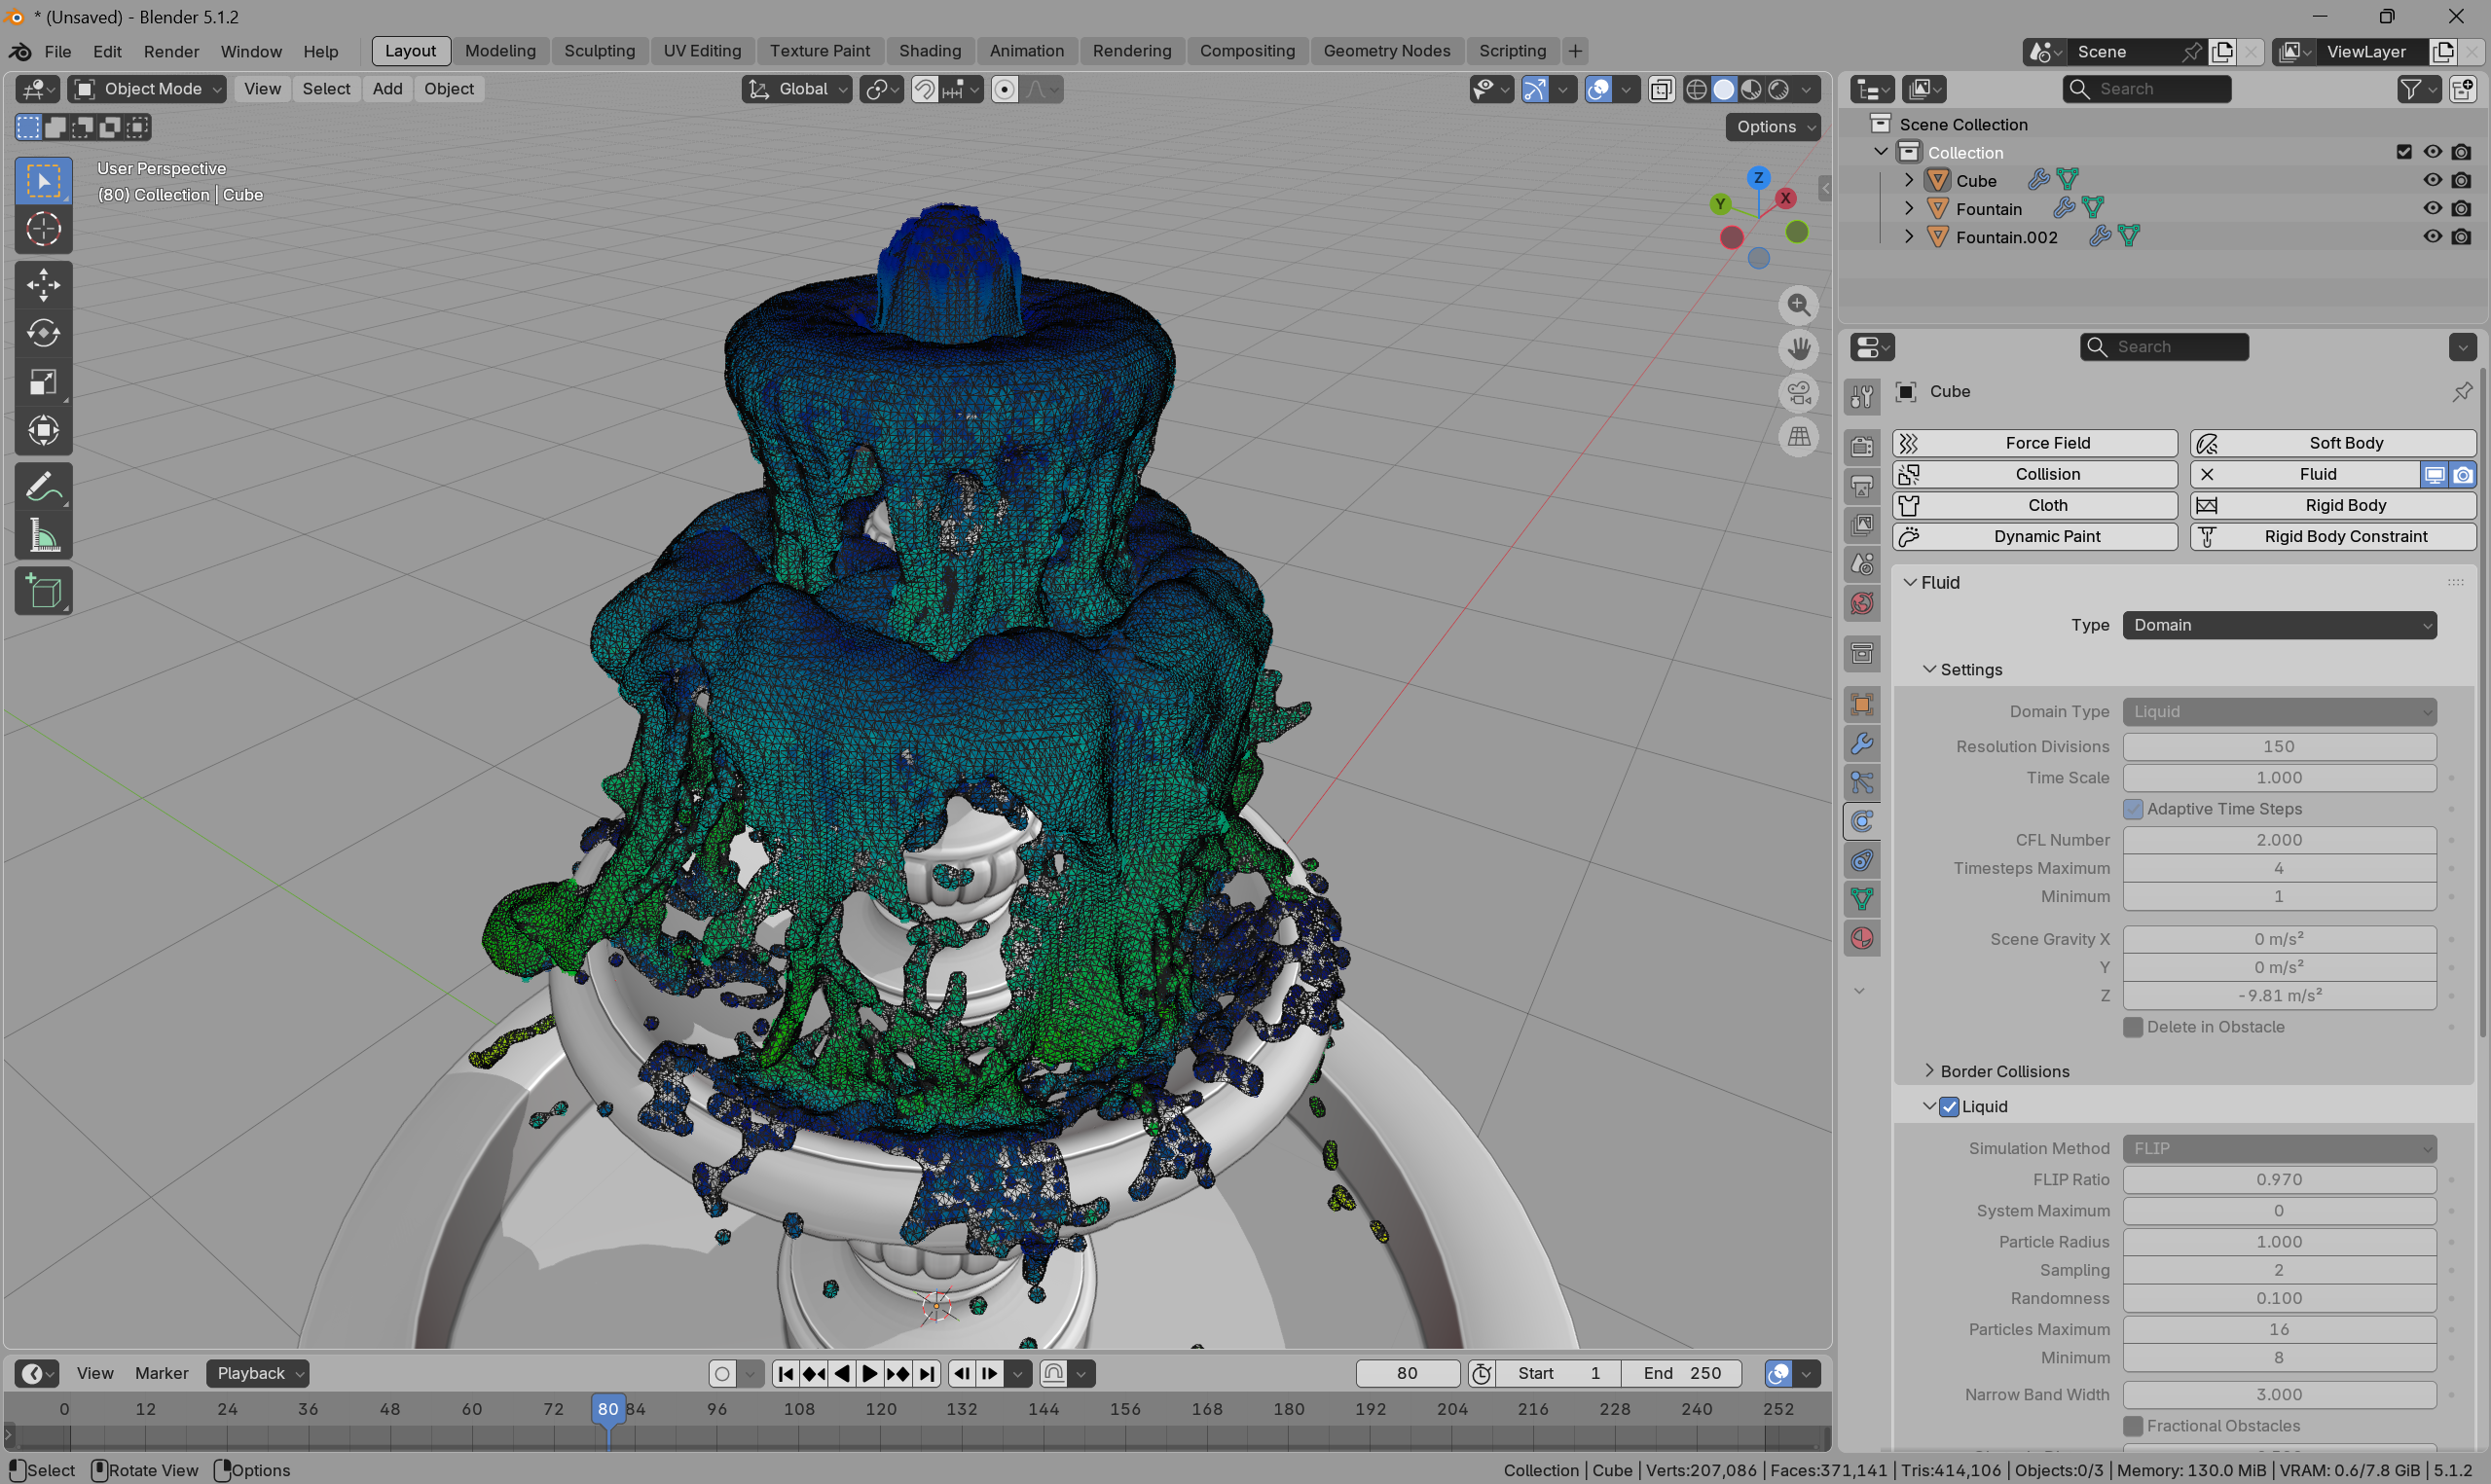
\includegraphics[width=0.85\textwidth]{figures/blender_flip.png}
    \caption{Interfejs symulacji FLIP w programie Blender z widocznym panelem konfiguracji domeny i podglądem cieczy \newline Źródło: Własne opracowanie na podstawie dokumentacji \cite{blenderdocs2023}}
    \label{fig:blender_flip}
\end{figure}

\subsection{Symulacja FLIP w silniku Unreal Engine 5}

Unreal Engine 5 jest zaawansowanym silnikiem aplikacji interaktywnych, rozwijanym przez Epic Games i 
stosowanym zarówno w produkcji gier, jak i przy tworzeniu efektów wizualnych dla filmów i symulacji \cite{ue5fluids}. 
Jednym z jego kluczowych podsystemów jest Niagara --- elastyczny system efektów wizualnych i cząsteczkowych, 
wykonujący obliczenia w całości na GPU. Możliwości symulacji cieczy udostępnia wtyczka NiagaraFluids, 
implementująca metodę FLIP dla trójwymiarowych cieczy.

Środowisko pracy oparte jest na edytorze węzłów, widocznym na rysunku~\ref{fig:ue5_flip}, 
który oferuje gotowe szablony symulacji przeznaczone do bezpośredniego umieszczenia na poziomie gry. 
Szablony te stanowią punkt wyjścia do dalszej personalizacji --- modularna architektura komponentów pozwala twórcy dostosować 
każdy aspekt symulacji do konkretnego zadania, od konfiguracji sił i warunków brzegowych, aż po modyfikację 
poszczególnych kroków solvera. Silnik jest zatem rozwiązaniem skalowalnym: 
umożliwia zarówno szybkie składanie efektów przez artystów --- osoby bez specjalistycznego
przygotowania programistycznego, konfigurujące symulację wyłącznie przez interfejs graficzny ---
jak i głębszą ingerencję algorytmiczną przez programistów efektów, którzy mają możliwość pisania
własnych modułów obliczeniowych i modyfikowania wewnętrznej logiki solvera.

\begin{figure}[ht]
    \centering
    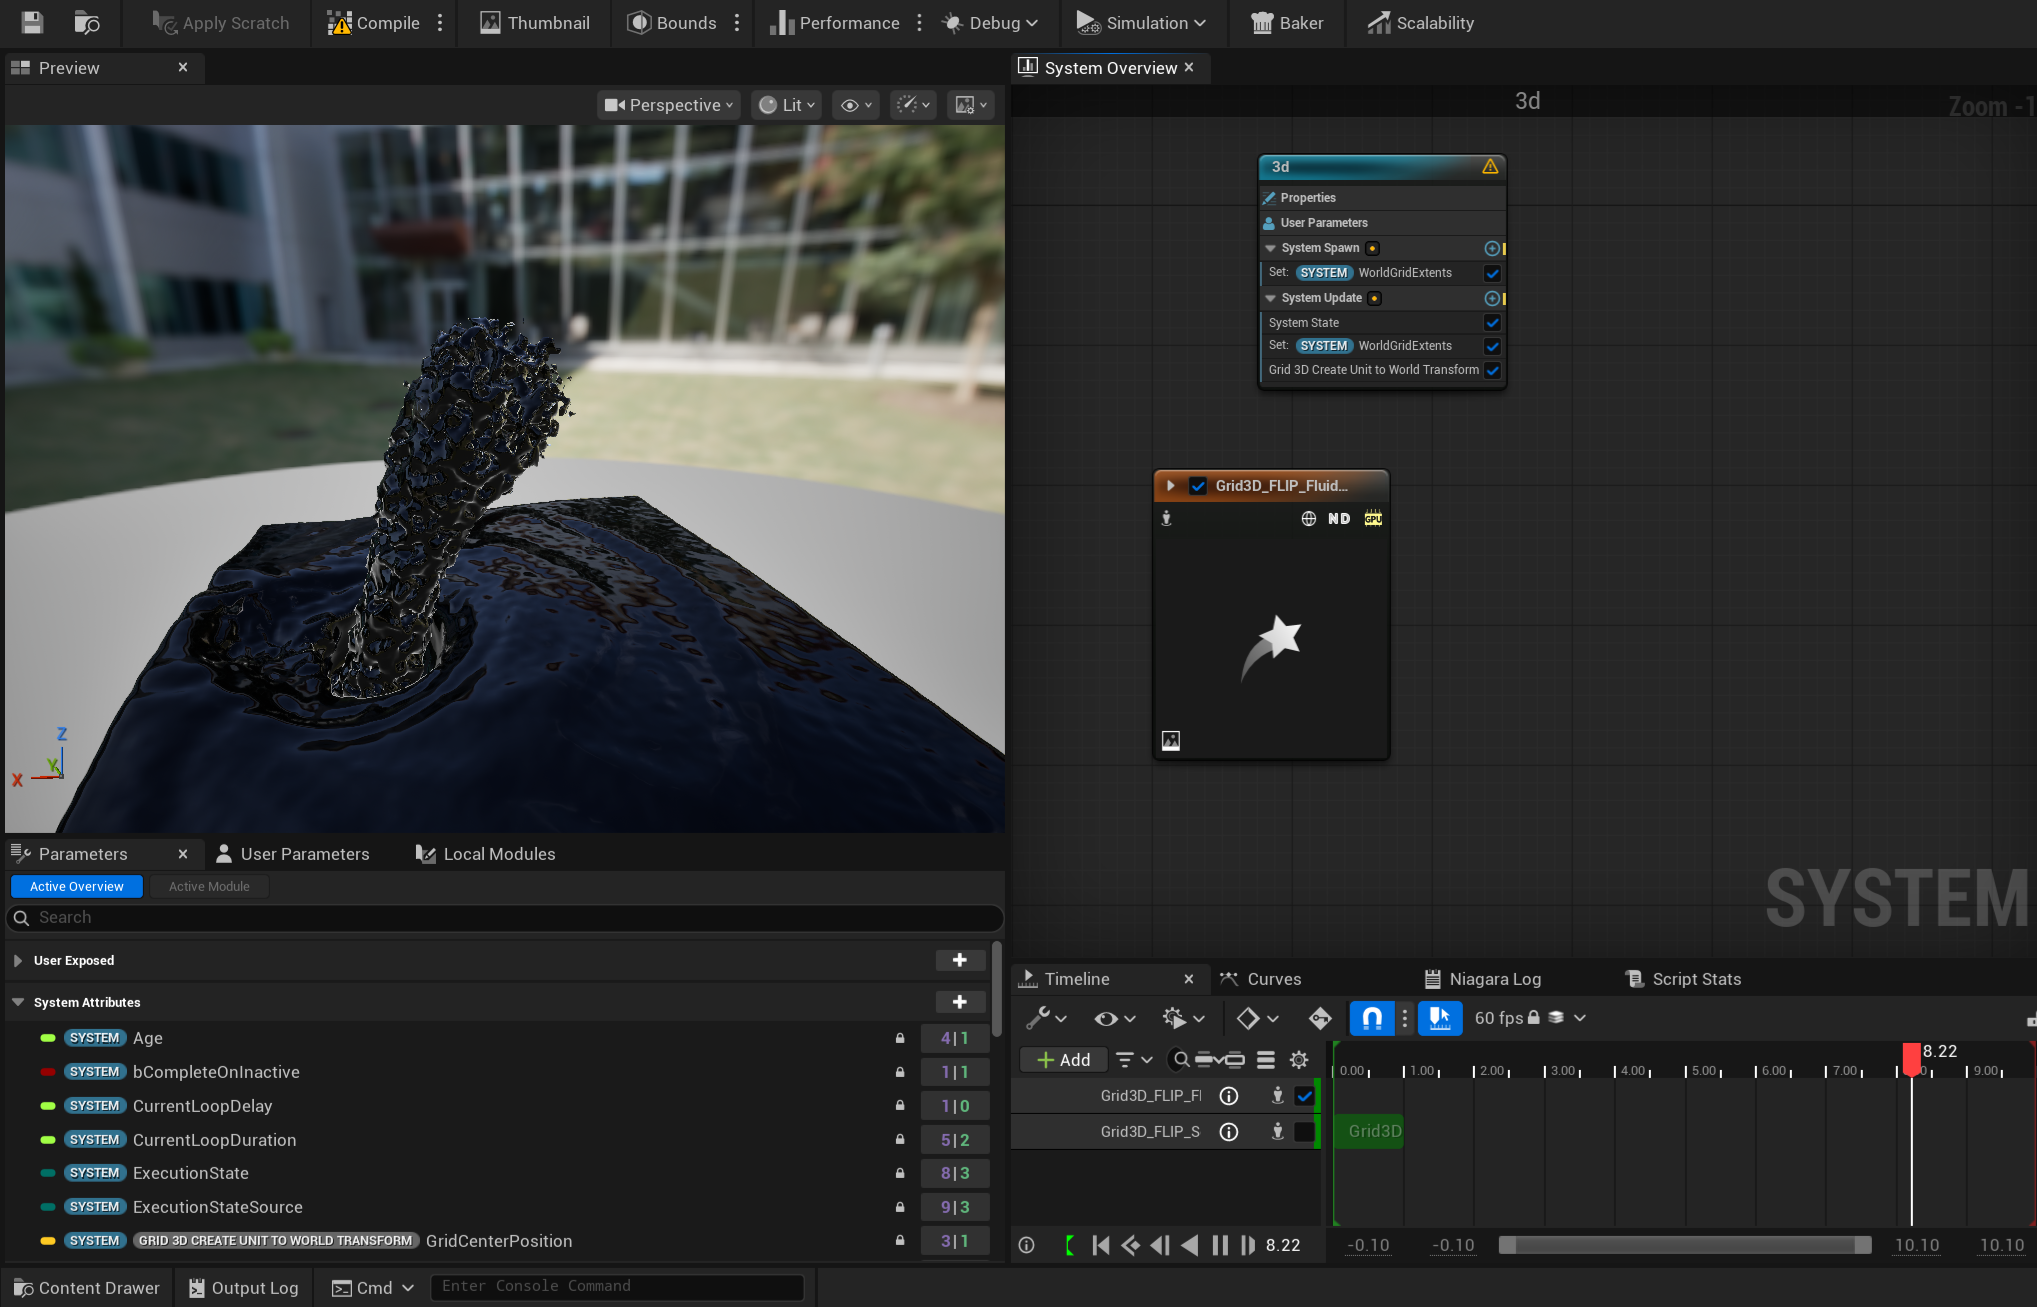
\includegraphics[width=0.85\textwidth]{figures/ue5_flip.png}
    \caption{Interfejs edytora Niagara w silniku Unreal Engine 5 z aktywną symulacją 3D FLIP zrealizowaną przy użyciu wtyczki NiagaraFluids \newline Źródło: Własne opracowanie na podstawie dokumentacji \cite{ue5fluids}}
    \label{fig:ue5_flip}
\end{figure}

\subsection{Biblioteka SPlisHSPlasH}

SPlisHSPlasH (ang.~\textit{Smoothed Particle Hydrodynamics Simulation Library}) jest 
otwartą biblioteką symulacyjną tworzoną przez grupę badawczą Jana Bendera \cite{SPlisHSPlasH_Library}. 
W odróżnieniu od dwóch poprzednich rozwiązań, biblioteka ta opiera się wyłącznie na metodzie SPH w 
formie cząsteczkowej, bez stosowania pomocniczej siatki eulerowskiej. Pod względem przyjętego modelu 
fizycznego stanowi ona najbliższy odpowiednik systemu opisanego w niniejszej pracy.

Biblioteka implementuje zestaw nowoczesnych solverów nieściśliwości, w tym m.in. DFSPH. 
Ponadto wspierane są modele fenomenologiczne lepkości, napięcia powierzchniowego i sił wirowania. 
Jej architektura opiera się wyłącznie na języku C++, a cały potok symulacyjny wykonywany jest na procesorze głównym. 
Jedynym krokiem dopuszczającym opcjonalne przeniesienie obliczeń na GPU jest wyszukiwanie sąsiedztwa, 
realizowane przez zewnętrzną bibliotekę Compact\-N\-Search --- jej wariant cu\-N\-Search umożliwia wykonanie tego 
kroku na karcie graficznej \cite{CompactNSearch_Library}. Warstwa wizualizacyjna 
korzysta z OpenGL~3.3 wyłącznie do renderowania wyników symulacji, co widoczne jest na rysunku~\ref{fig:splishsplash}. 
SPlisHSPlasH jest szeroko stosowana w środowisku naukowym jako platforma referencyjna do testowania i 
porównywania nowych algorytmów SPH \cite{koschier2020smoothed}.

\begin{figure}[ht]
    \centering
    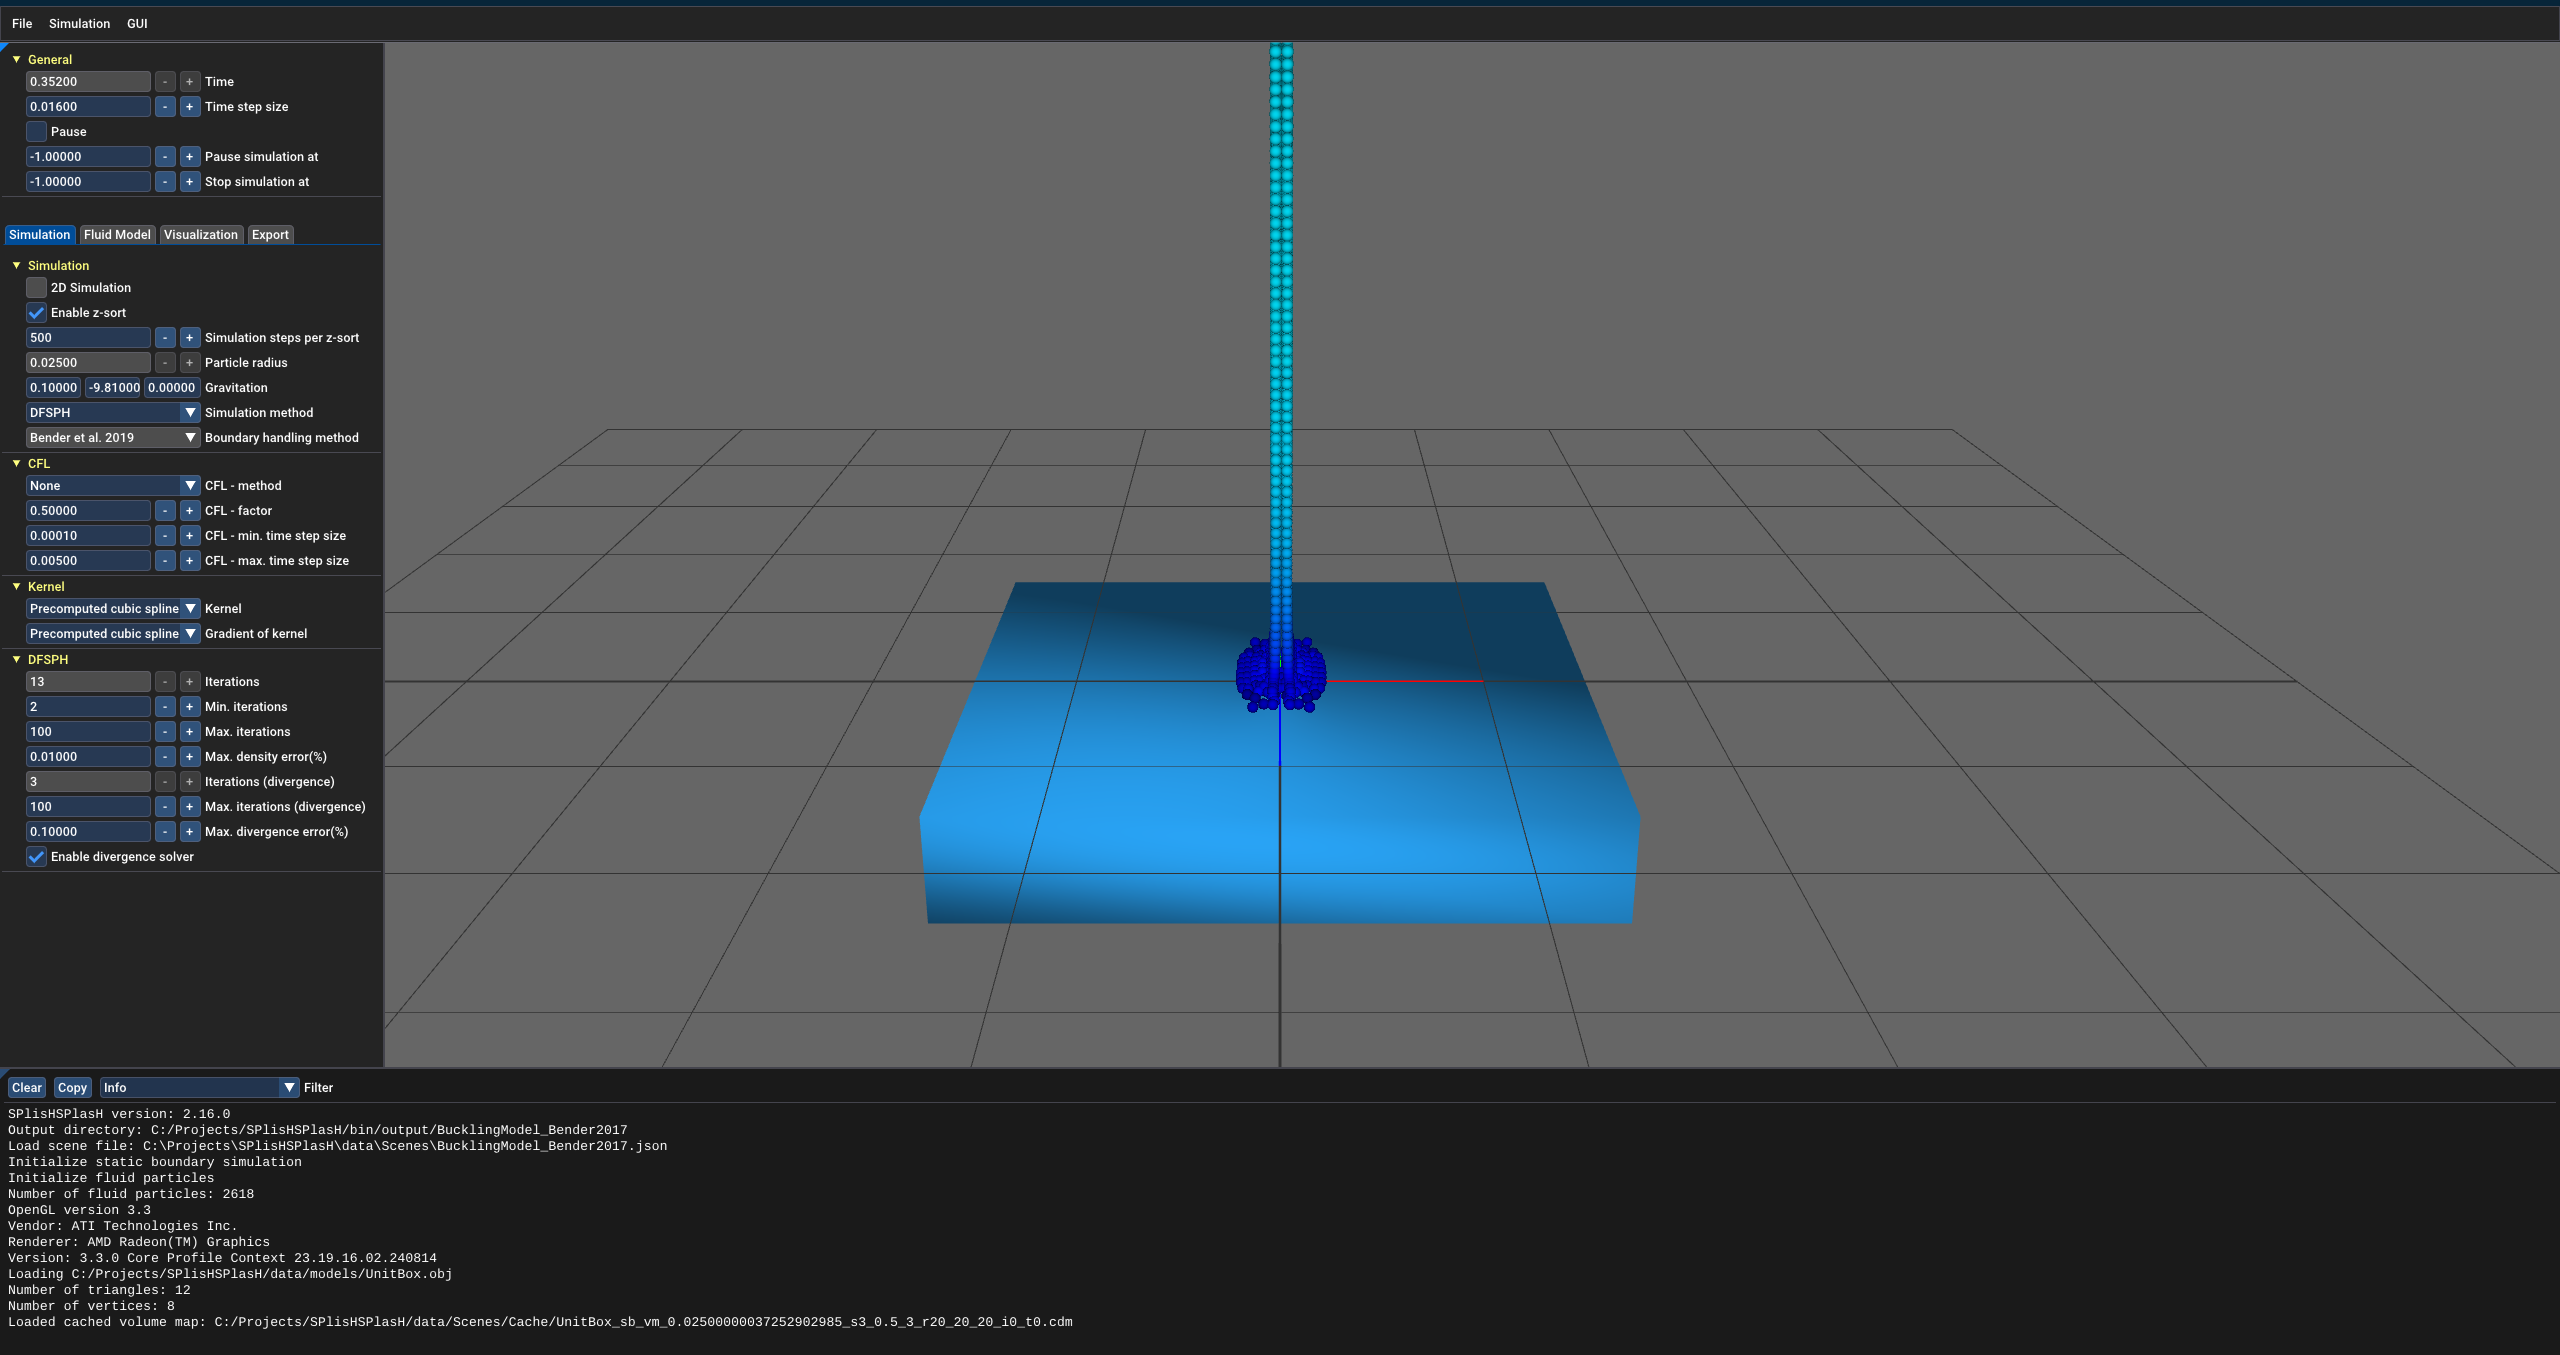
\includegraphics[width=0.85\textwidth]{figures/splishsplash.png}
    \caption{Symulacja cieczy w bibliotece SPlisHSPlasH z aktywnym solverem DFSPH i panelem konfiguracji parametrów fizycznych \newline Źródło: Własne opracowanie na podstawie dokumentacji biblioteki \cite{SPlisHSPlasH_Library}}

    \label{fig:splishsplash}
\end{figure}

\subsection{Podsumowanie rozwiązań i kontekst projektu}

Podsumowując przegląd istniejących rozwiązań, można wskazać na istotne różnice w ich architekturze oraz zastosowaniach. 
Blender jest środowiskiem nastawionym na generowanie wysokiej jakości animacji, które wymagają wcześniejszego przeliczenia.
Unreal Engine 5 z systemem Niagara oferuje wysoką wydajność w środowisku interaktywnym, lecz opiera 
się na złożonej, wysokopoziomowej architekturze silnika gry. SPlisHSPlasH z kolei jest biblioteką koncentrującą 
się na obliczeniach równoległych na procesorze w celach naukowych.

Niniejsza praca stanowi implementację algorytmu DFSPH z wykorzystaniem nowoczesnego stosu technologicznego: 
języka Rust oraz API Vulkan. W odróżnieniu od omawianych systemów, projekt skupia się na pełnym przeniesieniu 
potoku obliczeniowego na procesor graficzny przy zachowaniu niskopoziomowej kontroli nad zasobami sprzętowymi. 
Bezpośrednie porównanie cech technicznych opisanych rozwiązań z systemem opracowanym w ramach pracy przedstawiono 
w tabeli~\ref{tab:solutions_comparison}. Wybór tego podejścia wynika z chęci zbadania granic wydajności i jakości, 
jakie można osiągnąć dzięki nowoczesnym technologiom programistycznym, oraz z potrzeby stworzenia elastycznej 
platformy do dalszych eksperymentów z algorytmami SPH.

\begin{table}[ht]
    \centering
    \caption{Porównanie istniejących rozwiązań symulacji cieczy z niniejszą pracą}
    \label{tab:solutions_comparison}
    \small
    \begin{tabular}{lcccc}
    \toprule
    Cecha & Blender & Unreal Engine 5 & SPlisHSPlasH & Niniejsza praca \\ \midrule
    Metoda symulacji       & FLIP      & FLIP          & SPH       & SPH (DFSPH) \\
    Czas rzeczywisty       & Nie       & Tak           & Nie       & Tak         \\
    Obliczenia GPU         & Częściowe & Tak           & Częściowe & Tak (w pełni) \\
    Otwarte źródło         & Tak       & Tak           & Tak       & Tak         \\
    Język implementacji    & C++       & C++           & C++       & Rust        \\
    API graficzne          & OpenGL    & DX12 / Vulkan & OpenGL    & Vulkan      \\
    \bottomrule
    \end{tabular}
\end{table}

% ----------------------------------------------------------------

\section{Język programowania Rust}

Rust jest wieloparadygmatowym językiem programowania systemowego, zaprojektowanym przez pracowników Mozilla Research i opublikowanym w pierwszej stabilnej wersji w 2015 roku \cite{rust-book}. Od 2021 roku jego rozwój nadzoruje niezależna fundacja Rust Foundation. Język został stworzony z myślą o wypełnieniu niszy zajmowanej dotychczas przez C i C++ --- oferuje porównywalną wydajność obliczeniową przy jednoczesnym wyeliminowaniu całej klasy błędów wynikających z ręcznego zarządzania pamięcią.

Centralną innowacją języka jest system własności, który pozwala kompilatorowi weryfikować poprawność zarządzania pamięcią statycznie --- bez konieczności stosowania odśmiecacza pamięci. W odróżnieniu od języków zarządzanych, takich jak Java czy C\#, programy w Rust nie ponoszą kosztów przerw wywołanych odśmiecaniem. Jednocześnie, w odróżnieniu od C i C++, kompilator gwarantuje brak niezdefiniowanych zachowań w bezpiecznym kodzie: wiszące wskaźniki, przepełnienia buforów i wyścigi danych są weryfikowane statycznie i odrzucane już na etapie kompilacji. Brak wskaźników null jest egzekwowany przez typ \texttt{Option<T>}, natomiast obsługa błędów opiera się na typie \texttt{Result<T,\,E>}, wymuszającym jawne rozpatrzenie każdego przypadku wyjątkowego. Rust nie zapewnia jednak automatycznej ochrony w blokach oznaczonych jako \texttt{unsafe} --- programista przejmuje wówczas pełną odpowiedzialność za poprawność operacji niskopoziomowych, co jest niezbędne przy bezpośredniej komunikacji z API graficznym.

W odróżnieniu od języków obiektowych Rust nie posiada klas --- dane
i zachowanie są rozdzielone: struktury (ang.~\textit{structs}) przechowują
pola, a bloki \textit{impl} definiują operujące na nich metody.
Rolę interfejsów pełnią cechy (ang.~\textit{traits}) --- określają
kontrakt metod, który dowolny typ może spełnić niezależnie od swojej
wewnętrznej reprezentacji.

Ekosystem języka Rust opiera się na wbudowanym menedżerze pakietów 
Cargo oraz publicznym repozytorium crates.io. Podstawową jednostką dystrybucji
kodu jest skrzynka (ang.~\textit{crate}) --- pakiet kodu Rust przyjmujący 
formę biblioteki lub programu wykonywalnego. Repozytorium crates.io pełni rolę analogiczną 
do PyPI w Pythonie czy npm w JavaScript, pozwalając na deklaratywne zarządzanie zależnościami 
bezpośrednio w pliku konfiguracyjnym projektu, bez potrzeby instalowania zewnętrznych narzędzi. 
W niniejszym projekcie zastosowano szereg bibliotek uzupełniających. Zarządzanie oknem aplikacji 
i obsługę pętli zdarzeń zapewnia \texttt{winit} \cite{winit}. Obliczenia algebraiczne po stronie CPU, 
wektory i macierze przekształceń, realizuje \texttt{glam} \cite{glam}, biblioteka zoptymalizowana pod kątem 
instrukcji SIMD. Interfejs użytkownika do konfiguracji parametrów symulacji w czasie rzeczywistym 
zbudowano przy użyciu \texttt{egui} \cite{egui} z integracją \texttt{egui\_winit\_vulkano} \cite{egui-winit-vulkano}. 
Obsługę błędów na poziomie modułów i aplikacji upraszczają odpowiednio \texttt{thiserror} \cite{thiserror} i \texttt{anyhow} \cite{anyhow}, 
natomiast ujednoliconą infrastrukturę logowania dostarcza para \texttt{log} \cite{log-rs} i \texttt{simple\_logger} \cite{simple-logger}.

\begin{table}[ht]
    \centering
    \caption{Porównanie języków Rust i C++ pod względem cech istotnych dla programowania systemowego}
    \label{tab:rust_vs_cpp}
    \small
    \begin{tabular}{lcc}
    \toprule
    Cecha & C++ & Rust \\ \midrule
    Bezpieczeństwo pamięci      & Manualne              & Gwarantowane przez kompilator \\
    Odśmiecacz pamięci          & Nie                   & Nie                           \\
    Niezdefiniowane zachowania  & Możliwe               & Niemożliwe (safe Rust)        \\
    Wyścigi danych              & Możliwe               & Niemożliwe (czas kompilacji)  \\
    Wskaźniki null              & Tak                   & Nie (\texttt{Option<T>})      \\
    Zerowe koszty abstrakcji    & Tak                   & Tak                           \\
    Standardowy menedżer pakietów & Brak                & Cargo                         \\
    Dojrzałość ekosystemu       & Wysoka (od 1983)      & Rosnąca (od 2015)             \\
    \bottomrule
    \end{tabular}
\end{table}

Rust jest coraz powszechniej postrzegany jako naturalny następca C++ w nowych projektach systemowych. Organizacje takie jak Microsoft, Google i Linux Foundation włączyły go już do swoich stosów technologicznych jako odpowiedź na rosnące wymagania w zakresie bezpieczeństwa oprogramowania. Jako język oferujący zerowe koszty abstrakcji, rozbudowany system typów i statyczne gwarancje poprawności bez narzutu czasowego, Rust eliminuje całą klasę błędów trudnych do debugowania w złożonych systemach wielowątkowych - co czyni go szczególnie trafnym wyborem dla implementacji silnika symulacji cieczy opisanego w niniejszej pracy.

% ----------------------------------------------------------------

\section{API graficzne Vulkan}

Vulkan jest niskopoziomowym, wieloplatformowym interfejsem programowania graficznego, 
opracowanym przez konsorcjum Khronos Group i opublikowanym w 2016 roku \cite{vulkan-spec}. 
Jego geneza wynika z narastających ograniczeń architektury OpenGL, 
która przez ponad dwie dekady rozrastało się o kolejne warstwy abstrakcji i 
niejawne mechanizmy zarządzania zasobami. Sterownik OpenGL pełnił rolę rozbudowanego 
pośrednika: sam synchronizował polecenia GPU, podejmował decyzje o alokacji pamięci i 
kompilował shadery w nieokreślonych momentach, co prowadziło do znacznego narzutu procesora głównego, 
uniemożliwiało efektywną wielowątkowość i skutkowało nieprzewidywalnym zachowaniem w sytuacjach granicznych. 
Bezpośrednim poprzednikiem Vulkana jest biblioteka Mantle \cite{amdmantle2015}, opracowana przez AMD we współpracy z~deweloperami 
gier w 2013 roku, stanowiąca pierwszą propozycję niskopoziomowego API graficznego, która wykazała, 
że jawne przejęcie przez programistę kontroli nad sprzętem przekłada się na mierzalne zyski wydajnościowe.

Centralną filozofią Vulkana jest jawność i determinizm. Każdy zasób, taki jak bufor pamięci, 
obraz, potok obliczeniowy, jest tworzony i zarządzany przez programistę w sposób jawny, 
a każda operacja synchronizacji między procesorem a GPU musi być ręcznie zdefiniowana. 
Rezygnacja z globalnego automatu stanów na rzecz izolowanych, niezależnych obiektów umożliwia 
równoległe budowanie potoków poleceń w wielu wątkach bez ryzyka konfliktu stanu. 
Ujednoliconym wzorcem inicjalizacji w API Vulkan jest wykorzystanie struktur opisowych. 
Tworzenie dowolnego obiektu wymaga od programisty wypełnienia~dedykowanej struktury konfiguracyjnej, 
która precyzyjnie definiuje jego parametry, a następnie przekazania jej do odpowiedniej funkcji tworzącej. 
Podejście to, stosowane konsekwentnie w całym standardzie, sprawia, że konfiguracja systemu jest w pełni jawna. 
Pozwala to na precyzyjne określenie zależności między obiektami już na poziomie kodu, co eliminuje domyślne stany 
sterownika graficznego.

Drugą fundamentalną cechą Vulkana jest system rozszerzeń, zaprojektowany jako integralna 
część architektury API od pierwszej wersji specyfikacji. Rdzeń Vulkana jest celowo minimalny i stabilny: 
obejmuje wyłącznie operacje wspólne dla wszystkich implementacji sprzętowych. 
Wszelkie funkcjonalności specyficzne dla producenta lub nowsze możliwości renderowania 
udostępniane są przez rozszerzenia aktywowane jawnie przy tworzeniu instancji lub urządzenia. 
Rozszerzenia dzielą się na trzy kategorie: rozszerzenia producenta sprzętu (np.\ \texttt{VK\_NV\_*} lub
\texttt{VK\_AMD\_*}), rozszerzenia wieloproducentowe (\texttt{VK\_EXT\_*}) oraz rozszerzenia
ratyfikowane przez Khronos (\texttt{VK\_KHR\_*}).

Ostatnia kategoria powstaje w~drodze konsensusu wszystkich członków organizacji Khronos~---
AMD, NVIDIA, Intel, ARM, Google, Apple i~innych --- i~pełni dwojaką rolę.
Po pierwsze, dostarcza krytyczne funkcjonalności obsługiwane przez wszystkie współczesne karty graficzne,
które z~różnych powodów nie trafiły do rdzenia specyfikacji; przykładem jest \texttt{VK\_KHR\_swapchain}
umożliwiający prezentację obrazu na ekranie systemu operacyjnego, czy \texttt{VK\_KHR\_ray\_tracing\_pipeline}
wprowadzający sprzętowe śledzenie promieni.
Po drugie, rozszerzenia \texttt{KHR} pełnią rolę oficjalnej ,,\textit{poczekalni}'' dla nowych technologii:
zamiast pospiesznie modyfikować stabilny rdzeń, Khronos publikuje rozszerzenie, pozwala deweloperom
je przetestować w~warunkach produkcyjnych, a~jeśli okaże się ono dojrzałe~--- włącza je do kolejnej
wersji specyfikacji rdzeniowej (ang.~\textit{core specification}). Mechanizm ten był stosowany konsekwentnie 
w~wersjach Vulkan 1.1, 1.2 i~1.3, do których przeniesiono łącznie kilkadziesiąt wcześniejszych rozszerzeń \texttt{KHR}.

Podejście to umożliwia producentom sprzętu udostępnianie możliwości swoich układów
bez naruszania globalnej kompatybilności, pozwalając jednocześnie programiście na jawne deklarowanie
funkcjonalności wymaganych przez aplikację.

\subsection{Instancja, urządzenie fizyczne i logiczne}
\label{sec:vulkan_hierarchy}

\texttt{VkInstance} jest punktem wejścia do środowiska uruchomieniowego Vulkana i
korzeniem całej hierarchii obiektów API. Jej utworzenie ładuje sterownik Vulkana
i inicjalizuje rozszerzenia działające na poziomie instancji, które dotyczą
platformy systemowej, a nie konkretnego układu graficznego. Przykładem jest
\texttt{VK\_KHR\_surface}, które definiuje abstrakcję powierzchni okienkowej niezależną
od systemu operacyjnego, oraz towarzyszące mu rozszerzenia platformowe, takie jak
\texttt{VK\_KHR\_win32\_surface} czy \texttt{VK\_KHR\_xcb\_surface}, odpowiadające
za integrację z konkretnym podsystemem okienkowym. Rozszerzenia instancji
aktywuje się przy jej tworzeniu, deklarując ich nazwy w strukturze \texttt{VkInstanceCreateInfo}.

Po utworzeniu instancji możliwe jest wyliczenie dostępnych urządzeń fizycznych.
\texttt{VkPhysicalDevice} reprezentuje jeden fizyczny układ graficzny widoczny dla systemu.
Na stacji roboczej może znajdować się kilka takich układów, w tym zintegrowany procesor 
graficzny wbudowany w jednostkę centralną oraz dedykowana karta graficzna. Vulkan pozwala
programiście odpytać każde z nich o właściwości: typ urządzenia (dyskretna karta graficzna,
układ zintegrowany, CPU), limity sprzętowe, obsługiwane formaty obrazów i funkcjonalności.
Na tej podstawie aplikacja może samodzielnie wybrać najbardziej odpowiedni układ lub
umożliwić taki wybór użytkownikowi.

Wykorzystując wybrany układ fizyczny, programista tworzy urządzenie logiczne
\texttt{VkDevice}, stanowiące centralny obiekt API, z którym powiązane są wszystkie kolejki poleceń, 
bufory, obrazy oraz potoki obliczeniowe. Na tym etapie aktywowane są
rozszerzenia działające na poziomie urządzenia, czyli dotyczące możliwości konkretnego
układu graficznego. Rozróżnienie poziomów ma praktyczne znaczenie: \texttt{VK\_KHR\_surface}
jest rozszerzeniem instancji, bo integracja z oknem systemu operacyjnego jest kwestią
platformową; \texttt{VK\_KHR\_swapchain}, czyli mechanizm prezentowania klatek na ekranie,
jest już rozszerzeniem urządzenia, bo wymaga fizycznego wyjścia wyświetlacza. Układ
graficzny w serwerze bez monitora może nie obsługiwać \texttt{VK\_KHR\_swapchain} w ogóle,
lecz nadal będzie w pełni zdolny do obliczeń ogólnego przeznaczenia na GPU. Taki podział
pozwala aplikacji jawnie deklarować wymagane zależności sprzętowe zamiast zakładać
obecność możliwości, których dany układ może nie posiadać.
Relację między trzema warstwami inicjalizacyjnymi ilustruje rysunek~\ref{fig:vulkan_hierarchy}.

\begin{figure}[ht]
\centering
\begin{tikzpicture}[
  vkbox/.style={rectangle, draw=black!80, fill=white, rounded corners=3pt,
    minimum width=4.4cm, minimum height=0.72cm, align=center, font=\small\ttfamily},
  vkfade/.style={rectangle, draw=black!25, fill=gray!6, text=black!30, rounded corners=3pt,
    minimum width=4.4cm, minimum height=0.72cm, align=center, font=\small\ttfamily},
  resbox/.style={rectangle, draw=black!80, fill=white, rounded corners=3pt,
    minimum width=3.2cm, minimum height=0.72cm, align=center, font=\small\ttfamily},
  arr/.style={->, >=Stealth, semithick},
  faint/.style={->, >=Stealth, semithick, draw=black!25}
]
  \node[vkbox]  (inst)  at (0,      0)   {VkInstance};
  \node[vkbox]  (phys0) at (-3.2,  -2.0) {VkPhysicalDevice [0]};
  \node[vkfade] (phys1) at ( 3.2,  -2.0) {VkPhysicalDevice [1]};
  \node[vkbox]  (dev)   at (0,     -4.0) {VkDevice};
  \node[resbox] (queue) at (-3.6,  -5.9) {VkQueue};
  \node[resbox] (res)   at (0,     -5.9) {VkBuffer,~VkImage};
  \node[resbox] (pipe)  at ( 3.6,  -5.9) {VkPipeline};

  \draw[arr]   (inst)  -- (phys0);
  \draw[faint] (inst)  -- (phys1);
  \draw[arr]   (phys0) -- (dev);
  \draw[arr]   (dev)   -- (queue);
  \draw[arr]   (dev)   -- (res);
  \draw[arr]   (dev)   -- (pipe);
\end{tikzpicture}
\caption{Hierarchia inicjalizacyjna Vulkana. Instancja daje dostęp do urządzeń fizycznych,
z których jedno wybierane jest do utworzenia urządzenia logicznego \texttt{VkDevice}, będącego
punktem zaczepu wszystkich pozostałych obiektów API. Szary węzeł oznacza niewybrany układ fizyczny
\newline Źródło: Opracowanie własne na podstawie specyfikacji \cite{vulkan-spec}}
\label{fig:vulkan_hierarchy}
\end{figure}

\subsection{Kolejki i pule poleceń}

Nowoczesne karty graficzne udostępniają wiele sprzętowych kolejek poleceń, przez które
procesor przekazuje pracę do wykonania na GPU. Vulkan grupuje je w rodziny kolejek, 
z których każda obsługuje określony zestaw operacji. Typowa karta graficzna eksponuje co 
najmniej rodzinę graficzną, obsługującą rysowanie i prezentację klatek, oraz rodzinę obliczeniową, 
przeznaczoną do obliczeń ogólnego przeznaczenia. Wiele układów udostępnia też 
wyspecjalizowaną rodzinę transferową, zoptymalizowaną sprzętowo do kopiowania danych
między pamięcią systemową procesora głównego a~dedykowaną pamięcią karty graficznej.
W nomenklaturze Vulkana strona procesorowa systemu, obejmująca procesor główny i pamięć RAM,
określana jest terminem \textit{host}, zaś strona układu graficznego wraz z jego pamięcią
wideo terminem \textit{device}.
Programista odpytuje wybrany \texttt{VkPhysicalDevice} o dostępne rodziny i deklaruje,
z których z nich chce korzystać, w strukturze \texttt{VkDeviceCreateInfo} przekazywanej
przy tworzeniu urządzenia logicznego. Efektem jest zbiór uchwytów \texttt{VkQueue},
z których każdy reprezentuje jedną kolejkę danej rodziny.

Samo polecenie nie jest przekazywane do kolejki bezpośrednio jako wywołanie funkcji.
Zamiast tego Vulkan stosuje model rejestrowania odroczonych poleceń. Programista tworzy
\texttt{VkCommandPool}, obiekt zarządzający pamięcią przeznaczoną na polecenia, powiązany
z konkretną rodziną kolejek. Z puli tej alokowane są bufory poleceń \texttt{VkCommandBuffer},
w których rejestruje się sekwencje operacji GPU. Operacje te obejmują przesłania danych
między buforami, bariery synchronizacji, uruchomienia potoków graficznych oraz wywołania
obliczeniowe, określane terminem \textit{dispatch}. Bufor poleceń rejestruje całą sekwencję
operacji po stronie procesora głównego, a następnie przekazywany jest do kolejki jednym
wywołaniem funkcji wysyłającej. GPU przetwarza zarejestrowane polecenia asynchronicznie
względem procesora, co jest zasadniczą różnicą w stosunku do modelu OpenGL, gdzie każde
wywołanie API było natychmiastowym żądaniem wykonywanym przez sterownik.

Rozdzielenie rejestrowania od wysyłania przynosi dwie praktyczne konsekwencje. Po pierwsze,
wiele wątków procesora może jednocześnie rejestrować polecenia w niezależnych buforach,
korzystając z osobnych pul powiązanych z tą samą rodziną kolejek. Po drugie, bufor poleceń
reprezentujący stały zestaw pracy, który nie zmienia się między klatkami, może być
zarejestrowany raz i wysyłany wielokrotnie bez ponownego budowania.

\subsection{Łańcuch wymiany i dynamiczne renderowanie}
\label{sec:vulkan_swapchain}

Renderowanie w czasie rzeczywistym polega na cyklicznym generowaniu kolejnych obrazów klatki
i przesyłaniu ich na ekran. Konieczność synchronizacji tego procesu z monitorem wynika
z fundamentalnej właściwości sprzętu wyświetlającego: monitor odświeża obraz ze stałą
częstotliwością, odczytując zawartość bufora wideo z pamięci karty graficznej.
Jeśli aplikacja zapisuje nową klatkę bezpośrednio do obszaru, który monitor właśnie odczytuje,
na ekranie pojawia się artefakt rozrywania obrazu (ang.~\textit{screen tearing}):
górna część klatki pochodzi z poprzedniego obrazu, a dolna z~aktualnie zapisywanego.
Rozwiązaniem jest oddzielenie bufora wyświetlanego od bufora roboczego i podmiana ich zawartości
dopiero po zakończeniu cyklu odświeżania. W odróżnieniu od OpenGL, które ukrywało ten
mechanizm za pojęciem domyślnego bufora ramki, Vulkan wymaga jawnego skonstruowania tej
infrastruktury w postaci łańcucha wymiany (ang.~\textit{swapchain}).

Łańcuch wymiany jest zestawem obrazów zarządzanych przez system okienkowy, przeznaczonych
do prezentacji na ekranie. Aplikacja pobiera jeden z dostępnych obrazów, rysuje do niego
klatkę, a następnie oddaje go do kolejki prezentacji, skąd trafia on na ekran w odpowiednim
momencie. Liczba obrazów w łańcuchu jest konfigurowalna: przy dwóch obrazach jeden jest
wyświetlany, a drugi przygotowywany, co określa się mianem podwójnego buforowania
(ang.~\textit{double buffering}); przy trzech obrazach aplikacja może przygotowywać kolejną klatkę
jeszcze zanim poprzednio złożona dotrze na ekran, co nosi nazwę potrójnego buforowania
(ang.~\textit{triple buffering}) i zmniejsza ryzyko przestojów renderowania kosztem nieznacznie
wyższego opóźnienia. Sposób synchronizacji z częstotliwością odświeżania monitora określa
tryb prezentacji: tryb \texttt{FIFO} odpowiada klasycznej synchronizacji pionowej, a tryb
\texttt{MAILBOX} zastępuje oczekujący obraz nowszym, jeśli ten jest już gotowy, minimalizując
widoczne opóźnienie klatki.

Vulkan oferuje dwa podejścia do przekazania poleceń rysowania do obrazu łańcucha wymiany:
model tradycyjny oparty na jawnie skompilowanych obiektach przejścia renderowania i bufora ramki
oraz dynamiczne renderowanie, wprowadzone jako funkcja rdzeniowa w wersji 1.3.
W modelu tradycyjnym przejście renderowania (\texttt{VkRenderPass}) jest deklaratywnym opisem struktury operacji
rysowania: definiuje, jakie załączniki obrazowe będą używane, w jakim formacie, co ma się
stać z ich zawartością na początku przejścia (wyczyszczenie lub zachowanie) i na końcu
(zachowanie lub odrzucenie). Opis ten jest kompilowany przez sterownik z wyprzedzeniem,
co pozwala mu na optymalizację dostępów do pamięci. Bufor ramki (\texttt{VkFramebuffer})
wiąże konkretne widoki obrazów (\texttt{VkImageView}) z załącznikami zadeklarowanymi
w przejściu renderowania. Ponieważ łańcuch wymiany dostarcza zestaw obrazów, a nie jeden,
aplikacja tworzy osobny bufor ramki dla każdego obrazu w łańcuchu i wybiera właściwy
przy budowaniu bufora poleceń danej klatki.
Oba podejścia, tradycyjne i dynamiczne, zestawia rysunek~\ref{fig:vulkan_rendering_path}.

\begin{figure}[ht]
\centering
\begin{tikzpicture}[
  fbox/.style={rectangle, draw=black!80, fill=white, rounded corners=3pt,
    minimum width=4.6cm, minimum height=0.72cm, align=center, font=\small\ttfamily},
  hbox/.style={rectangle, draw=black!80, fill=gray!14, rounded corners=3pt,
    minimum width=4.6cm, minimum height=0.72cm, align=center, font=\small\ttfamily},
  mbox/.style={rectangle, draw=black!60, fill=black!6, rounded corners=3pt,
    minimum width=4.6cm, minimum height=0.72cm, align=center, font=\small\sffamily},
  arr/.style={->, >=Stealth, semithick},
  tit/.style={font=\small\bfseries\sffamily, align=center}
]
  \node[tit] at (-3.0,  0.5) {Tradycyjny model};
  \node[tit] at ( 3.0,  0.5) {Dynamiczne renderowanie};
  \draw[black!18, dashed, thin] (0, 0.85) -- (0, -6.1);

  % --- Left column ---
  \node[fbox] (ls) at (-3.0, -0.40) {VkImage (swapchain)};
  \node[fbox] (lv) at (-3.0, -1.35) {VkImageView};
  \node[hbox] (lr) at (-3.0, -2.30) {VkRenderPass};
  \node[hbox] (lf) at (-3.0, -3.25) {VkFramebuffer};
  \node[fbox] (lc) at (-3.0, -4.20) {Komendy rysowania};
  \node[mbox] (lm) at (-3.0, -5.30) {Monitor};

  \draw[arr] (ls) -- (lv);
  \draw[arr] (lv) -- (lr);
  \draw[arr] (lr) -- (lf);
  \draw[arr] (lf) -- (lc);
  \draw[arr] (lc) -- (lm);

  % --- Right column ---
  \node[fbox] (rs) at (3.0, -0.40)  {VkImage (swapchain)};
  \node[fbox] (rv) at (3.0, -1.35)  {VkImageView};
  \node[fbox] (rd) at (3.0, -2.775) {vkCmdBeginRendering};
  \node[fbox] (rc) at (3.0, -4.20)  {Komendy rysowania};
  \node[mbox] (rm) at (3.0, -5.30)  {Monitor};

  \draw[arr] (rs) -- (rv);
  \draw[arr] (rv) -- (rd);
  \draw[arr] (rd) -- (rc);
  \draw[arr] (rc) -- (rm);
\end{tikzpicture}
\caption{Porównanie ścieżek renderowania w Vulkanie. Zacienione pola w modelu tradycyjnym
(\texttt{VkRenderPass} i \texttt{VkFramebuffer}) są zbędne w dynamicznym renderowaniu,
które deklaruje załączniki bezpośrednio w buforze poleceń
\newline Źródło: Opracowanie własne na podstawie specyfikacji \cite{vulkan-spec}}
\label{fig:vulkan_rendering_path}
\end{figure}

W modelu dynamicznego renderowania programista deklaruje używane załączniki bezpośrednio
w buforze poleceń, tuż przed poleceniami rysowania, zamiast opisywać je z wyprzedzeniem
w dedykowanym obiekcie kompilowanym przez sterownik. Eliminuje to potrzebę utrzymywania
zgodności między przejściami renderowania a potokami graficznymi i lepiej odpowiada
architekturom, w których zestaw załączników zmienia się między krokami renderowania.

\subsection{Zasoby: bufory, obrazy i deskryptory}

Pojęcie \texttt{VkImage} pojawiło się już przy omawianiu łańcucha wymiany jako kontener
klatki gotowej do prezentacji. W szerszym sensie obraz jest zasobem GPU reprezentującym
wielowymiarową tablicę danych pikselowych, opisaną formatem (np.\ \texttt{VK\_FORMAT\_R32\_SFLOAT}),
rozmiarem i liczbą poziomów mipmap (prekalkulowanych kopii obrazu w malejących rozdzielczościach). 
Sprzęt przechowuje obrazy w wewnętrznym układzie
kafelkowym, zoptymalizowanym pod kątem lokalności dostępów podczas próbkowania i zapisu.
Programista nie adresuje obrazu bezpośrednio: każdy dostęp odbywa się przez
\texttt{VkImageView}, który deklaruje format interpretacji i zakres odczytywanego podzasobu.

Bufor (\texttt{VkBuffer}) jest ciągłym obszarem pamięci GPU bez narzuconej struktury
wewnętrznej. Jego semantykę określają flagi użycia przekazane przy tworzeniu oraz sposób,
w jaki shadery go odczytują i zapisują. Tworzenie bufora składa się z dwóch etapów:
najpierw tworzy się obiekt \texttt{VkBuffer} opisujący rozmiar i zamierzone użycie,
a następnie przydziela się mu pamięć wybraną z odpowiedniego stosu. Vulkan eksponuje
wiele stosów pamięci o różnych własnościach: pamięć lokalna dla urządzenia
(ang.~\textit{device-local}) rezyduje wyłącznie po stronie układu graficznego
i oferuje najwyższą przepustowość, natomiast pamięć widoczna dla procesora
(ang.~\textit{host-visible}) jest dostępna do bezpośredniego zapisu przez procesor główny.
W praktyce zarządzanie tym procesem deleguje się do biblioteki Vulkan Memory Allocator~(VMA) \cite{vma-library},
opracowanej przez AMD: programista deklaruje wyłącznie przeznaczenie bufora,
a VMA dobiera właściwy stos pamięci i zarządza jego fragmentacją.
Aby załadować dane przygotowane po stronie procesora do bufora rezydującego w pamięci
lokalnej dla urządzenia, stosuje się bufor pośredniczący (ang.~\textit{staging buffer}):
tymczasowy bufor w pamięci widocznej dla procesora, wypełniany przez CPU, którego
zawartość kopiowana jest następnie przez rodzinę kolejek transferowych do docelowej
pamięci układu graficznego.

Flagi użycia determinują dozwolone operacje na buforze i wpływają na wybór stosu pamięci
przez VMA. Tabela~\ref{tab:buffer_types} zestawia typy buforów istotne dla niniejszej
implementacji.

\begin{table}[ht]
\centering
\caption{Typy buforów Vulkana i ich zastosowanie}
\label{tab:buffer_types}
\small
\begin{tabular}{lp{9.5cm}}
\toprule
Typ bufora & Zastosowanie \\
\midrule
Wierzchołkowy & Dane wierzchołków przekazywane bezpośrednio do potoku graficznego \\ 
\addlinespace
Jednorodny (UBO) & Małe, stałe dane odczytywane w shaderach: macierze transformacji, parametry symulacji \\
\addlinespace
Składowania (SSBO) & Duże dane dostępne do odczytu i zapisu w shaderach obliczeniowych; główny nośnik stanu symulacji \\
\addlinespace
Pośredniczący (Staging) & Tymczasowy bufor w pamięci host-visible służący do transferu danych inicjalizacyjnych z CPU do pamięci device-local \\
\bottomrule
\end{tabular}
\end{table}

Shadery nie adresują buforów i obrazów bezpośrednio przez wskaźnik; zasoby te wiązane są
z potokiem obliczeniowym za pośrednictwem zestawów deskryptorów.
Schemat powiązań deklarowany jest w obiekcie \texttt{VkDescriptorSetLayout}, który precyzuje,
jakiego rodzaju zasoby oczekiwane są na każdym miejscu wiązania shaderów.
Alokacją zestawów zarządza \texttt{VkDescriptorPool}: obiekt rezerwujący z góry blok pamięci
przeznaczony wyłącznie na zestawy danego układu, analogicznie do roli,
jaką \texttt{VkCommandPool} pełni wobec buforów poleceń.
Z puli alokowany jest \texttt{VkDescriptorSet}, wiążący konkretne uchwyty
\texttt{VkBuffer} i \texttt{VkImageView} ze zdefiniowanymi miejscami wiązania.
Układ potoków \texttt{VkPipelineLayout} agreguje jeden lub kilka takich układów zestawów
i jest wbudowywany w każdy potok obliczeniowy przy jego tworzeniu, dzięki czemu sterownik
zna pełen schemat zasobów wymaganych przez shadery już na etapie kompilacji.
Zależności między wymienionymi obiektami ilustruje rysunek~\ref{fig:vulkan_resources}.

\begin{figure}[ht]
\centering
\begin{tikzpicture}[
  vkbox/.style={rectangle, draw=black!80, fill=white, rounded corners=3pt,
    minimum width=4.0cm, minimum height=0.72cm, align=center, font=\small\ttfamily},
  mbox/.style={rectangle, draw=black!60, fill=black!7, rounded corners=3pt,
    minimum width=4.6cm, minimum height=0.72cm, align=center, font=\small\sffamily},
  arr/.style={->, >=Stealth, semithick},
  refarr/.style={->, >=Stealth, semithick, dashed, draw=black!55}
]
  \node[mbox]  (vma)     at (0,     0)    {Vulkan Memory Allocator};
  \node[vkbox] (buf)     at (-2.8, -1.8)  {VkBuffer};
  \node[vkbox] (img)     at ( 2.8, -1.8)  {VkImage};
  \node[vkbox] (view)    at ( 2.8, -3.2)  {VkImageView};

  \draw[arr] (vma)  -- (buf);
  \draw[arr] (vma)  -- (img);
  \draw[arr] (img)  -- (view);

  \draw[black!18, dashed, thin] (-5.5, -4.3) -- (5.5, -4.3);

  \node[vkbox] (pool)    at (-3.2, -5.5)  {VkDescriptorPool};
  \node[vkbox] (dlayout) at ( 3.2, -5.5)  {VkDescriptorSetLayout};
  \node[vkbox] (dset)    at (0,    -7.0)  {VkDescriptorSet};
  \node[vkbox] (playout) at (0,    -8.6)  {VkPipelineLayout};

  \draw[arr] (pool)    -- (dset);
  \draw[arr] (dlayout) -- (dset);
  \draw[arr] (dset)    -- (playout);

  \draw[refarr] (buf)  to[bend right=15] (dset);
  \draw[refarr] (view) to[bend left=15]  (dset);
\end{tikzpicture}
\caption{Schemat zarządzania zasobami i powiązań deskryptorowych w Vulkanie.
Górna warstwa przedstawia alokację zasobów przez VMA; dolna warstwa pokazuje
mechanizm deskryptorów. Przerywane strzałki oznaczają referencje
\texttt{VkDescriptorSet} do konkretnych buforów i widoków obrazów
\newline Źródło: Opracowanie własne na podstawie specyfikacji \cite{vulkan-spec}}
\label{fig:vulkan_resources}
\end{figure}

\subsection{Potok obliczeniowy i graficzny}
\label{subsec:pipeline}

Potok graficzny lub obliczeniowy jest skompilowanym, niezmiennym obiektem zawierającym
kompletną konfigurację przetwarzania GPU. Vulkan nie przyjmuje shaderów w postaci kodu
źródłowego, lecz w formacie SPIR-V (ang.~\textit{Standard Portable Intermediate
Representation}): przenośnego bytekodu zdefiniowanego przez Khronos Group, który zastępuje
tekstowe źródła GLSL przyjmowane przez OpenGL. Kompilacja shaderów do SPIR-V odbywa się
statycznie przed uruchomieniem aplikacji, co umożliwia wczesne wykrycie błędów składniowych
i eliminuje niedeterministyczne opóźnienia kompilacji w trakcie działania programu.
Sterownik kompiluje ten bytekod do natywnych instrukcji konkretnej karty graficznej przy
tworzeniu potoku i scala je z parametrami etapów stałofunkcyjnych. Ponieważ ta operacja
jest kosztowna, potoki tworzy się jednorazowo podczas inicjalizacji i wiąże w buforach
poleceń bez ponownej kompilacji. Vulkan rozróżnia dwa typy potoków: potok graficzny,
służący do~rasteryzowanego przetwarzania geometrii, oraz potok obliczeniowy, przeznaczony
do równoległych obliczeń ogólnego przeznaczenia.

Potok graficzny (\texttt{VkGraphicsPipeline}) realizuje klasyczny potok rasteryzacyjny:
dane wierzchołkowe są wprowadzane do potoku, przechodzą przez kolejne etapy przekształceń
i dyskretyzacji, a~wynikiem końcowym jest renderowany obraz (ang.~\textit{color attachment}). Składa się z etapów
programowalnych, definiowanych shaderami SPIR-V, oraz etapów stałofunkcyjnych,
konfigurowanych strukturami opisowymi przy tworzeniu potoku. Etap wejścia wierzchołków
deklaruje format i rozmieszczenie atrybutów wierzchołkowych w buforach. Shader
wierzchołków, wywoływany raz dla każdego wierzchołka, przekształca jego pozycję
do przestrzeni klipu i może przepuszczać dowolne dane do kolejnych etapów. Po
shaderze wierzchołków mogą opcjonalnie wystąpić trzy dalsze etapy programowalne ---
jeśli żaden z nich nie zostanie dostarczony przy tworzeniu potoku, etap ten jest
całkowicie pomijany i geometria trafia bezpośrednio do rasteryzatora.
Shader sterowania teselacją określa, na ile mniejszych trójkątów należy podzielić
każdy trójkąt wejściowy (tzw. poziom teselacji), natomiast shader oceny teselacji
oblicza dokładne pozycje nowo wygenerowanych wierzchołków --- razem pozwalają
dynamicznie zagęszczać siatkę bliżej kamery bez przesyłania dodatkowych danych z procesora.
Shader geometrii z kolei operuje na kompletnych prymitywach i~może emitować nowe
wierzchołki lub zmieniać typ prymitywu (np. zamieniać punkty w czworokąty), co pozwala
generować geometrię pomocniczą --- taką jak sylwetki czy cząstki --- bezpośrednio
na karcie graficznej. Rasteryzacja przekształca prymitywy
geometryczne w dyskretne fragmenty pikseli na podstawie ich pozycji ekranowej.
Shader fragmentów, wywoływany dla każdego wygenerowanego fragmentu, oblicza jego
końcowy kolor. Etapy testu głębi i szablonu oraz mieszania kolorów są stałofunkcyjne,
lecz w pełni konfigurowalne. Pełną sekwencję etapów i ich charakterystykę ilustruje
rysunek~\ref{fig:graphics_pipeline}.

\begin{figure}[ht]
\centering
\begin{tikzpicture}[
  progbox/.style={rectangle, draw=black!80, fill=white, rounded corners=3pt,
    minimum width=5.4cm, minimum height=0.72cm, align=center, font=\small},
  optbox/.style={rectangle, draw=black!70, dashed, fill=white, rounded corners=3pt,
    minimum width=5.4cm, minimum height=0.72cm, align=center, font=\small},
  confbox/.style={rectangle, draw=black!55, fill=gray!20, rounded corners=3pt,
    minimum width=5.4cm, minimum height=0.72cm, align=center, font=\small},
  outbox/.style={rectangle, draw=black!75, fill=black!12, rounded corners=3pt,
    minimum width=5.4cm, minimum height=0.72cm, align=center, font=\small\itshape},
  arr/.style={->, >=Stealth, semithick}
]
  \node[confbox] (vi)   at (0,  0.00) {Wejście wierzchołków};
  \node[progbox] (vs)   at (0, -1.00) {Shader wierzchołków};
  \node[optbox]  (tcs)  at (0, -2.00) {Shader sterowania teselacją};
  \node[optbox]  (tes)  at (0, -3.00) {Shader oceny teselacji};
  \node[optbox]  (gs)   at (0, -4.00) {Shader geometrii};
  \node[confbox] (rast) at (0, -5.00) {Rasteryzacja};
  \node[progbox] (fs)   at (0, -6.00) {Shader fragmentów};
  \node[confbox] (ds)   at (0, -7.00) {Test głębi i szablonu};
  \node[confbox] (bl)   at (0, -8.00) {Mieszanie kolorów};
  \node[outbox]  (out)  at (0, -9.00) {Załącznik koloru};

  \draw[arr] (vi)   -- (vs);
  \draw[arr] (vs)   -- (tcs);
  \draw[arr] (tcs)  -- (tes);
  \draw[arr] (tes)  -- (gs);
  \draw[arr] (gs)   -- (rast);
  \draw[arr] (rast) -- (fs);
  \draw[arr] (fs)   -- (ds);
  \draw[arr] (ds)   -- (bl);
  \draw[arr] (bl)   -- (out);

  \node[confbox, minimum width=0.9cm, minimum height=0.5cm] at (-1.8, -10.4) {};
  \node[font=\scriptsize, anchor=west] at (-1.35, -10.4) {konfigurowalny (stałofunkcyjny)};
  \node[progbox, minimum width=0.9cm, minimum height=0.5cm] at (-1.8, -11.2) {};
  \node[font=\scriptsize, anchor=west] at (-1.35, -11.2) {programowalny (obowiązkowy)};
  \node[optbox,  minimum width=0.9cm, minimum height=0.5cm] at (-1.8, -12.0) {};
  \node[font=\scriptsize, anchor=west] at (-1.35, -12.0) {programowalny (opcjonalny)};
\end{tikzpicture}
\caption{Etapy potoku graficznego Vulkana. Etapy z przerywaną ramką są opcjonalne
i mogą być pominięte przy tworzeniu potoku; etapy szare są stałofunkcyjne
i konfigurowane strukturami opisowymi; etapy białe z ciągłą ramką są programowalne
przez shadery SPIR-V
\newline Źródło: Opracowanie własne na podstawie specyfikacji \cite{vulkan-spec}}
\label{fig:graphics_pipeline}
\end{figure}

Potok obliczeniowy (\texttt{VkComputePipeline}) zawiera wyłącznie jeden etap
programowalny: shader obliczeniowy. Nie posiada wejścia wierzchołków, rasteryzacji
ani wyjścia do załącznika koloru. Użycie potoku obliczeniowego w buforze poleceń
sprowadza się do trzech kroków: powiązania potoku z buforem poleceń, powiązania
zestawów deskryptorów z zasobami obliczeniowymi i wydania operacji dispatch.

Oba typy potoków różnią się sposobem inicjowania pracy na GPU. Polecenie rysowania, 
wydawane funkcją \texttt{vkCmdDraw} lub \texttt{vkCmdDrawIndexed},
przepuszcza dane wierzchołkowe przez kolejne etapy potoku graficznego: każdy wierzchołek
przetwarzany jest przez shader wierzchołków, prymitywy podlegają rasteryzacji,
a dla każdego fragmentu wywoływany jest shader fragmentów. Polecenie dispatch, wydawane
funkcją \texttt{vkCmdDispatch(x,\,y,\,z)}, uruchamia $x \cdot y \cdot z$ grup roboczych
shadera obliczeniowego bez geometrii wejściowej; każda grupa składa się z tylu wątków,
ile zdefiniowano w~shaderze dyrektywą \texttt{local\_size}, a wyniki zapisywane są
bezpośrednio do buforów składowania lub obrazów obliczeniowych przez deskryptory.
Przekazanie wyników dispatch do kolejnych etapów renderowania wymaga jawnego wstawienia
bariery potoku poleceniem \texttt{vkCmdPipelineBarrier}, która gwarantuje widoczność
zapisanych danych przed ich odczytem przez shader graficzny.

Ponieważ procesor i GPU pracują asynchronicznie, a kolejki mogą działać równolegle,
Vulkan udostępnia dwa mechanizmy synchronizacji. Semafor (\texttt{VkSemaphore})
synchronizuje pracę między kolejkami GPU: jedna kolejka sygnalizuje semafor po
zakończeniu przesłanego zestawu pracy, a inna deklaruje oczekiwanie na ten sygnał
przed rozpoczęciem własnych poleceń. Fence (\texttt{VkFence}) służy do
synchronizacji między GPU a procesorem: po przesłaniu pracy do kolejki procesor
może zablokować się wywołaniem \texttt{vkWaitForFences} do chwili, gdy GPU
zasygnalizuje ukończenie tej partii pracy.

Powyższe mechanizmy łączą się w pętlę renderowania każdej klatki. Wywołanie
\texttt{vkAcquireNextImageKHR} pobiera indeks dostępnego obrazu z łańcucha wymiany
i sygnalizuje semafor dostępności obrazu. Wypełniony bufor poleceń przesyłany jest
do kolejki graficznej z deklaracją oczekiwania na semafor dostępności i sygnalizowania
semafora gotowości do prezentacji po zakończeniu; jednocześnie przekazywane jest
fence powiadamiający procesor o ukończeniu klatki. Wywołanie
\texttt{vkQueuePresentKHR}, oczekujące na semafor gotowości, prezentuje obraz
na ekranie. Procesor czeka na fence przed ponownym użyciem zasobów danej klatki.

Jak pokazuje powyższy opis, Vulkan wymaga jawnego zarządzania każdym aspektem
inicjalizacji, synchronizacji i przepływu zasobów, co przekłada się na znaczną ilość
kodu infrastrukturalnego. 

% ----------------------------------------------------------------

\section{Biblioteka Vulkano}

Vulkan jest interfejsem zdefiniowanym w języku C: nagłówki standardu eksponują funkcje
i struktury zgodne z binarnym interfejsem wywołań języka C (ang.~\textit{ABI}), a sterowniki
dostarczane przez producentów sprzętu implementują ten interfejs jako biblioteki dynamiczne
systemu operacyjnego. Korzystanie z Vulkana w języku Rust wymaga zatem mechanizmu
pozwalającego na wywoływanie obcych funkcji C bezpośrednio z kodu Rust.
Mechanizm ten, zwany interfejsem funkcji zewnętrznych (ang.~\textit{Foreign Function Interface},
\textit{FFI}), umożliwia deklarowanie w kodzie Rust sygnatur funkcji zdefiniowanych w innych
językach, a następnie wywoływanie ich z przekazaniem kontroli do obcej biblioteki.
Każde wywołanie przez FFI jest z definicji niebezpieczne w~rozumieniu kompilatora Rust,
gdyż nie może on zweryfikować poprawności konwencji wywołania, czasu życia wskaźników
ani nienaruszalności reguł własności po drugiej stronie granicy językowej.

Niskopoziomowym przykładem takiego podejścia w ekosystemie Rust jest biblioteka
\texttt{ash} \cite{ash-rs}. Dostarcza ona bezpośrednie odwzorowania wszystkich typów,
funkcji i stałych specyfikacji Vulkana przez FFI, lecz bez jakichkolwiek gwarancji
bezpieczeństwa: wszystkie wywołania wymagają bloków \texttt{unsafe}, zarządzanie
czasem życia obiektów spoczywa w całości na programiście, a błędy takie jak użycie
zniszczonego uchwytu czy brak wymaganej bariery pozostają niewidoczne dla kompilatora.
Użycie \texttt{ash} jako bezpośredniej warstwy API w projekcie pisanym w Rust,
gdzie kluczową motywacją jest statyczne bezpieczeństwo pamięci, czyniłoby tę motywację
w znacznej mierze iluzoryczną.

Odpowiedzią na tę sprzeczność jest biblioteka \textit{Vulkano} \cite{vulkano-rs},
niezależna wysokopoziomowa warstwa abstrakcji nad Vulkanem, tworzona od 2016 roku.
Vulkano realizuje własne powiązania z API Vulkana,
jednocześnie eksponując interfejs idiomatyczny dla języka Rust.
Każdy obiekt Vulkana owinięty jest w typ Rust zarządzany przez licznik referencji,
co przenosi gwarancje czasu życia do systemu typów: zniszczenie urządzenia logicznego
przed zależnymi od niego buforami lub potokami staje się błędem kompilacji, a nie
niezdefiniowanym zachowaniem w czasie wykonania. Konfiguracja zasobów odbywa się przez
struktury realizujące wzorzec budowniczego (ang.~\textit{builder pattern}), 
które wymuszają podanie wszystkich wymaganych pól
i odrzucają niespójne kombinacje parametrów już na etapie kompilacji, eliminując
całą klasę błędów inicjalizacyjnych, które bez takiej ochrony ujawniałyby się dopiero
przez warstwę walidacyjną Vulkana w czasie wykonania.

Najistotniejszą cechą Vulkano z punktu widzenia niniejszej pracy jest automatyczne
zarządzanie synchronizacją po stronie GPU przez typ \texttt{AutoCommandBufferBuilder}.
Jak opisano w sekcji dotyczącej Vulkana, ręczne programowanie barier potoku poleceniem
\texttt{vkCmdPipelineBarrier} jest obowiązkiem programisty: pominięcie bariery między
zapisem obliczeniowym a odczytem graficznym prowadzi do wyścigu danych,
trudnego do wykrycia i niedeterministycznego w objawach.
\texttt{AutoCommandBufferBuilder} śledzi stan każdego zasobu w wewnętrznym grafie zależności
i wstawia odpowiednie bariery automatycznie między kolejnymi operacjami rejestrowanymi
w buforze poleceń, bez konieczności ręcznego określania etapów źródłowych i docelowych.
W analogiczny sposób obsługiwane są semafory i obiekty typu fence powiązane z łańcuchem wymiany:
zależności między kolejnymi przesłaniami są wykrywane automatycznie, a semafory zarządzane
wewnętrznie, co uwalnia programistę od ręcznego pilnowania gotowości zasobów przed
kolejną klatką.

Konsekwencją tych abstrakcji jest znaczna redukcja kodu infrastrukturalnego. Inicjalizacja
pełnej ścieżki renderowania w czystym Vulkanie, obejmująca jawne tworzenie pul poleceń,
pul deskryptorów, obiektów synchronizacji i ręczne zarządzanie przejściami obrazów,
zastępowana jest wyrażeniami Rust korzystającymi z ergonomicznych interfejsów biblioteki.
Pozwala to skoncentrować implementację na logice symulacyjnej zamiast na ceremoniałowym
kodzie obsługi API, przy jednoczesnym zachowaniu pełnej niskopoziomowej kontroli nad
wyborem urządzenia, kolejkami i układem pamięci, którą zapewnia Vulkan.

% ----------------------------------------------------------------

\section{Narzędzia programistyczne}
\label{sec:dev_tools}

Niskopoziomowa natura Vulkana, będąca źródłem jego wydajności i elastyczności,
pociąga za sobą istotną konsekwencję: API nie oferuje żadnych wbudowanych mechanizmów
diagnostycznych. Sterownik nie sygnalizuje błędnego użycia przez wyjątki ani kody błędów
o wysokiej granularności, a nieprawidłowa kolejność operacji lub brak wymaganej bariery
synchronizacji może prowadzić do cichego wyścigu danych, nieokreślonego zachowania lub
artefaktów wizualnych trudnych do powiązania z konkretną przyczyną w kodzie.

Częściowym rozwiązaniem tego problemu są warstwy walidacyjne Khronos Group, aktywowane
przez rozszerzenie \texttt{VK\_EXT\_debug\_utils}. Po włączeniu przechwytują one każde
wywołanie API i weryfikują je względem specyfikacji, zgłaszając naruszenia przez
skonfigurowany komunikator diagnostyczny. Nawet na bezpiecznej ścieżce oferowanej przez
Vulkano pewne klasy błędów ujawniają się dopiero w czasie wykonania: nieprawidłowy układ
deskryptorów, niezgodny format załącznika czy próba użycia zasobu w stanie niezgodnym
z aktualną barierą potoku są przykładami sytuacji, w których komunikaty warstwy walidacyjnej
stanowią jedyną bezpośrednią informację zwrotną od środowiska uruchomieniowego.
Warstwy walidacyjne rozwiązują zatem problem poprawności użycia API, lecz nie wyczerpują
całości potrzeb diagnostycznych złożonej aplikacji graficznej.

Analiza wydajności poszczególnych kroków symulacji oraz wizualna inspekcja stanu
bufora ramki w danym momencie są zagadnieniami, których warstwy walidacyjne w ogóle nie
adresują. Vulkan nie dostarcza narzędzi do pomiaru czasu wykonania shaderów, identyfikacji
wąskich gardeł w kolejkach poleceń ani do zatrzymania i odtworzenia sekwencji renderowania
klatki. Lukę tę wypełniają zewnętrzne narzędzia profilowania i debugowania ramki,
omówione w kolejnych podsekcjach.

\subsection{Tracy Profiler}

Warstwy walidacyjne informują o błędnym użyciu API, lecz nie odpowiadają na pytanie,
dlaczego aplikacja działa wolno. W przypadku symulatora cieczy opartego na wielu
kolejnych operacjach dispatch pytanie to ma fundamentalne znaczenie: bez precyzyjnych
pomiarów nie można stwierdzić, który krok obliczeniowy dominuje czasowo, gdzie procesor
czeka bezczynnie na zakończenie pracy GPU ani czy czas klatki jest zdominowany przez
obliczenia na karcie graficznej czy przez narzut po stronie procesora głównego.

Tracy \cite{tracy-profiler} jest profilatorem hybrydowym działającym w czasie rzeczywistym,
zdolnym do rejestrowania zdarzeń z rozdzielczością nanosekundową zarówno po stronie
procesora, jak i karty graficznej. Działa w modelu klient-serwer: aplikacja profilowana
pełni rolę klienta i strumieniuje dane telemetryczne przez sieć do osobnego procesu serwera
Tracy, który wizualizuje je na bieżąco w postaci interaktywnej osi czasu. Instrumentacja
kodu polega na wstawieniu makr definiujących strefy pomiarowe wokół wybranych bloków
kodu procesora. Analogiczna instrumentacja po stronie GPU odbywa się przez wstawienie
zapytań czasowych do buforów poleceń Vulkana: Tracy rejestruje znaczniki czasowe GPU
dla wybranych etapów i wyrównuje je z osią czasu procesora, umożliwiając precyzyjne
porównanie obciążenia obu stron potoku.

Efektem jest oś czasu pokazująca równolegle aktywność wątków procesora i kolejek GPU,
dzięki czemu identyfikacja wąskich gardeł sprowadza się do wizualnej inspekcji, gdzie
pusta przestrzeń oznacza bezczynność, a nakładanie się stref wskazuje na potencjalne
konflikty synchronizacji. Tracy nie rozwiązuje jednak problemów wizualnych: nie pozwala
zatrzymać klatki i zbadać zawartości buforów ani prześledzić wykonania shadera dla
konkretnego wierzchołka czy cząsteczki. Do tego celu służy osobne narzędzie opisane
w kolejnej podsekcji.

\subsection{RenderDoc}

Artefakty wizualne, takie jak błędne pozycje cząsteczek, nieprawidłowe cieniowanie
lub znikające fragmenty geometrii, są trudne do debugowania wyłącznie przez analizę kodu,
gdyż ich przyczyna może leżeć na dowolnym etapie potoku: w nieprawidłowych danych
wejściowych shadera, błędnym stanie deskryptora, złym formacie obrazu lub błędnej
logice samego shadera. Vulkan nie oferuje żadnego mechanizmu wstrzymania wykonania
i inspekcji stanu GPU w arbitralnym momencie klatki.

RenderDoc \cite{renderdoc} jest autonomicznym debuggerem ramki, dystrybuowanym na
licencji MIT i wspieranym przez wszystkie główne API graficzne, w tym Vulkan. Po podłączeniu
do uruchomionej aplikacji pozwala przechwycić pojedynczą klatkę naciśnięciem skrótu
klawiszowego, bez modyfikacji kodu źródłowego. Zarejestrowane przechwycenie zawiera
kompletny zapis wszystkich poleceń GPU wykonanych w danej klatce wraz z pełnym stanem
potoku i zasobów w każdym momencie. Programista może przejść do dowolnego wywołania
rysowania lub dispatch, obejrzeć zawartość buforów wejściowych i wyjściowych, sprawdzić
aktywny zestaw deskryptorów, skontrolować układ pamięci obrazów oraz uruchomić
debugger shadera śledzący wykonanie wybranego wątku obliczeniowego krok po kroku.

Narzędzie rozwiązuje zatem problem diagnostyki poprawności wizualnej i logicznej,
który pozostaje poza zakresem zarówno warstw walidacyjnych, jak i Tracy.
Jego ograniczeniem jest natomiast brak ciągłości: przechwycenie obejmuje wyłącznie
jedną wybraną klatkę i nie zastępuje profilowania wydajnościowego rozciągniętego
w czasie. Oba narzędzia są wobec siebie komplementarne i łącznie pokrywają przestrzeń
diagnostyczną, której Vulkan celowo nie adresuje w swoim rdzeniu.

% ----------------------------------------------------------------

\section{Wybór funkcji wygładzającej}

Pojęcie funkcji wygładzającej i jej rola w metodzie SPH zostały wprowadzone
w~podrozdziale~\ref{subsec:kernel-interpolation}. W niniejszej sekcji przedstawiono
dwa konkretne jądra rozważane w ramach niniejszej implementacji wraz z ich wzorami
analitycznymi, właściwościami oraz wykresami wartości i gradientu.

\subsection{Sześcienna funkcja sklejana}

Sześcienna funkcja sklejana (ang.~\textit{cubic spline kernel}) pochodzi od Monaghana
\cite{mon92} i jest jednym z najszerzej stosowanych jąder w~literaturze SPH.
Dla trójwymiarowej przestrzeni jądro przyjmuje postać:

\begin{equation}
    W(q,\,h) = \frac{8}{\pi h^3}
    \begin{cases}
        6q^3 - 6q^2 + 1 & \text{dla } 0 \leq q \leq \tfrac{1}{2}, \\
        2(1-q)^3         & \text{dla } \tfrac{1}{2} < q \leq 1, \\
        0                & \text{dla } q > 1,
    \end{cases}
    \label{eq:cubic_kernel}
\end{equation}

gdzie $q = r/h$, $r = \|\mathbf{r}\|$ jest odległością między cząsteczkami,
a $h$ promieniem wygładzania. Gradient przestrzenny jądra wyrażony jest wzorem:

\begin{equation}
    \nabla W(\mathbf{r},\,h) = \frac{48}{\pi h^3}
    \begin{cases}
        q\!\left(3q - 2\right)\dfrac{\mathbf{r}}{r\,h} & \text{dla } 0 < q \leq \tfrac{1}{2}, \\[6pt]
        -(1-q)^2\,\dfrac{\mathbf{r}}{r\,h}             & \text{dla } \tfrac{1}{2} < q \leq 1, \\[6pt]
        \mathbf{0}                                       & \text{dla } q > 1.
    \end{cases}
    \label{eq:cubic_grad}
\end{equation}

Funkcja jest złożona z dwóch przedziałów wielomianowych sklejonych w punkcie $q = 0{,}5$
z zachowaniem ciągłości pierwszej i drugiej pochodnej. Dzięki temu gradient jest
ciągły w całej dziedzinie nośnika, co jest istotne dla stabilności solvera ciśnienia.
Jądro osiąga wartość zerową i ma zerową pochodną na granicy nośnika $q = 1$,
co zapewnia gładkie zanikanie wpływu odległych cząsteczek.

\begin{figure}[ht]
    \centering
    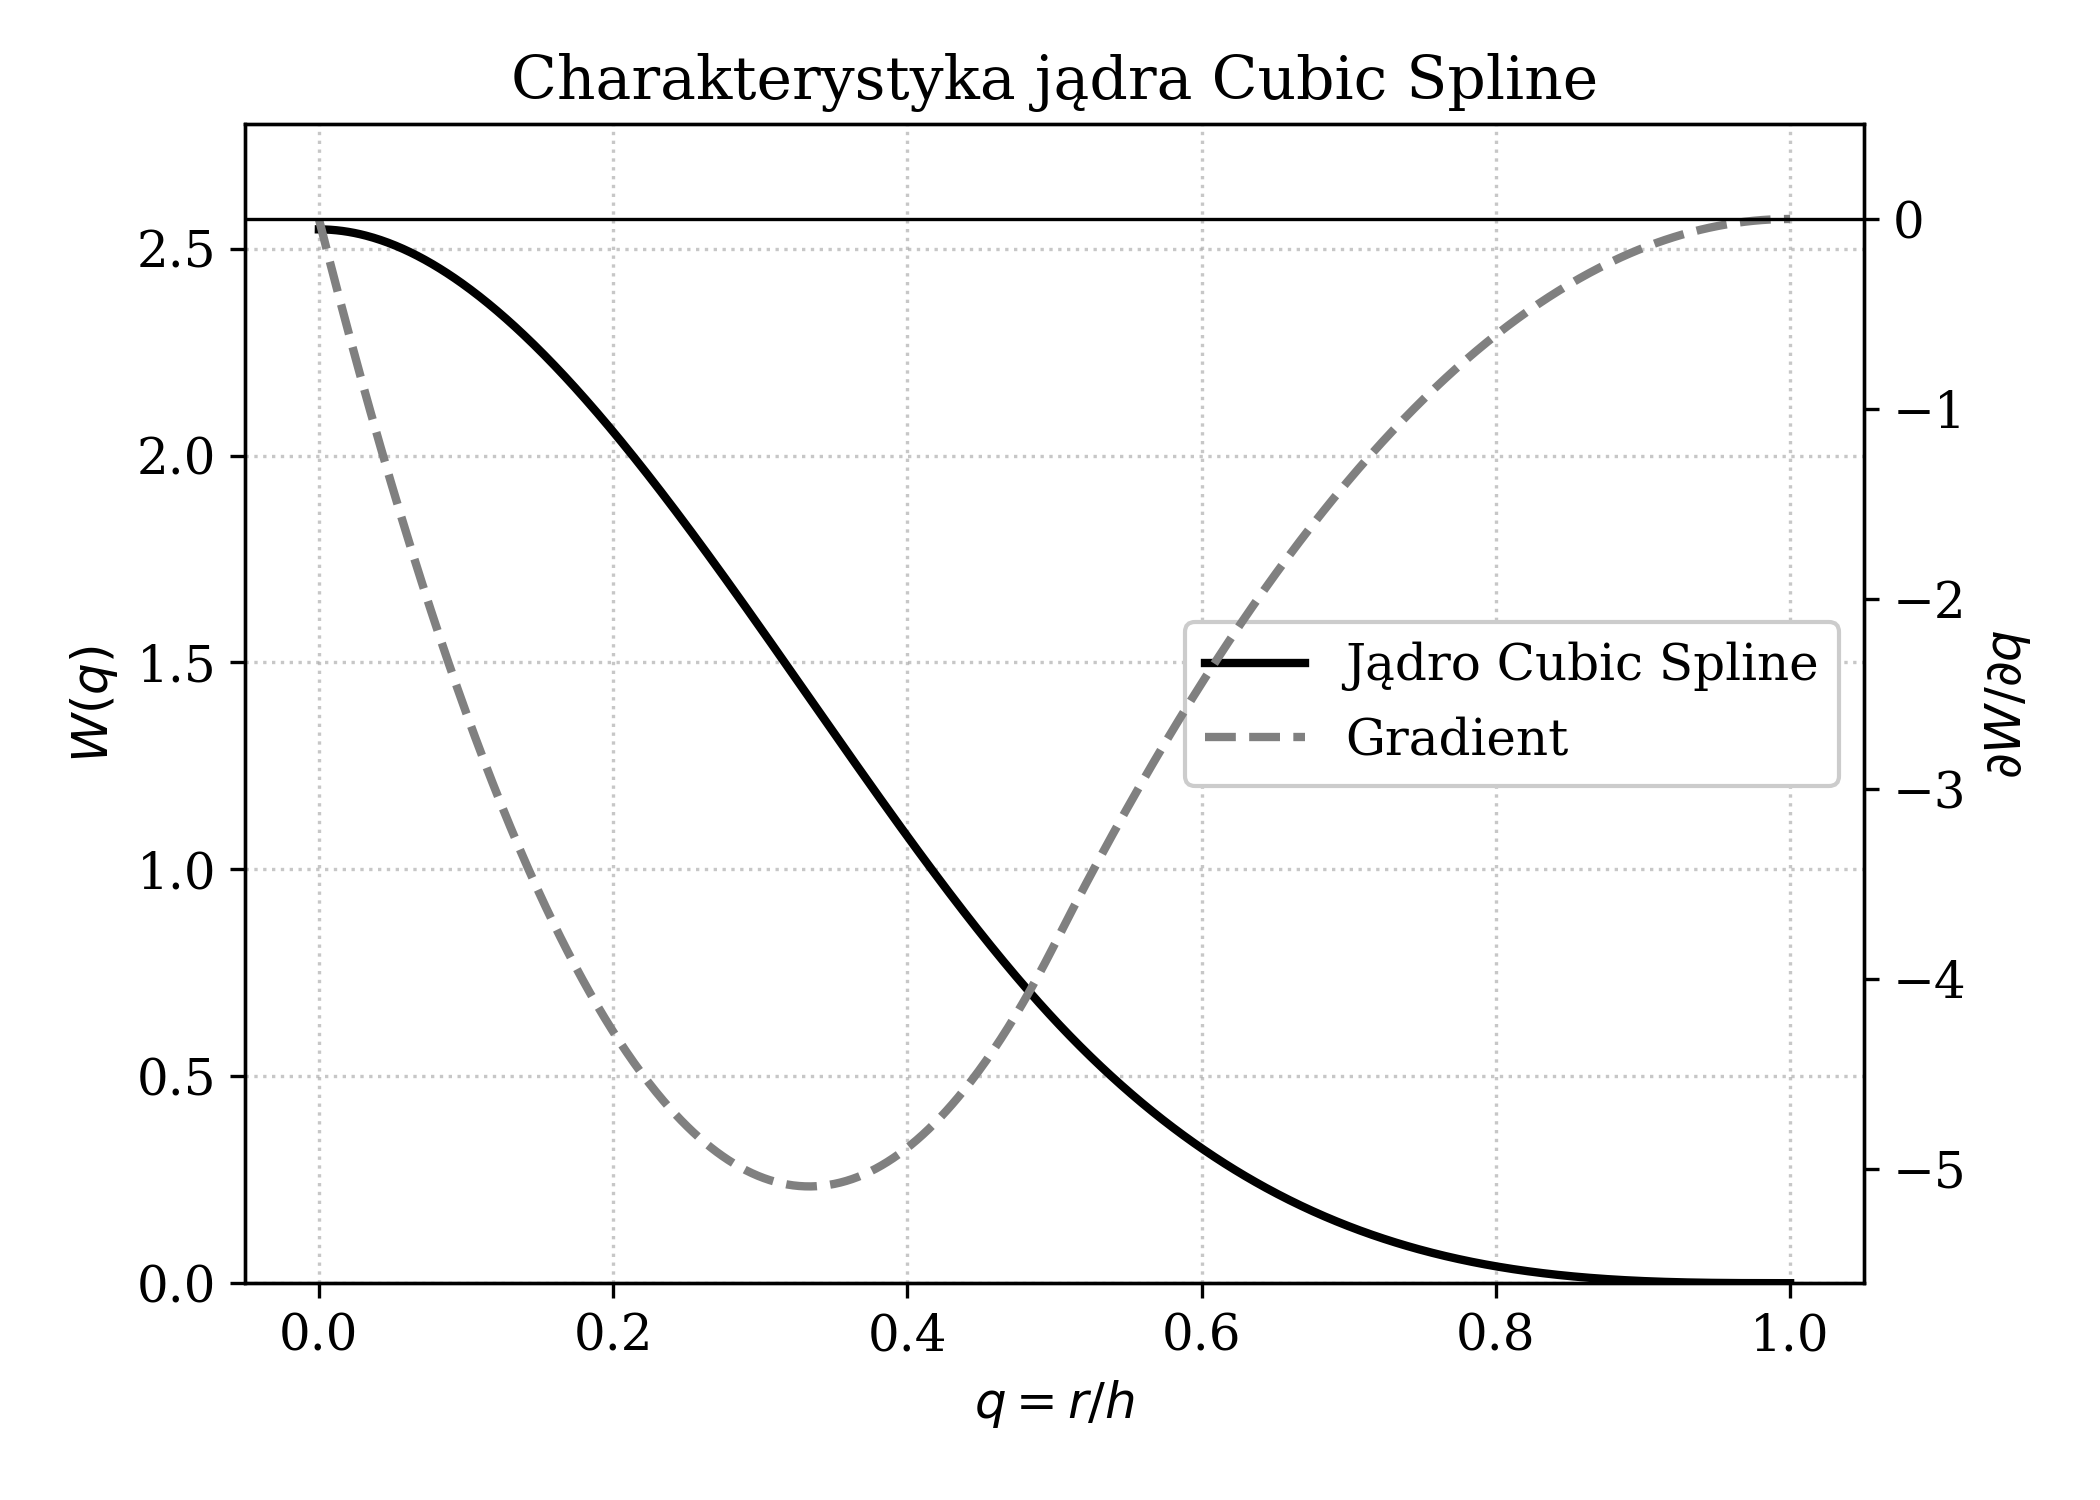
\includegraphics[width=0.72\textwidth]{figures/kernel_cubic_bw.png}
    \caption{Wartość $W(q)$ oraz pochodna radialna $\partial W/\partial q$ sześciennej
    funkcji sklejanej w~funkcji znormalizowanej odległości $q = r/h$
    \newline Źródło: Opracowanie własne na podstawie \cite{koschier2020smoothed}}
    \label{fig:kernel_cubic}
\end{figure}

\subsection{Funkcja Wendlanda C2}

Jądro Wendlanda C2 (ang.~\textit{Wendland quintic C2 kernel}) pochodzi z teorii
radialnych funkcji bazowych \cite{wendland1995piecewise}. W trójwymiarowej przestrzeni
przyjmuje postać wielomianu piątego stopnia:

\begin{equation}
    W(q,\,h) = \frac{21}{2\pi h^3}
    \begin{cases}
        (1-q)^4(4q+1) & \text{dla } 0 \leq q \leq 1, \\
        0              & \text{dla } q > 1,
    \end{cases}
    \label{eq:wendland_kernel}
\end{equation}

a jego gradient przestrzenny:

\begin{equation}
    \nabla W(\mathbf{r},\,h) = -\frac{210}{\pi h^3}
    \begin{cases}
        q(1-q)^3\,\dfrac{\mathbf{r}}{r\,h} & \text{dla } 0 < q \leq 1, \\[6pt]
        \mathbf{0}                           & \text{dla } q > 1.
    \end{cases}
    \label{eq:wendland_grad}
\end{equation}

W odróżnieniu od jądra sześciennego, funkcja Wendlanda C2 jest jednym wyrażeniem
wielomianowym na całym nośniku, bez wewnętrznych punktów sklejenia.
Posiada gwarantowaną dodatniość i monotonicznie malejący profil, a gradient zaczyna się
od zera w $q = 0$, osiąga maksimum w pewnym $q \in (0,\,1)$ i powraca do zera na granicy
nośnika, co ilustruje rysunek~\ref{fig:kernel_wendland}.

\begin{figure}[ht]
    \centering
    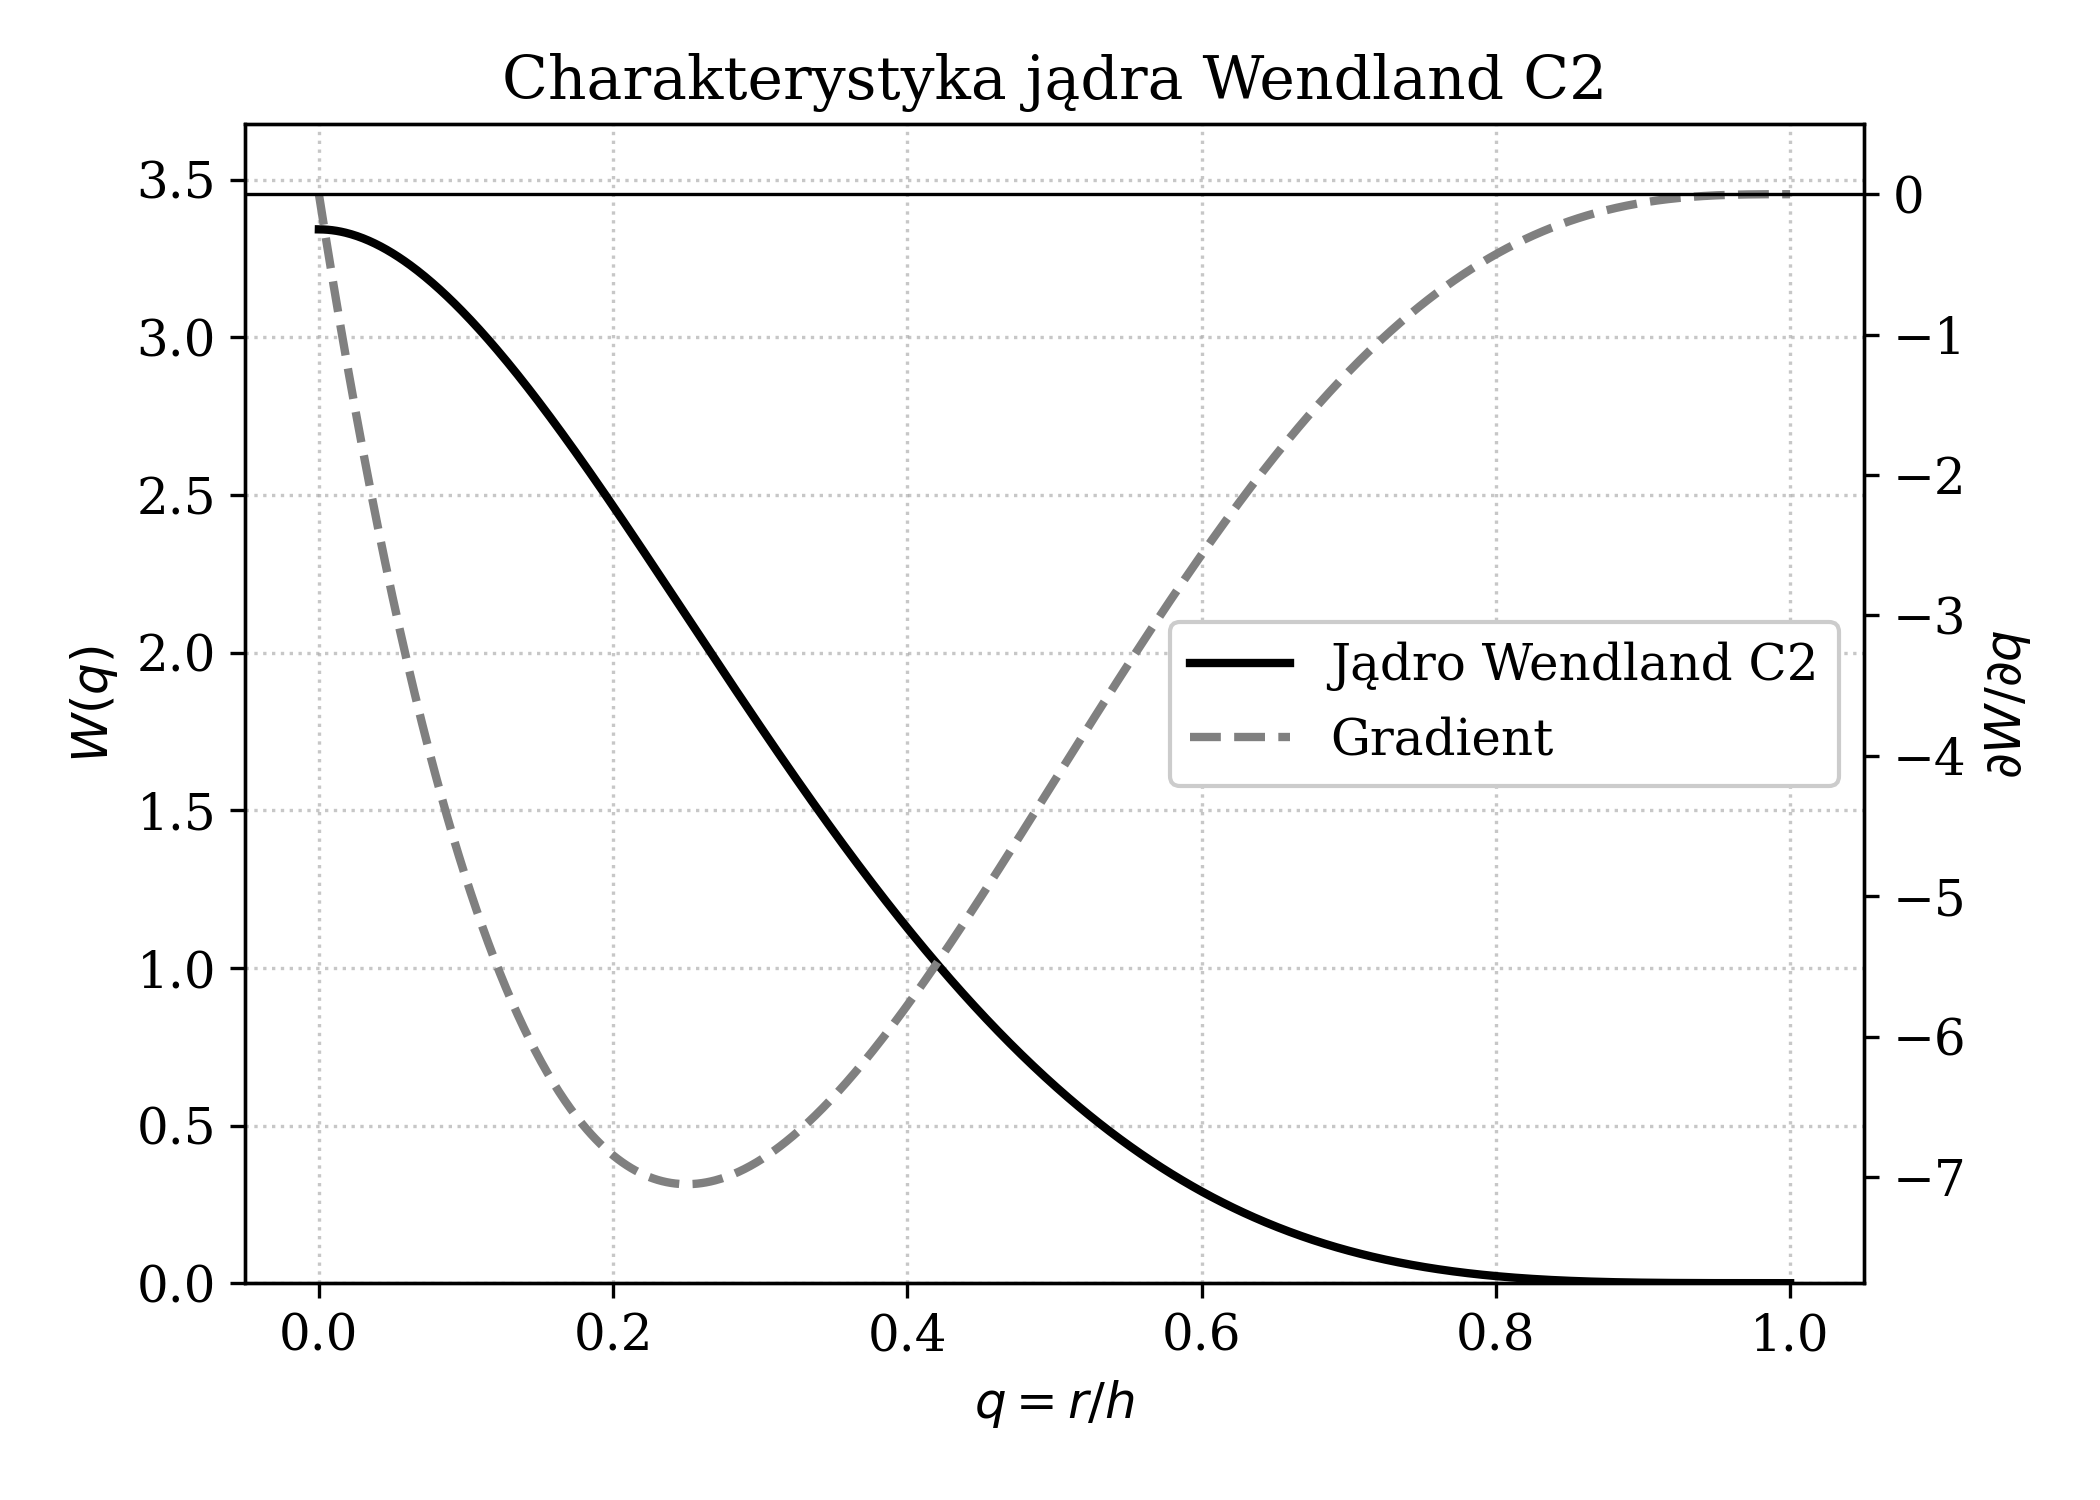
\includegraphics[width=0.72\textwidth]{figures/kernel_wendland_bw.png}
    \caption{Wartość $W(q)$ oraz pochodna radialna $\partial W/\partial q$ jądra
    Wendlanda C2 w funkcji znormalizowanej odległości $q = r/h$
    \newline Źródło: Opracowanie własne na podstawie \cite{wendland1995piecewise}}
    \label{fig:kernel_wendland}
\end{figure}

\subsection{Dobór jądra dla solvera DFSPH}

Porównując oba jądra pod kątem ich zachowania w pobliżu zera, widoczna jest zasadnicza
różnica wynikająca bezpośrednio z rysunków~\ref{fig:kernel_cubic}
i~\ref{fig:kernel_wendland}. Gradient sześciennej funkcji sklejanej jest zerowy
w punkcie $q = 0$, co oznacza, że gdy dwie cząsteczki znajdą się bardzo blisko siebie,
siła odpychająca wynikająca z jądra zanika. Prowadzi to do efektu skupiania się cząsteczek
(ang.~\textit{particle clumping}): cząsteczki, które raz do siebie nadmiernie się zbliżą,
nie napotykają wystarczającego oporu obliczeniowego i zaczynają się zagęszczać w sposób
niekontrolowany. Jądro Wendlanda C2 pozbawione jest tej wady: jego gradient rośnie
niemal liniowo od zera przy $q = 0$ i nie posiada płaskiej strefy przy początku
układu współrzędnych, co zapewnia niezerową siłę odpychającą nawet przy bardzo
małych odległościach.

Wydawałoby się to wystarczającym argumentem na korzyść jądra Wendlanda C2, jednak
badanie Lavrova i współpracowników \cite{lavrov2015density} wskazuje na istotny koszt tej
stabilności. Spośród dziesięciu analizowanych jąder SPH w przestrzeni trójwymiarowej,
jądra Wendlanda należą do grupy wymagającej największej liczby cząsteczek sąsiadujących,
aby zapewnić tę samą dokładność reprezentacji gęstości. Różnica w wymaganej liczbie
sąsiadów między jądrami sześciennymi a jądrami Wendlanda wynosi w 3D nawet trzykrotność,
przy czym kontrast ten pogłębia się wraz ze wzrostem liczby wymiarów. W implementacji
GPU, gdzie każda operacja sąsiedztwa przekłada się bezpośrednio na liczbę instrukcji
wykonywanych przez wątek obliczeniowy, szerszy nośnik efektywny jądra Wendlanda oznacza
proporcjonalnie większy koszt obliczeniowy każdego kroku symulacji.

Kluczowym argumentem przesądzającym o wyborze sześciennej funkcji sklejanej jest
właściwość algorytmu DFSPH. Solver rozbieżności, stanowiący rdzeń metody, wymusza
w każdym kroku czasowym warunek zerowej rozbieżności pola prędkości, co zapobiega
akumulacji błędów gęstości już u ich źródła. Cząsteczki nie mają możliwości nabycia
prędkości zbliżającej je do siebie na tyle, by efekt skupiania się stał się problemem,
gdyż solver koryguje prędkości zanim dojdzie do znacznego zaburzenia gęstości.
Główna słabość sześciennej funkcji sklejanej jest zatem neutralizowana przez sam
algorytm. Na zbieżność tego wniosku z praktyką wskazuje fakt, że autorzy algorytmu
DFSPH w oryginalnej publikacji \cite{bender2015divergence} sami posługują się sześcienną
funkcją sklejaną jako jądrem obliczeniowym. Warto przy tym podkreślić dodatkowe
ograniczenie wskazane przez tych samych autorów: oba solvery składające się na metodę
DFSPH, solver gęstości oraz solver rozbieżności, muszą korzystać z tej samej funkcji
wygładzającej \cite{bender2015divergence}. Oznacza to, że wybór jądra nie jest decyzją
lokalną dotyczącą jednego etapu algorytmu, lecz ma podwójny wpływ na koszt obliczeniowy
całego kroku czasowego. Wybór jądra wymagającego szerszego sąsiedztwa, jak Wendland C2,
obciążałby proporcjonalnie oba solvery jednocześnie. Wobec powyższego, w niniejszej
implementacji przyjęto sześcienną funkcję sklejaną jako jądro wygładzające, czerpiąc
korzyść z mniejszej liczby sąsiadów i tym samym niższego kosztu obliczeniowego przy
zachowaniu pełnej stabilności numerycznej gwarantowanej przez solver DFSPH.

% ----------------------------------------------------------------

\section{Wyszukiwanie sąsiedztwa cząsteczek}
\label{sec:neighbor_search_theory}

Każda cząsteczka w metodzie SPH oddziałuje wyłącznie z cząsteczkami znajdującymi się
w odległości nie większej niż promień wygładzania $h$. Poza tym promieniem wartość
jądra jest równa zero i dana para cząsteczek nie wnosi żadnego wkładu do sum
interpolacyjnych. Wyznaczenie zbioru sąsiadów jest zatem fundamentalnym krokiem
obliczeniowym wykonywanym co najmniej raz na krok czasowy, a przy iteracyjnych
solverach nieściśliwości, takich jak DFSPH, listy sąsiedztwa są wielokrotnie
odczytywane w każdej klatce.

Naiwne podejście, polegające na sprawdzeniu każdej pary cząsteczek, ma złożoność
$\mathcal{O}(N^2)$, gdzie $N$ jest liczbą cząsteczek. Dla symulacji zawierającej
$10^5$ cząsteczek oznacza to $10^{10}$ porównań na krok, co jest w praktyce
nieakceptowalne. Rozwiązaniem jest zastosowanie przestrzennej struktury danych,
które ograniczają proces wyszukiwania do najbliższego otoczenia cząsteczki, 
redukując złożoność zapytania do $\mathcal{O}(1)$ lub $\mathcal{O}(\log N)$.
Najszerzej stosowaną klasą takich struktur w metodzie SPH są siatki jednolite
(ang.~\textit{uniform grids}), których rozmiar komórki dobierany jest równy
promieniowi wygładzania $h$. Wówczas sąsiedzi danej cząsteczki mogą znajdować
się wyłącznie w~sąsiednich komórkach siatki, co w przestrzeni trójwymiarowej
ogranicza przeszukiwany obszar do co najwyżej $27$ komórek niezależnie od $N$.

\subsection{Siatka haszująca według Simona Greena}

Podejście zaproponowane przez Simona Greena \cite{green2010particle} jest
praktyczną realizacją idei siatki jednolitej przystosowaną do masowego
zrównoleglenia na GPU. Przestrzeń symulacji dzielona jest na sześcienne komórki
o boku równym $h$. Każda cząsteczka o~pozycji $\mathbf{r}_i$ przypisywana jest
do komórki o współrzędnych całkowitych:
\begin{equation}
    (k,\,l,\,m) = \left\lfloor \frac{\mathbf{r}_i}{h} \right\rfloor,
\end{equation}
a następnie te trzy współrzędne całkowite odwzorowywane są na jeden indeks tablicy
przez funkcję haszującą, co pozwala uniknąć jawnego przechowywania całej siatki
w~pamięci. Tablica haszująca przechowuje dla każdej komórki zakres indeksów
cząsteczek posortowanej tablicy cząsteczek. Budowa struktury sprowadza się do
posortowania cząsteczek według ich indeksu komórki, co na GPU realizowane jest
przez szybkie sortowanie radixowe \cite{green2010particle}.

Wyszukiwanie sąsiadów dla cząsteczki $i$ przebiega przez iterację po wszystkich
$27$ komórkach sąsiednich w trójwymiarowej siatce, pobranie odpowiednich zakresów
z tablicy haszującej i sprawdzenie warunku $\|\mathbf{r}_i - \mathbf{r}_j\| < h$
dla każdego kandydata. Schemat tej procedury ilustruje rysunek~\ref{fig:hashgrid}.

\begin{figure}[ht]
\centering
\begin{tikzpicture}[
  cell/.style={draw=black!40, thin, fill=white, minimum size=1.1cm},
  hcell/.style={draw=black!70, thin, fill=gray!18, minimum size=1.1cm},
  qcell/.style={draw=black!80, thick, fill=gray!35, minimum size=1.1cm},
  particle/.style={circle, fill=black, inner sep=0pt, minimum size=5pt},
  qparticle/.style={circle, fill=black, inner sep=0pt, minimum size=6pt},
  arr/.style={->, >=Stealth, semithick}
]
  \def\s{1.1}

  % Grid 5x5
  \foreach \c in {0,...,4} {
    \foreach \r in {0,...,4} {
      \node[cell] at (\c*\s, \r*\s) {};
    }
  }

  % Highlight 3x3 search region (cols 1-3, rows 1-3)
  \foreach \c in {1,2,3} {
    \foreach \r in {1,2,3} {
      \node[hcell] at (\c*\s, \r*\s) {};
    }
  }

  % Query cell (center)
  \node[qcell] at (2*\s, 2*\s) {};

  % Particles
  \node[particle] at (0.3, 0.2) {};
  \node[particle] at (0.7, 0.85) {};
  \node[particle] at (1.2, 0.3) {};
  \node[particle] at (1.55, 1.0) {};
  \node[particle] at (1.1, 1.5) {};
  \node[particle] at (1.75, 1.7) {};
  \node[particle] at (3.1, 1.35) {};
  \node[particle] at (2.9, 1.85) {};
  \node[particle] at (3.3, 2.5) {};
  \node[particle] at (1.3, 3.1) {};
  \node[particle] at (2.4, 3.3) {};
  \node[particle] at (3.5, 3.5) {};
  \node[particle] at (0.4, 3.8) {};
  \node[particle] at (4.2, 0.5) {};
  \node[particle] at (4.5, 2.8) {};

  % Query particle
  \node[qparticle] (qp) at (2*\s, 2*\s) {};
  \draw[black!60, dashed, thin] (qp) circle (0.95cm);

  % Labels
  \draw[arr, black!50] (2*\s, -0.18) -- (2*\s, 1.85);

  % Brace / annotation for 3x3 region
  \draw[decorate, decoration={brace, amplitude=5pt, mirror}, thick]
    (0.55, -0.6) -- (3.85, -0.6)
    node[midway, below=6pt, font=\scriptsize\sffamily] {27 komórek w 3D};
\end{tikzpicture}
\caption{Schemat wyszukiwania sąsiedztwa metodą siatki haszującej w 2D. Szare komórki
stanowią obszar przeszukiwania (w 3D odpowiada mu $3\times3\times3 = 27$ komórek).
Przerywane kółko oznacza promień wygładzania $h$; cząsteczka zapytania zaznaczona
jest w~komórce centralnej. Jedynie cząsteczki z wyróżnionych komórek są sprawdzane
pod kątem warunku $\|\mathbf{r}_i - \mathbf{r}_j\| < h$
\newline Źródło: Opracowanie własne na podstawie \cite{green2010particle}}
\label{fig:hashgrid}
\end{figure}

Metoda zapewnia złożoność budowy $\mathcal{O}(N)$ i złożoność zapytania
$\mathcal{O}(1)$ niezależną od liczby cząsteczek. Zakłada ona jednak z góry
określony rozmiar tablicy haszującej i stałą domenę symulacji, co jest
akceptowalne dla zamkniętych scen symulacyjnych.

\subsection{Skompresowane listy sąsiedztwa jako alternatywa}

Metodą stanowiącą bardziej nowoczesną alternatywę jest podejście zaproponowane
przez Banda, Gisslera i Teschnera \cite{band2019compressed}, będące wariantem
struktury połączonych list komórek (ang.~\textit{Cell-Linked-List}, CLL).
W odróżnieniu od podejścia Greena, siatka nie jest jawnie reprezentowana w
pamięci: przechowywana jest jedynie zwarta lista niepustych komórek, co eliminuje
koszt pamięciowy rzadko wypełnionych domen i umożliwia obsługę nieograniczonych
dziedzin przestrzennych bez z góry zdefiniowanego rozmiaru siatki.

Kluczowym elementem metody jest posortowanie cząsteczek według indeksu komórki
wyznaczonego krzywą Mortona, przestrzenną krzywą wypełniającą odwzorowującą
współrzędne komórki na jednowymiarowy indeks tak, by sąsiednie przestrzennie
cząsteczki trafiały do sąsiednich pozycji w tablicy. Poprawia to lokalność danych
w~pamięci podręcznej podczas iteracji po listach sąsiedztwa, co ilustruje
rysunek~\ref{fig:cll}.

\begin{figure}[ht]
\centering
\begin{tikzpicture}[
  pbox/.style={draw=black!70, fill=white, minimum width=0.72cm,
               minimum height=0.62cm, align=center, font=\scriptsize\ttfamily},
  cbox/.style={draw=black!70, fill=gray!14, minimum width=0.72cm,
               minimum height=0.62cm, align=center, font=\scriptsize\ttfamily},
  hbox/.style={draw=black!80, fill=gray!30, minimum width=0.72cm,
               minimum height=0.62cm, align=center, font=\scriptsize\ttfamily},
  arr/.style={->, >=Stealth, semithick},
  lbl/.style={font=\scriptsize\sffamily}
]
  % Sorted particle array
  \node[lbl, anchor=east] at (-0.4, 1.5) {cząsteczki};
  \foreach[count=\i from 0] \c in {2,2,3,3,3,5,5,7,7,7,7,9} {
    \pgfmathsetmacro{\ishigh}{(\c==3||(\c==7)) ? 1 : 0}
    \ifnum\c=3
      \node[hbox] at (\i*0.74, 1.5) {\i};
    \else
      \ifnum\c=7
        \node[hbox] at (\i*0.74, 1.5) {\i};
      \else
        \node[pbox] at (\i*0.74, 1.5) {\i};
      \fi
    \fi
  }

  % Cell indices below
  \node[lbl, anchor=east] at (-0.4, 0.75) {komórka};
  \foreach[count=\i from 0] \c in {2,2,3,3,3,5,5,7,7,7,7,9} {
    \ifnum\c=3
      \node[hbox] at (\i*0.74, 0.75) {\c};
    \else
      \ifnum\c=7
        \node[hbox] at (\i*0.74, 0.75) {\c};
      \else
        \node[cbox] at (\i*0.74, 0.75) {\c};
      \fi
    \fi
  }

  % Compact cell array
  \node[lbl, anchor=east] at (-0.6, -0.1) {zwarta lista komórek};
  \foreach[count=\i from 0] \entry in {{2:0},{3:2},{5:5},{7:7},{9:11}} {
    \node[cbox, minimum width=1.3cm] at (\i*1.36, -0.1) {\entry};
  }

  \node[lbl, anchor=west] at (6.95, 1.5) {\dots};
  \node[lbl, anchor=west] at (6.95, 0.75) {\dots};

  \node[lbl, font=\scriptsize\itshape] at (3.4, -0.65)
    {format: indeks\_komórki : pierwszy\_indeks\_cząsteczki};
\end{tikzpicture}
\caption{Schemat struktury CLL z kompaktową tablicą komórek. Górny wiersz zawiera
indeksy cząsteczek posortowane według indeksu komórki (wyznaczonego krzywą Mortona);
środkowy wiersz pokazuje odpowiadające indeksy komórek; dolny wiersz przedstawia
zwartą tablicę komórek przechowującą wyłącznie niepuste komórki z odniesieniem do
pierwszej cząsteczki w posortowanej tablicy. Wyróżnione (szare) pola odpowiadają
przykładowym komórkom 3 i 7
\newline Źródło: Opracowanie własne na podstawie \cite{band2019compressed}}
\label{fig:cll}
\end{figure}

Drugą cechą wyróżniającą metodę jest kompresja list sąsiedztwa. Ponieważ
cząsteczki są posortowane, indeksy sąsiadów są niemalejące, a ich różnice
są małe. Autorzy wykorzystują tę właściwość, kodując różnice kolejnych
indeksów sąsiadów za pomocą schematu inspirowanego algorytmem StreamVByte,
osiągając oszczędność pamięci sięgającą $87\%$ w porównaniu z nieskompresowaną
reprezentacją. W iteracyjnych solverach nieściśliwości, takich jak DFSPH,
gdzie listy sąsiedztwa są wielokrotnie odczytywane w każdym kroku, przechowywanie
skompresowanych list i ich odczytywanie na żądanie jest naturalnym rozwiązaniem.
Metoda ta jest szczególnie korzystna dla dużych symulacji w otwartych scenach,
gdzie domena nie jest z góry ograniczona, a siatka haszująca wymagałaby rozbudowanej
tablicy. Jej implementacja opisana w \cite{band2019compressed} jest ukierunkowana
na procesory wielordzeniowe; autorzy wskazują implementację GPU jako kierunek
dalszych badań. Z tego względu, przy implementacji opartej w całości na GPU,
zastosowano prostsze podejście siatki haszującej opisane w podrozdziale poprzednim.

% ----------------------------------------------------------------

\section{Modelowanie zjawisk fizycznych}
\label{sec:physical_models_theory}

Równanie pędu Naviera-Stokesa zawiera trzy człony siłowe: gradient ciśnienia,
naprężenia lepkie oraz siły zewnętrzne. Solver DFSPH, opisany w poprzednich
rozdziałach, rozwiązuje wyłącznie człon ciśnieniowy, wymuszając nieściśliwość.
Pozostałe zjawiska fizyczne, mianowicie opór lepki, kohezja cząsteczek na
powierzchni swobodnej oraz oddziaływanie z granicami domeny, wymagają osobnych
modeli dyskretnych. Każde z nich może być pominięte w minimalnej implementacji
solvera, lecz każde odpowiada za inny aspekt fizycznej poprawności symulacji.
W niniejszej sekcji omówiono teoretyczne podstawy tych modeli.

\subsection{Lepkość}

Lepkość jest miarą wewnętrznego oporu cieczy na odkształcenie ścinające. W równaniu
pędu odpowiada za nią tensor naprężeń dewiacyjnych $\boldsymbol{\tau}$. Dla cieczy
newtonowskich tensor ten jest proporcjonalny do symetrycznego gradientu prędkości:
\begin{equation}
    \boldsymbol{\tau} = \mu \left( \nabla \mathbf{u} + (\nabla \mathbf{u})^\top \right),
\end{equation}
gdzie $\mu$ jest dynamicznym współczynnikiem lepkości. Dywergencja tego tensora
wchodzi do równania pędu jako przyspieszenie lepkie $\mathbf{a}^{\mathrm{visc}}$.
W dyskretyzacji SPH najczęściej stosowanym podejściem jest sformułowanie Morrisa
i współpracowników \cite{morris1997modeling}, które zastępuje człon
$\nabla \cdot \boldsymbol{\tau}$ operatorem opartym na laplasjanie prędkości:
\begin{equation}
    \mathbf{a}^{\mathrm{visc}}_i = \frac{\mu}{\rho_i}
    \sum_j \frac{m_j}{\rho_j} \, (\mathbf{v}_j - \mathbf{v}_i)
    \frac{1}{r_{ij}} \frac{\partial W_{ij}}{\partial r},
\end{equation}
gdzie $r_{ij} = \|\mathbf{r}_i - \mathbf{r}_j\|$. Wyraz ten tłumi względne
prędkości sąsiadów proporcjonalnie do odległości, modelując dyssypację energii
kinetycznej charakterystyczną dla cieczy lepkich. Brak członu lepkiego sprawia,
że ciecz zachowuje się jak idealna, zachowując energię mechaniczną bez strat,
co jest fizycznie nierealistyczne dla większości cieczy, choć nie destabilizuje
solvera.

Odrębnym mechanizmem pokrewnym lepkości jest korekcja XSPH \cite{monaghan1989problem},
w której prędkość cząsteczki jest nieznacznie uśredniana względem prędkości jej
sąsiadów. Nie modeluje ona jawnie dyssypacji energii, lecz wygładza pole prędkości,
zapobiegając przenikaniu i lokalnym skupieniom cząsteczek. Mechanizm ten działa
niezależnie od fizycznej lepkości i może być stosowany zarówno przy $\mu = 0$,
jak i przy niezerowej jej wartości.

\subsection{Napięcie powierzchniowe}

Napięcie powierzchniowe jest efektem makroskopowym niezrównoważonych sił kohezji
działających na cząsteczki cieczy leżące przy granicy fazy swobodnej. Cząsteczka
w głębi cieczy jest otoczona sąsiadami ze wszystkich stron i suma sił kohezji
znosi się; cząsteczka na powierzchni ma sąsiadów tylko po stronie cieczy, co
wytwarza wypadkową siłę skierowaną do jej wnętrza. Efektem jest minimalizacja
pola powierzchni swobodnej i charakterystyczny kształt kropli.

W sformułowaniu opartym na równaniu Younga-Laplace'a \cite{batchelor1967introduction}
różnica ciśnienia po obu stronach zakrzywionej powierzchni wynosi:
\begin{equation}
    \Delta p = \gamma \kappa,
\end{equation}
gdzie $\gamma$ jest współczynnikiem napięcia powierzchniowego, a $\kappa$ krzywizną
powierzchni. W metodzie SPH krzywizna wyznaczana jest na podstawie pola normalnego
szacowanego z gradientu jądra, a wypadkowa siła kohezji przykładana jest jako
przyspieszenie cząsteczek leżących przy powierzchni. Bez napięcia powierzchniowego
symulacja pozostaje stabilna, lecz traci zdolność do formowania kropli i
realistycznego zachowania cienkiej warstwy cieczy. W niniejszej pracy napięcie
powierzchniowe nie zostało zaimplementowane; symulowane sceny obejmują swobodną
powierzchnię bez zjawisk kapilarnych, gdzie jego pominięcie nie wpływa istotnie
na poprawność wyników \cite{koschier2020smoothed}.

\subsection{Warunki brzegowe}

Granice domeny symulacji wprowadzają fundamentalny problem geometryczny: cząsteczka
znajdująca się w pobliżu ściany ma niepełny obszar wsparcia jądra, ponieważ część
sfery sąsiedztwa o promieniu $h$ wychodzi poza domenę i nie zawiera żadnych
cząsteczek. Sytuację tę ilustruje rysunek~\ref{fig:boundary_support}.

\begin{figure}[ht]
\centering
\begin{tikzpicture}[scale=1.3,
  particle/.style={circle, fill=black, inner sep=0pt, minimum size=5pt},
  ghost/.style={circle, draw=black!40, fill=gray!15, inner sep=0pt,
                minimum size=5pt, dashed},
  arr/.style={->, >=Stealth, semithick}
]
  % Wall (hatch fill)
  \fill[gray!20] (-0.5, -0.5) rectangle (0.5, 2.5);
  \draw[thick] (0.5, -0.5) -- (0.5, 2.5);
  \foreach \y in {-0.3, 0.1, 0.5, 0.9, 1.3, 1.7, 2.1} {
    \draw[black!30, thin] (0.1, \y) -- (0.5, \y+0.4);
  }
  \node[font=\scriptsize\sffamily, rotate=90] at (0.0, 1.0) {ściana};

  % Query particle
  \node[particle, fill=black] (qp) at (1.3, 1.0) {};
  \node[font=\scriptsize\sffamily, above=3pt] at (qp) {$i$};

  % Support radius circle
  \draw[black, dashed, thin] (qp) circle (1.2cm);
  \node[font=\scriptsize\sffamily] at (2.6, 1.85) {$h$};

  % Fluid particles (only on fluid side)
  \node[particle] at (1.7, 0.3) {};
  \node[particle] at (2.1, 1.1) {};
  \node[particle] at (1.6, 1.7) {};
  \node[particle] at (2.3, 0.6) {};
  \node[particle] at (1.9, 1.7) {};

  % Missing region annotation
  \draw[black!50, thin, <->] (0.5, -0.3) -- (1.3, -0.3)
    node[midway, below, font=\scriptsize\sffamily] {brak sąsiadów};

  % Ghost particles (mirror)
  \node[ghost] at (0.9, 0.3) {};
  \node[ghost] at (0.5, 1.0) {};
  \node[ghost] at (0.9, 1.7) {};
  \node[font=\scriptsize\sffamily, black!50] at (-0.1, 0.4)
    {\textit{duch}};
\end{tikzpicture}
\caption{Problem niepełnego sąsiedztwa przy granicy domeny. Sfera wsparcia
cząsteczki $i$ przecina ścianę; brak sąsiadów po lewej stronie prowadzi do
zaniżenia oszacowania gęstości i błędu gradientu ciśnienia. Cząsteczki-duchy
(szare, przerywane) uzupełniają brakujący obszar wsparcia
\newline Źródło: Opracowanie własne na podstawie \cite{schechter2012ghost}}
\label{fig:boundary_support}
\end{figure}

Konsekwencje niekompletnego sąsiedztwa są wielorakie. Gęstość wyznaczana sumą
SPH jest zaniżona względem wartości spoczynkowej $\rho_0$, co powoduje, że solver
ciśnienia generuje w pobliżu ścian fałszywy gradient przyciągający cząsteczki do
granicy. Gradient ciśnienia jest dodatkowo błędnie skierowany, ponieważ suma
po sąsiadach nie jest symetrycznie rozkładana wokół cząsteczki. Przy dużych
krokach czasowych możliwe jest też przenikanie cząsteczek przez ścianę.

Powszechnym rozwiązaniem w literaturze są cząsteczki-duchy \cite{schechter2012ghost},
tworzone symetrycznie po drugiej stronie granicy jako odbicia cząsteczek fluidu.
Uzupełniają one brakujący obszar wsparcia, przywracając symetrię sumy SPH, i mogą
być wyposażone w odwróconą prędkość normalną, modelując sprężyste lub lepkie odbicie
od ściany. Alternatywą są stałe warstwy cząsteczek brzegowych reprezentujące
geometrię przeszkody, których cząsteczki uczestniczą w sumach SPH, lecz nie podlegają
integracji ruchu. W niniejszej pracy zastosowano uproszczone podejście: po każdym
kroku całkowania pozycja cząsteczek przekraczających granicę domeny jest korygowana
do jej wnętrza, a składowa normalna prędkości jest odbijana.

% ----------------------------------------------------------------

\section{Potok wizualizacji}
\label{sec:visualization_pipeline_theory}

Wynikiem każdego kroku symulacji DFSPH jest zbiór $N$ cząsteczek z~zaktualizowanymi
pozycjami. Cząsteczki stanowią dyskretne punkty masy; same w sobie nie tworzą
żadnej ciągłej powierzchni, którą mógłby przetworzyć renderer. Aby uzyskać
fotorealistyczny obraz cieczy, potok wizualizacji wykonuje trzy kolejne etapy:
rekonstrukcję ciągłego pola gęstości ze zbioru punktów, wyznaczenie niejawnej
izopowierzchni metodą raymarching oraz obliczenie koloru piksela z~uwzględnieniem
fizycznych właściwości optycznych wody. Ogólną strukturę potoku ilustruje
rysunek~\ref{fig:vis_pipeline}.

\begin{figure}[ht]
\centering
\begin{tikzpicture}[
  box/.style={rectangle, draw=black, thick, rounded corners=3pt,
              minimum width=2.6cm, minimum height=0.85cm,
              font=\small\sffamily, align=center, inner sep=5pt},
  arr/.style={->, >=Stealth, thick}
]
  \node[box] (sim) at (0,    0)   {Cząsteczki\\SPH};
  \node[box] (spl) at (3.6,  0)   {Splatting\\(siatka wokseli)};
  \node[box] (tex) at (7.2,  0)   {3D tekstura\\gęstości};
  \node[box] (ray) at (10.8, 0)   {Raymarching\\(izopowierzchnia)};
  \node[box] (shd) at (10.8,-2.0) {Model\\optyczny};
  \node[box] (px)  at (7.2, -2.0) {Kolor\\piksela};
  \draw[arr] (sim) -- (spl);
  \draw[arr] (spl) -- (tex);
  \draw[arr] (tex) -- (ray);
  \draw[arr] (ray) -- (shd);
  \draw[arr] (shd) -- (px);
\end{tikzpicture}
\caption{Potok wizualizacji: od listy cząsteczek SPH do końcowego koloru piksela
\newline Źródło: Opracowanie własne}
\label{fig:vis_pipeline}
\end{figure}

\subsection{Rekonstrukcja pola gęstości}

Pierwszym krokiem potoku jest przekształcenie listy pozycji cząsteczek w~trójwymiarową
teksturę wolumetryczną \cite{kaufman2005overview}. Domenę symulacji dzieli się na
regularną siatkę wokseli o~rozdzielczości $G_x \times G_y \times G_z$, gdzie każdy
woksel przechowuje skumulowaną gęstość wyrażoną liczbą całkowitą. Dla każdej
cząsteczki $i$ wyznaczany jest odpowiadający jej woksel centralny $\mathbf{c}_i$,
a~następnie do każdego woksela $\mathbf{c}$ w promieniu $R$ wokseli dodawana jest
waga:
\begin{equation}
    w(\delta) = \left(1 - \left(\frac{\delta}{R}\right)^{\!2}\right)^{\!3},
    \qquad \delta = \|\mathbf{c} - \mathbf{c}_i\|.
    \label{eq:splat_weight}
\end{equation}
Funkcja ta jest gładkim wielomianem wygasającym do zera na granicy kuli, co
gwarantuje ciągłość pola bez nieciągłości widocznych jako artefakty wizualne.

Ponieważ każda cząsteczka przetwarzana jest przez osobny wątek GPU, wiele wątków
może jednocześnie aktualizować ten sam woksel. Konflikty zapisu rozwiązuje
instrukcja atomowa \texttt{imageAtomicAdd}, która gwarantuje spójność sumy bez
konieczności synchronizacji. Wynikiem etapu splatting jest trójwymiarowa tekstura
liczb całkowitych: woksele wewnątrz masy cieczy osiągają wartości rzędu setek,
woksele powietrza zbliżone są do zera. Granica między tymi obszarami stanowi
niejawną definicję powierzchni cieczy.

\subsection{Raymarching izopowierzchni}

Mając pole gęstości $\rho(\mathbf{p})$ zapisane w~teksturze 3D, powierzchnię
cieczy definiuje się jako izopowierzchnię:
\begin{equation}
    S = \bigl\{\,\mathbf{p} \in \mathbb{R}^3 : \rho(\mathbf{p}) = \rho_{\mathrm{thr}}\,\bigr\}.
\end{equation}
Wyznaczenie przecięcia promienia kamery z~tą powierzchnią realizuje metoda
raymarching \cite{quilez2008raymarching, tomczak2012gpu}: promień emitowany ze
środka projekcji przemieszcza się równomiernymi krokami $\Delta t$ wzdłuż swojego
kierunku, w każdym punkcie próbkując teksturę, aż wartość gęstości przekroczy próg.
Przed rozpoczęciem marszowania wykonywany jest test przecięcia promienia
z~prostopadłościanem wyrównanym do osi (ang.~\textit{Axis-Aligned Bounding Box}, AABB), czyli
minimalnym prostopadłościanem wyrównanym do osi układu współrzędnych,
który szczelnie otacza domenę symulacji. Test ten, oparty na metodzie płaszczyzn
równoległych, wyznacza w~sposób analityczny zakres
parametru $t \in [t_{\min},\, t_{\max}]$ odpowiadający wejściu i~wyjściu promienia
z~domeny; promienie nie trafiające w~AABB odrzucane są na poziomie shadera
fragmentów, zanim pętla marszowania w~ogóle się rozpocznie.

Próbkowanie tekstury odbywa się z~ręczną interpolacją trójliniową ośmiu sąsiednich
tekseli, zapewniającą ciągłość sygnału niezbędną do poprawnego wyliczenia normalnych.
Aby uniknąć pominięcia cienkiej warstwy cieczy przy dużym kroku, po wykryciu
pierwszego przekroczenia progu wykonuje się ośmiokrotną bisekcję przedziału
$[t_{\mathrm{prev}},\, t_{\mathrm{hit}}]$, lokalizując punkt powierzchni z~dokładnością
$\Delta t\,/\,2^8$ bez zmniejszania globalnego kroku. Schemat algorytmu ilustruje
rysunek~\ref{fig:raymarching}.

\begin{figure}[ht]
\centering
\begin{tikzpicture}[scale=1.05,
  miss/.style={circle, draw=black, fill=white, inner sep=0pt, minimum size=7pt},
  hit/.style={circle, fill=black!55, inner sep=0pt, minimum size=7pt}
]
  % Fluid blob (ellipse, left edge at x = 5.8 - 1.9 = 3.9)
  \fill[gray!15] (5.8, 0) ellipse (1.9cm and 1.1cm);
  \draw[thick]   (5.8, 0) ellipse (1.9cm and 1.1cm);
  \node[font=\scriptsize\sffamily, gray!70] at (5.8, 0) {ciecz};
  \node[font=\scriptsize\sffamily] at (2.0, 1.3) {izopowierzchnia};
  \draw[->, gray!60, thin] (2.65, 1.2) -- (3.65, 0.6);

  % Camera
  \filldraw[black] (-0.2, 0) circle (2.5pt);
  \node[font=\footnotesize\sffamily, below=3pt] at (-0.2,0) {kamera};

  % Ray
  \draw[->, >=Stealth, thick] (-0.2, 0) -- (8.2, 0)
    node[right, font=\scriptsize\sffamily] {promień};

  % Miss samples (x < 3.9)
  \node[miss] at (0.8, 0) {};
  \node[miss] at (1.7, 0) {};
  \node[miss] at (2.6, 0) {};
  \node[miss] at (3.5, 0) {};
  \node[font=\scriptsize\sffamily, above=4pt] at (3.5, 0) {$t_4$};

  % Hit sample (x = 4.4, inside ellipse since 4.4 > 3.9)
  \node[hit] at (4.4, 0) {};
  \node[font=\scriptsize\sffamily, above=4pt] at (4.4, 0) {$t_5$};

  % Binary search bracket
  \draw[<->, >=Stealth, gray, semithick] (3.5,-0.52) -- (4.4,-0.52)
    node[midway, below, font=\scriptsize\sffamily, gray] {bisekcja $\times 8$};

  % True surface point (left edge of ellipse at x=3.9)
  \draw[dashed, black!40] (3.9,-0.72) -- (3.9, 0.65);
  \filldraw[black] (3.9, 0) circle (2.5pt);
  \node[font=\scriptsize\sffamily, above=4pt] at (3.9, 0) {$\mathbf{p}_s$};

  % Normal arrow
  \draw[->, >=Stealth, thick] (3.9, 0) -- (3.0, 0.75)
    node[above left, font=\scriptsize\sffamily] {$\mathbf{N}$};
\end{tikzpicture}
\caption{Schemat raymarchingu z~binarnym zawężaniem. Białe kółka to próbki poniżej
         progu gęstości (powietrze), szare kółko to pierwsza próbka powyżej progu
         (ciecz). Bisekcja przedziału $[t_4,\, t_5]$ wyznacza punkt powierzchni
         $\mathbf{p}_s$ z~dokładnością $\Delta t / 2^8$
         \newline Źródło: Opracowanie własne na podstawie \cite{quilez2013advancing}}
\label{fig:raymarching}
\end{figure}

Normalna powierzchni wyznaczana jest metodą różnic skończonych na polu gęstości~\cite{tomczak2012gpu}:
\begin{equation}
    \mathbf{N}(\mathbf{p}) = -\,\nabla\rho(\mathbf{p}) \approx -\frac{1}{2\varepsilon}
    \begin{pmatrix}
        \rho(\mathbf{p}+\varepsilon\hat{x}) - \rho(\mathbf{p}-\varepsilon\hat{x}) \\[2pt]
        \rho(\mathbf{p}+\varepsilon\hat{y}) - \rho(\mathbf{p}-\varepsilon\hat{y}) \\[2pt]
        \rho(\mathbf{p}+\varepsilon\hat{z}) - \rho(\mathbf{p}-\varepsilon\hat{z})
    \end{pmatrix}.
\end{equation}
Podejście to nie wymaga jawnej siatki trójkątów i~automatycznie odzwierciedla
bieżącą topologię pola gęstości, co jest kluczowe przy dynamicznie zmieniającej
się powierzchni cieczy.

\subsection{Model optyczny cieczy}

Woda jest dielektrycznym, częściowo transparentnym ośrodkiem, w~którym na powierzchni
jednocześnie zachodzi odbicie i~załamanie światła, a~wewnątrz objętości promienie
ulegają absorpcji i~rozproszeniu \cite{pharr2016physically}. Poniżej omówiono kolejno
efekty zaimplementowane w~shaderze fragmentów.

\textbf{Środowisko HDRI.} Otoczenie sceny reprezentuje sferyczna mapa środowiskowa
w~formacie równokątnym (ang.~\textit{equirectangular}), próbkowana przez osobny shader
nieba. Każde odbicie i~załamanie na powierzchni wody próbkuje tę samą teksturę
w~przeliczonym kierunku, zapewniając spójność oświetlenia między cieczą a~tłem.

\textbf{Efekt Fresnela.} Stosunek energii odbitej do załamanej zależy od kąta
padania i~właściwości dielektrycznych ośrodka \cite{de2006reflections}. Dla wody
o~współczynniku załamania $n = 1{,}333$ odbicie przy normalnym kącie padania wynosi:
\begin{equation}
    F_0 = \left(\frac{n_1 - n_2}{n_1 + n_2}\right)^{\!2} \approx 0{,}02
\end{equation}
i~wzrasta do jedności przy kącie ślizgowym. W~shaderze stosuje się przybliżenie
Schlicka:
\begin{equation}
    F(\theta) = F_0 + (1 - F_0)(1 - \cos\theta)^5,
\end{equation}
gdzie $\theta$ jest kątem między wektorem widoku $\mathbf{V}$ a~normalną $\mathbf{N}$.
Kierunek odbitego promienia próbkuje skybox, kierunek załamanego wyznaczany jest
prawem Snella. Końcowy kolor piksela to interpolacja liniowa między kolorem
załamania a~odbicia z~wagą $F$.

\textbf{Absorpcja Beer-Lamberta.} Światło przenikające przez grubość cieczy $d$
ulega wykładniczej absorpcji:
\begin{equation}
    \mathbf{c}_{\mathrm{abs}} = \mathbf{c}_{\mathrm{bg}} \cdot
    \exp(-\boldsymbol{\mu}_a \cdot d),
\end{equation}
gdzie $\boldsymbol{\mu}_a = (\mu_R,\, \mu_G,\, \mu_B)$ są kanałowymi współczynnikami
absorpcji. Silna absorpcja czerwonego ($\mu_R = 0{,}45$) przy słabej niebieskiego
($\mu_B = 0{,}025$) nadaje wodzie charakterystyczną niebieskozieloną barwę.
Grubość $d$ wyznaczana jest osobnym przebiegiem promienia od punktu powierzchni
do tylnej ściany AABB.

\textbf{Rozproszenie podpowierzchniowe.} Część energii słonecznej nie jest
pochłaniana, lecz wielokrotnie rozpraszana wewnątrz cieczy i~wychodzi jako miękka
turkusowa poświata widoczna zwłaszcza w~cienkich partiach fali. Efekt modeluje się
przybliżeniem łączącym zawiniętą dyfuzję (ang.~\textit{wrapped diffuse}) z~tylnym
rozproszeniem:
\begin{equation}
    L_{\mathrm{sss}} = c_s \cdot L_{\odot} \cdot
    \bigl(0{,}6\;\sigma_{\mathrm{wrap}} + 0{,}4\;\sigma_{\mathrm{back}}\bigr)
    \cdot \bigl(1 - e^{-3d}\bigr),
\end{equation}
gdzie $\sigma_{\mathrm{wrap}} = \max\bigl(0,\,\mathbf{N}{\cdot}\mathbf{L}\cdot0{,}5+0{,}5\bigr)$
modeluje oświetlenie przechodzące przez krawędź fali, a~$\sigma_{\mathrm{back}} =
\max(0,\,-\mathbf{N}{\cdot}\mathbf{L})$ odpowiada za tylne rozproszenie w~kierunku
obserwatora.

\textbf{Odbłysk spekularny GGX.} Mikrostruktury falującej powierzchni modeluje
rozkład normalnych GGX \cite{walter2007microfacet} o~parametrze szerokości $\alpha = 0{,}04$:
\begin{equation}
    D_{\mathrm{GGX}}(\mathbf{H}, \alpha) =
    \frac{\alpha^2}{\pi\,\bigl[(\mathbf{N}{\cdot}\mathbf{H})^2(\alpha^2-1)+1\bigr]^2},
\end{equation}
gdzie $\mathbf{H} = \mathrm{normalize}(\mathbf{L} + \mathbf{V})$ jest półwektorem
między kierunkiem światła a~wektorem widoku, a~$\alpha$~--- parametrem szerokości
rozkładu GGX odpowiadającym chropowatości powierzchni.

\textbf{Piana i~mapowanie tonalne.} Regiony, w~których normalna jest prawie pionowa
($N_y \approx 1$) przy małej grubości cieczy, maskowane są kolorem pianki,
naśladując bąble powietrza na grzbietach fali. Na koniec kolor HDR przekształcany
jest operatorem Reinharda \cite{reinhard2002photographic}
$\mathbf{c}' = \mathbf{c}\,/\,(1+\mathbf{c})$ do zakresu $[0,1]$ przed zapisem
do bufora ramki.


\chapter{Implementacja i oryginalne rozwiązania techniczne}
% ============================================================
% Rozdział 3 — Implementacja i oryginalne rozwiązania techniczne
% Plan: docs/chapter3_plan.md
% ============================================================

Przejście od matematycznego opisu dynamiki cieczy do działającej implementacji
obliczeniowej jest samo w sobie wyzwaniem inżynierskim. Równania różniczkowe
opisujące zachowanie cieczy są precyzyjne i eleganckie; ich dyskretyzacja oraz
wykonanie na rzeczywistym sprzęcie odsłaniają natomiast ograniczenia, które
w modelu teoretycznym nie istnieją. Każdy krok symulacji musi zostać
zdekomponowany na operacje równoległe wykonywane przez tysiące wątków GPU,
a ta równoległość niesie ze sobą nowe klasy problemów nieobecne w algorytmach
sekwencyjnych: równoczesny odczyt i zapis buforów, konieczność koherencji
pamięci podręcznej, wrażliwość na wzorzec dostępu do pamięci globalnej.

Implementacja w modelu GPGPU (ang.~\textit{General-Purpose computing on Graphics Processing Units}) 
nie jest przepisaniem algorytmu sekwencyjnego
na kod shaderów. Wymaga świadomego projektowania struktur danych pod kątem
przepustowości pamięci, doboru algorytmów sortowania dostosowanych do
architektury SIMT (ang.~\textit{Single Instruction, Multiple Threads}), 
zarządzania synchronizacją między etapami potoku
obliczeniowego oraz kontroli arytmetyki zmiennoprzecinkowej, której błędy
akumulacji mogą zdestabilizować pozornie poprawną symulację.

Niniejszy rozdział przedstawia implementację silnika symulacji cieczy opartego
na metodzie DFSPH, realizowanej na GPU, w formie ciągu wyzwań i kompromisów
technicznych. Każda decyzja projektowa --- od wyboru struktury danych
i algorytmu sortowania, przez strategię doboru kroku czasowego, po architekturę
potoku renderowania --- jest uzasadniona analizą strukturalną lub bezpośrednim
pomiarem.

% ------------------------------------------------------------
\section{Założenia projektowe}
\label{sec:assumptions}

Uruchomienie silnika wymaga spełnienia wymagań sprzętowych i programowych
opisanych poniżej. Projekt jest przeznaczony wyłącznie dla systemu Windows ---
kod źródłowy korzysta z rozszerzenia \texttt{winit::platform::windows}, które
udostępnia funkcjonalności specyficzne dla tej platformy
(m.in.\ ikona na pasku zadań), co wyklucza kompilację na systemach Linux
i macOS bez uprzedniej modyfikacji.

Wymagania sprzętowe i programowe zestawiono odpowiednio
w tabelach~\ref{tab:hw_requirements} i~\ref{tab:build_requirements}.

\begin{table}[H]
\centering
\caption{Wymagania sprzętowe}
\label{tab:hw_requirements}
\begin{tabular}{lp{8cm}}
\toprule
\textbf{Komponent} & \textbf{Wymaganie} \\
\midrule
GPU & Obsługa Vulkan 1.3 (karty graficzne klasy GTX~1000 / RX~400 lub nowsze) \\[4pt]
System operacyjny & Windows 10 w wersji 2004 lub nowszy \\[4pt]
Sterownik GPU & Aktualny sterownik producenta z obsługą Vulkan 1.3 \\
\bottomrule
\end{tabular}
\end{table}

\begin{table}[H]
\centering
\caption{Wymagania do kompilacji}
\label{tab:build_requirements}
\begin{tabular}{ll}
\toprule
\textbf{Narzędzie} & \textbf{Wersja minimalna} \\
\midrule
Rust (edycja 2024) & 1.85 \\
Kompilator C++ & MSVC (Visual Studio Build Tools) \\
Vulkan SDK & 1.3.x (zawiera \texttt{shaderc}) \\
\bottomrule
\end{tabular}
\end{table}

Kompilator C++ jest wymagany przez bibliotekę \texttt{tracy-client}
z włączoną funkcją \texttt{enable}, która kompiluje bibliotekę profilowania
Tracy ze źródeł C++. Shadery GLSL są kompilowane do formatu SPIR-V
w czasie budowania projektu przez bibliotekę \texttt{vulkano-shaders},
korzystającą z narzędzia \texttt{shaderc} dołączonego do Vulkan SDK.

Silnik oczekuje obecności następujących plików w katalogu projektu:
\begin{itemize}
    \item \texttt{assets/logo.png} --- ikona okna i paska zadań,
    \item \texttt{assets/hdri/citrus\_orchard\_road\_puresky\_4k.exr} ---
          panorama HDRI w formacie OpenEXR, używana jako środowisko
          oświetleniowe i tło sceny.
\end{itemize}

% ------------------------------------------------------------
\section{Architektura systemu}
\label{sec:architecture}

Silnik jest podzielony na dwie warstwy: warstwę CPU, która orkiestruje
wykonanie i zarządza stanem aplikacji, oraz warstwę GPU, która realizuje
wszystkie obliczenia fizyczne i renderowanie. Procesor nie wykonuje żadnych
obliczeń symulacji --- jego jedyną rolą jest zbudowanie buforów komend
Vulkan i przesłanie ich do kolejki GPU. Podział modułów między obie warstwy
przedstawia tabela~\ref{tab:subsystems}.

\begin{table}[H]
\centering
\caption{Podział modułów systemu}
\label{tab:subsystems}
\begin{tabular}{lp{2.5cm}p{7cm}}
\toprule
\textbf{Moduł} & \textbf{Platforma} & \textbf{Rola} \\
\midrule
\texttt{Engine}            & CPU          & Pętla zdarzeń winit, timing, zarządzanie sceną i wejściem \\[3pt]
\texttt{Scene}             & CPU          & Parametry symulacji, pozycje startowe cząstek, kamera, granice kolizji \\[3pt]
\texttt{Controller}        & CPU          & Odwzorowanie klawiatury i myszy na obiekty komend \\[3pt]
\texttt{Renderer}          & CPU          & Budowanie buforów komend Vulkan, synchronizacja faz fizyki i renderowania \\[3pt]
\texttt{GpuSceneResources} & GPU          & Bufory cząstek, parametry symulacji, tekstury, dane kamery \\[3pt]
\texttt{ComputePipelines}  & GPU          & 11 potoków obliczeniowych realizujących solver DFSPH \\[3pt]
\texttt{Pipelines}         & GPU          & Potoki graficzne: niebo, cząsteczki, woda (ray marching), granice \\
\bottomrule
\end{tabular}
\end{table}

Pętla ramki jest sterowana zdarzeniem \texttt{RedrawRequested} biblioteki
winit i wykonuje się w trybie \texttt{ControlFlow::Poll}, co oznacza brak
ograniczenia liczby klatek przez system operacyjny. Algorytm~\ref{alg:frame_loop}
przedstawia kolejność operacji w obrębie jednej klatki.

\begin{algorithm}[H]
\caption{Pętla ramki}
\label{alg:frame_loop}
$\Delta t \leftarrow \texttt{fps\_counter.tick()}$\;
$\Delta t_{\text{bezp}} \leftarrow \min(\Delta t,\ 0{,}1\,\text{s})$\;
\If{\upshape okno sfokusowane}{
    wykonanie komend z \texttt{Controller} na obiektach \texttt{Scene}\;
}
\tcp{Faza fizyki --- GPU}
odczytanie statystyk z poprzedniej klatki ($v_{\max}$, błąd gęstości, błąd dywergencji)\;
\If{\upshape tryb CFL\footnotemark{} włączony \upshape \textnormal{i} $v_{\max} > 0{,}01$}{
    $dt \leftarrow \mathrm{clamp}(0{,}4 \cdot h / v_{\max},\ 0{,}001,\ 0{,}05)$\;
    $dt \leftarrow \min(dt,\ dt_{\text{poprzedni}} \cdot 1{,}1)$\;
}
uruchomienie \texttt{neighbor\_search}, \texttt{density\_alpha}\;
$t \leftarrow 0$\;
\While{$t < \Delta t_{\text{bezp}}$}{
    uruchomienie \texttt{viscosity}, \texttt{density\_source\_term}\;
    \For{$i \leftarrow 1$ \KwTo $N_{\rho}$}{
        uruchomienie \texttt{pressure\_force}, \texttt{pressure\_update}\;
    }
    uruchomienie \texttt{pressure\_integration}\;
    $t \leftarrow t + dt$\;
    uruchomienie \texttt{neighbor\_search}, \texttt{density\_alpha}\;
    uruchomienie \texttt{divergence\_source\_term}\;
    \For{$i \leftarrow 1$ \KwTo $N_{\nabla\!v}$}{
        uruchomienie \texttt{pressure\_force}, \texttt{pressure\_update}\;
    }
    uruchomienie \texttt{divergence\_integration}\;
}
uruchomienie \texttt{stats}\;
skopiowanie pozycji i kolorów cząstek do bufora renderowania\;
\tcp{Faza renderowania --- GPU}
\If{\upshape tryb ray marching}{
    uruchomienie \texttt{density\_texture}\;
}
narysowanie nieba, wody (lub cząstek), granic kolizji\;
nałożenie interfejsu użytkownika (egui)\;
zaprezentowanie klatki\;
\end{algorithm}
\footnotetext{CFL --- warunek Couranta–Friedrichsa–Lewy'ego
(ang.~\textit{Courant--Friedrichs--Lewy condition})~\cite{lax2013stability};
szczegóły w podrozdz.~\ref{subsec:cfl}}

W implementacji zastosowano cztery wzorce projektowe.
\textit{ApplicationHandler} odwraca kontrolę nad pętlą zdarzeń --- zamiast
silnik samodzielnie odpytywał kolejkę komunikatów, to system operacyjny
wywołuje jego metody w odpowiedzi na zdarzenia okna i urządzeń wejściowych.
\textit{ComputeStep} nadaje wszystkim potokom obliczeniowym GPU jednolity
interfejs, rozdzielając jednorazową inicjalizację zasobów od wielokrotnie
powtarzanego zapisu poleceń do bufora komend.
\textit{Command} oddziela detekcję wejścia od modyfikacji stanu --- każde
naciśnięcie klawisza lub ruch myszy przekładane są na obiekt komendy, który
wie, jak zmienić scenę, ale nie wie, skąd pochodzi sygnał.
\textit{Actor} abstrahuje przemieszczanie i obrót w przestrzeni 3D
w sposób niezależny od konkretnego obiektu sceny.

% ------------------------------------------------------------
\section{Warstwa aplikacji}
\label{sec:app_layer}

Zanim GPU wykona choćby jeden krok symulacji, warstwa CPU musi otworzyć
okno, przetworzyć wejście użytkownika i zsynchronizować parametry sceny
z pamięcią karty graficznej. Trzy moduły odpowiadają za te zadania:
biblioteka winit zarządzająca oknem i pętlą zdarzeń, model kamery
przekształcający ruch myszy w macierze widoku, oraz struktura sceny,
która stanowi jedyne źródło parametrów przekazywanych do każdego shadera.

\subsection{Zarządzanie oknem}
\label{subsec:window}

Okno i pętla zdarzeń są obsługiwane przez bibliotekę winit za pośrednictwem
cechy \textit{ApplicationHandler}. Zamiast samodzielnej pętli \texttt{while},
silnik implementuje tę cechę i przekazuje sterowanie systemowi zdarzeń ---
jest to wzorzec odwrócenia kontroli, w którym to system operacyjny wywołuje
metody aplikacji w odpowiedzi na zdarzenia.

Metoda \texttt{resumed()} należy do modelu cyklu życia \textit{ApplicationHandler}
i jest wywoływana za każdym razem, gdy aplikacja przechodzi ze stanu
zawieszonego do aktywnego. Na platformach bez jawnego cyklu zawieszania,
takich jak Windows, zdarzenie to jest emitowane jednorazowo po inicjalizacji
i pełni rolę sygnału startu. Na platformach mobilnych może być wywoływana
wielokrotnie --- na Androidzie tworzenie powierzchni renderowania
przed tym zdarzeniem jest niemożliwe. Winit zaleca\cite{winit} więc inicjalizację okna
i kontekstu graficznego dopiero w odpowiedzi na pierwsze \texttt{Resumed},
co w kodzie przekłada się na tworzenie obiektów \texttt{Window}
i \texttt{Renderer} wewnątrz tej metody. Metoda \texttt{window\_event()} obsługuje wszystkie
zdarzenia okna, a metoda \texttt{device\_event()} przechwytuje ruch myszy
jako surowe przesunięcia, niezależnie od pozycji kursora.

Silnik rozróżnia dwa stany okna: \textit{aktywny} --- kursor widoczny,
brak obsługi wejścia z kamery --- oraz \textit{sfokusowany} --- kursor
ukryty i zablokowany, aktywna kamera. Przejście do trybu sfokusowanego
następuje przez kliknięcie lewym przyciskiem myszy lub zdarzenie
\texttt{Focused(true)}; powrót do trybu aktywnego --- przez naciśnięcie
klawisza Escape lub zdarzenie \texttt{Focused(false)}.

Pętla działa w trybie \texttt{ControlFlow::Poll}, co oznacza, że
\texttt{RedrawRequested} jest generowane natychmiast po każdej iteracji bez
oczekiwania na zdarzenia systemowe. Swapchan używa trybu \texttt{PresentMode::Immediate}, który wyświetla
ukończoną klatkę natychmiast, bez oczekiwania na sygnał synchronizacji
pionowej. Liczba obrazów swapchaina wynosi 3; stała
\texttt{MAX\_FRAMES\_IN\_FLIGHT = 3} ogranicza liczbę ramek budowanych
przez CPU równolegle z pracą GPU --- razem tworzą pełny triple buffering.

\subsection{Kamera}
\label{subsec:camera}

Kamera jest podzielona na dwie struktury. \texttt{Camera} przechowuje stan
logiczny po stronie CPU; \texttt{CameraGPU} zawiera dane gotowe
do przesłania na GPU. Pola obu struktur opisują
tabele~\ref{tab:camera_cpu} i~\ref{tab:camera_gpu}.

\begin{table}[tp]
\centering
\caption{Pola struktury \texttt{Camera}}
\label{tab:camera_cpu}
\begin{tabular}{llp{7cm}}
\toprule
\textbf{Pole} & \textbf{Typ} & \textbf{Opis} \\
\midrule
\texttt{position}     & \texttt{Vec3}  & Położenie obserwatora w przestrzeni świata \\[3pt]
\texttt{orientation}  & \texttt{Quat}  & Orientacja przestrzenna; kwaternion jest standardową reprezentacją obrotu w grafice 3D \\[3pt]
\texttt{fov}          & \texttt{f32}   & Kąt widzenia (ang. \textit{field of view}, 45°) --- kąt między lewą a prawą krawędzią pola widzenia; większy kąt daje szerszy widok, ale silniejsze zniekształcenie perspektywiczne na brzegach \\[3pt]
\texttt{aspect\_ratio}& \texttt{f32}   & Proporcje ekranu, domyślnie 16/9 \\[3pt]
\texttt{near} / \texttt{far} & \texttt{f32} & Bliższa i dalsza płaszczyzna obcinania (ang. \textit{clipping planes}, 0.1~m i 1000.0~m) --- przedział odległości, w którym GPU renderuje geometrię; obiekty spoza tego przedziału są pomijane \\
\bottomrule
\end{tabular}
\end{table}

\begin{table}[tp]
\centering
\caption{Pola struktury \texttt{CameraGPU} przesyłanej na GPU}
\label{tab:camera_gpu}
\begin{tabular}{llp{6.5cm}}
\toprule
\textbf{Pole} & \textbf{Typ} & \textbf{Opis} \\
\midrule
\texttt{view}           & \texttt{Mat4} & Macierz widoku --- przekształca punkty z przestrzeni świata do przestrzeni kamery \\[3pt]
\texttt{proj}           & \texttt{Mat4} & Macierz projekcji --- odwzorowuje przestrzeń kamery na NDC \\[3pt]
\texttt{inv\_view\_proj}& \texttt{Mat4} & Odwrotność $(\mathbf{P}\mathbf{V})^{-1}$ --- używana przez ray marching do odtworzenia kierunku promienia \\[3pt]
\texttt{camera\_pos}    & \texttt{Vec3} & Pozycja kamery w przestrzeni świata (+ 4~bajty wyrównania) \\
\bottomrule
\end{tabular}
\end{table}

Obrót kamery stosuje podejście charakterystyczne dla kamer pierwszoosobowych.
Obrót wokół osi Y {odchylenie} (ang.~\textit{yaw}) jest aplikowany
w przestrzeni globalnej, a wokół osi X pochylenie (ang.~\textit{pitch}) --- w przestrzeni lokalnej kamery:
\begin{equation}
  q_{\text{new}} = q_{\text{yaw}} \cdot q_{\text{current}} \cdot q_{\text{pitch}}
  \label{eq:camera_rot}
\end{equation}
Dzięki temu linia horyzontu pozostaje zawsze pozioma, a obrót nie kumuluje
skręcenia wzdłuż osi Z.

Bufor kamery jest tworzony z flagą \texttt{SHADER\_DEVICE\_ADDRESS}, co
pozwala przekazywać go do shaderów jako surowy adres GPU zamiast wiązać
przez deskryptor. Macierz widoku wyznaczana jest funkcją
\texttt{look\_at\_lh} na podstawie pozycji i orientacji kamery, macierz
projekcji --- funkcją \texttt{perspective\_lh},
a \texttt{inv\_view\_proj}\cite{glam} stanowi odwrotność ich iloczynu $(\mathbf{P}\mathbf{V})^{-1}$.
Rysunek~\ref{fig:camera_chain} ilustruje kolejność tych obliczeń.

\begin{figure}[h]
\centering
\begin{tikzpicture}[
  box/.style={draw, rounded corners=3pt, minimum width=5cm,
              minimum height=0.85cm, align=center, font=\small},
  >=Stealth, node distance=0.55cm
]
  \node[box] (state) {\texttt{position}, \texttt{orientation}};
  \node[box, below=of state] (view) {macierz widoku};
  \node[box, below=of view]  (proj) {macierz projekcji};
  \node[box, below=of proj]  (inv)  {\texttt{inv\_view\_proj}};
  \node[box, below=of inv]   (buf)  {\texttt{CameraGPU}};
  \draw[->] (state) -- (view);
  \draw[->] (view)  -- (proj);
  \draw[->] (proj)  -- (inv);
  \draw[->] (inv)   -- (buf);
\end{tikzpicture}
\caption{Łańcuch obliczeń kamery\newline Źródło: Opracowanie własne}
\label{fig:camera_chain}
\end{figure}

Macierz \texttt{inv\_view\_proj} jest potrzebna dla ray marchingu. Shader
operuje na współrzędnych NDC (ang. \textit{Normalized Device Coordinates}) ---
układzie, w którym środek ekranu to $(0,\,0)$, a narożniki $(\pm1,\,\pm1)$.
Aby wyznaczyć kierunek promienia dla danego piksela, shader mnoży jego
współrzędne NDC przez \texttt{inv\_view\_proj} i odejmuje pozycję kamery ---
bez żadnych dodatkowych przesyłań danych między CPU a GPU.

Vulkan definiuje układ NDC z osią Y skierowaną w dół\cite{vulkan-spec}, odwrotnie niż OpenGL,
co powoduje, że obraz renderowany standardową macierzą projekcji jest
odwrócony pionowo. Zamiast modyfikować macierze, problem rozwiązuje odwrócenie
okienka renderowania (ang. \textit{viewport}) --- prostokątnego obszaru okna,
na którym GPU wyświetla wynik. W implementacji ustawiono ujemną wysokość okienka przy przesuniętym
punkcie startowym, co przesuwa układ do konwencji Y-w-górę bez żadnych
zmian w shaderach ani macierzach.

\subsection{Scena i parametry symulacji}
\label{subsec:scene_params}

Struktura \texttt{Scene} grupuje cztery elementy: wektor startowych pozycji
cząstek, strukturę \texttt{SimulationParams}, obiekt kamery oraz granice
kolizji (\texttt{CollisionBox}). Jest jedynym źródłem danych konfiguracyjnych
--- wszystkie shadery odczytują parametry wyłącznie z bufora
\texttt{sim\_params\_buffer}, który jest odświeżany na początku każdej klatki
wywołaniem \texttt{sync\_with\_scene()}.

Tabela~\ref{tab:sim_params} zestawia parametry struktury \texttt{SimulationParams}
wraz z wartościami domyślnymi ustawionymi w konstruktorze \texttt{Scene::new()}.

\begin{table}[H]
\centering
\caption{Parametry symulacji i ich wartości domyślne}
\label{tab:sim_params}
\begin{tabular}{p{4.0cm}ll}
\toprule
\textbf{Parametr} & \textbf{Wartość domyślna} & \textbf{Opis} \\
\midrule
\texttt{particle\_radius}   & 0.020~m       & Promień cząstki \\
\texttt{smoothing\_radius}  & 0.080~m       & Zasięg jądra SPH ($= 4r$) \\
\texttt{target\_density}    & 1000~kg/m³    & Gęstość referencyjna \\
\texttt{dt}                 & 0.005~s       & Stały krok czasowy \\
\texttt{viscosity}          & 0.15          & Współczynnik XSPH \\
\texttt{relax\_factor}      & 0.5           & Współczynnik relaksacji solvera \\
\texttt{density\_solver\_}\newline\texttt{iterations}    & 4 & Iteracje korekcji gęstości \\
\texttt{divergence\_solver\_}\newline\texttt{iterations} & 4 & Iteracje korekcji dywergencji \\
\texttt{gravity}            & $(0,\,-9{,}81,\,0)$~m/s² & Przyspieszenie grawitacyjne \\
\texttt{grid\_res}          & $128^3$       & Rozdzielczość siatki przestrzennej \\
\bottomrule
\end{tabular}
\end{table}

% ------------------------------------------------------------
\section{Inicjalizacja GPU z Vulkano}
\label{sec:gpu_init}

Konfiguracja Vulkan silnika skupia się wokół dwóch elementów:
doboru minimalnego zestawu funkcji urządzenia wymaganych przez solver
DFSPH oraz autorskiej cechy \texttt{ComputeStep} --- oryginalnej warstwy
abstrakcji, która nadaje wszystkim potokom obliczeniowym jednolity
cykl życia: jednorazową kompilację shadera przy starcie i ustandaryzowany
zapis poleceń do bufora komend co klatkę.

\subsection{Kontekst Vulkan}
\label{subsec:vulkan_context}

W podrozdziale~\ref{sec:vulkan_hierarchy} opisano hierarchię inicjalizacyjną
Vulkan --- instancja, urządzenie fizyczne, urządzenie logiczne, kolejki
--- jako sekwencję jawnych operacji. W kodzie ta hierarchia jest ukryta
za strukturą \texttt{VulkanoConfig}: silnik wypełnia ją listą potrzebnych
funkcji i rozszerzeń, a \texttt{VulkanoContext::new()} przeprowadza całą
inicjalizację, wybierając urządzenie i budując obiekty niskopoziomowe.

Wymagania solvera narzuciły trzy funkcje obliczeniowe.
\texttt{buffer\_device\_address} pozwala shaderom pobierać dane
bezpośrednio ze wskazanego adresu w pamięci GPU zamiast przez deskryptor
--- bufor kamery jest przekazywany jako wskaźnik bezpośredni, co eliminuje
konieczność deklarowania zestawu deskryptorów dla jednego bufora. Rozszerzenie
\texttt{scalar\_block\_layout} wymusza wyrównanie pól struktur GLSL
zgodne z~układem C --- bez tej funkcji kompilator GLSL może wstawiać
wypełnienie (ang.~\textit{padding}) między polami inaczej niż Rust,
co powoduje odczyt błędnych wartości z buforów fizyki.
\texttt{shader\_int64} jest potrzebny do operacji indeksowania
w shaderach obliczeniowych.

Warstwa renderowania wprowadziła dodatkowe wymagania techniczne. Funkcja
\texttt{dynamic\_rendering} --- opisana w podrozdziale~\ref{sec:vulkan_swapchain}
jako alternatywa dla jawnych obiektów RenderPass --- eliminuje konieczność
deklarowania kompatybilności potoków z konkretnym formatem framebuffera.
\texttt{large\_points} i \texttt{fill\_mode\_non\_solid} pozwalają
przełączać tryb wizualizacji cząstek --- renderowanie jako punkt, bryłę
lub siatkę --- bez przebudowy potoków.
Filtrowanie anizotropowe (ang.~\textit{anisotropic filtering}),
aktywowane przez \texttt{sampler\_anisotropy}, kompensuje rozmycie
tekstur oglądanych pod ukośnym kątem --- bez niego panorama HDRI
traci szczegółowość w obszarach, gdzie promień kamery pada pod małym
kątem do powierzchni.
Rozszerzenie instancji \texttt{ext\_debug\_utils} aktywuje warstwy
walidacyjne opisane w sekcji~\ref{sec:dev_tools} --- w trakcie tworzenia
silnika wielokrotnie ujawniały one błędy synchronizacji niewidoczne
w standardowym wyjściu.

Obsługę łańcucha wymiany i powierzchni renderowania powierzono komponentowi
\texttt{VulkanoWindowRenderer}\cite{vulkano-rs}. Definiuje on ścisły cykl
życia klatki oparty na parze operacji \texttt{acquire} i \texttt{present}.
Metoda \texttt{acquire} pobiera indeks dostępnego obrazu ze swapchainu
i zwraca obiekt synchronizacji; po zarejestrowaniu i przesłaniu wszystkich
buforów poleceń wywołanie \texttt{present} kolejkuje obraz do wyświetlenia,
przekazując gotowy wynik do menedżera okien systemu operacyjnego.

\subsection{Wzorzec ComputeStep}
\label{subsec:compute_step}

Gdy kontekst Vulkan jest skonfigurowany, silnik dysponuje urządzeniem
i kolejkami potrzebnymi do tworzenia potoków obliczeniowych. Każdy
potok wymaga tej samej sekwencji inicjalizacyjnej: załadowania shadera
SPIR-V, wyprowadzenia układu deskryptorów z jego refleksji i kompilacji
obiektu \texttt{ComputePipeline}. Cecha \texttt{ComputeStep} hermetyzuje
tę sekwencję w domyślnej implementacji \texttt{new()}; implementator
musi dostarczyć jedynie dwie metody --- ładującą skompilowany shader
oraz opakowującą gotowy obiekt potoku.
Listing~\ref{lst:compute_step} przedstawia pełną definicję cechy.

\begin{lstlisting}[caption={Cecha \texttt{ComputeStep}},
                   label=lst:compute_step]
pub trait ComputeStep: Sized {
    fn load_shader_module(device: Arc<Device>) -> EntryPoint;
    fn from_pipeline(pipeline: Arc<ComputePipeline>) -> Self;
    fn new(device: Arc<Device>) -> Self {
        let entry_point = Self::load_shader_module(device.clone());
        let stage = PipelineShaderStageCreateInfo::new(entry_point);
        let layout = PipelineLayout::new(
            device.clone(),
            PipelineDescriptorSetLayoutCreateInfo::from_stages(
                [&stage])
                .into_pipeline_layout_create_info(device.clone())
                .unwrap(),
        ).unwrap();
        let pipeline = ComputePipeline::new(
            device.clone(), None,
            ComputePipelineCreateInfo::stage_layout(stage, layout),
        ).unwrap();
        Self::from_pipeline(pipeline)
    }
    fn prepare(&mut self,
               allocator: Arc<StandardDescriptorSetAllocator>,
               physics_data: &GpuPhysicsData,
               sim_params: &Subbuffer<SimulationParams>);
    fn execute<Cb>(&self, 
                   builder: &mut AutoCommandBufferBuilder<Cb>);
}
\end{lstlisting}

Inicjalizacja potoku przebiega w trzech krokach.
Najpierw bajtkod SPIR-V shadera --- skompilowany już w czasie budowania
projektu przez \texttt{vulkano-shaders} --- jest ładowany do pamięci
i przekazywany jako punkt wejścia identyfikujący funkcję główną shadera.
Następnie \texttt{PipelineDescriptorSetLayoutCreateInfo::from\_stages}
analizuje ten bajtkod i automatycznie wyprowadza układ deskryptorów ---
tabelę opisującą GPU, ile buforów i tekstur potok odczytuje oraz pod
jakimi numerami wiązań je znajdzie; bez tej refleksji programista
musiałby deklarować tę tabelę ręcznie, duplikując informacje już zawarte
w shaderze.
Na końcu Vulkan kompiluje shader do natywnych instrukcji karty graficznej
i tworzy obiekt \texttt{ComputePipeline}, który pozostaje gotowy przez
cały czas życia aplikacji --- ta kompilacja zdarza się tylko raz, przy
starcie.

Metoda \texttt{prepare()} jest wywoływana jednorazowo przy starcie ---
przydziela zestaw deskryptorów i trwale wiąże z nim bufory fizyki;
deskryptory pozostają ważne przez cały czas życia aplikacji, bo bufory
nie są realokowane.
Co klatkę wywoływane jest wyłącznie \texttt{execute()}, które zapisuje
do buildera komend pojedyncze polecenie dispatchu --- żądanie uruchomienia
na GPU określonej liczby grup wątków obliczeniowych --- bez żadnych
alokacji ani zmiany stanu deskryptorów.

Razem implementatory cechy \texttt{ComputeStep} tworzą kompletny potok
obliczeniowy odpowiadający kolejnym etapom pętli ramki z
algorytmu~\ref{alg:frame_loop}.
Tabela~\ref{tab:compute_steps} zestawia wszystkich implementatorów
wraz z ich rolami.

\begin{table}[htbp]
\centering
\caption{Implementatory cechy \texttt{ComputeStep}}
\label{tab:compute_steps}
\begin{tabular}{p{6.5cm}p{7cm}}
\toprule
\textbf{Implementator} & \textbf{Rola} \\
\midrule
\texttt{GpuSorter}                     & Sortowanie cząstek po kluczu siatki przestrzennej \\[3pt]
\texttt{NeighborSearch}                & Budowanie siatki przestrzennej; deleguje sortowanie do \texttt{GpuSorter} \\[3pt]
\texttt{DensityAlphaPipeline}          & Gęstość SPH i współczynnik $\alpha$ \\[3pt]
\texttt{ViscosityPipeline}             & Lepkość XSPH i grawitacja \\[3pt]
\texttt{DensitySourceTermPipeline}     & Człon źródłowy korekcji gęstości \\[3pt]
\texttt{PressureForcePipeline}         & Siły ciśnienia w iteracji solvera \\[3pt]
\texttt{PressureUpdatePipeline}        & Aktualizacja pola ciśnienia \\[3pt]
\texttt{PressureIntegrationPipeline}   & Całkowanie prędkości po korekcji gęstości \\[3pt]
\texttt{DivergenceSourceTermPipeline}  & Człon źródłowy korekcji dywergencji \\[3pt]
\texttt{DivergenceIntegrationPipeline} & Całkowanie prędkości po korekcji dywergencji \\[3pt]
\texttt{StatsPipeline}                 & Statystyki klatki: $v_{\max}$, błędy gęstości i dywergencji \\[3pt]
\texttt{DensityTexturePipeline}        & Zapis gęstości do tekstury 3D  \\
\bottomrule
\end{tabular}
\end{table}

\subsection{Deskryptory i synchronizacja}
\label{subsec:descriptors}

Deskryptor (ang.~\textit{descriptor}) jest uchwytem wiążącym bufor lub
teksturę z punktem wiązania (ang.~\textit{binding}) zadeklarowanym
w shaderze. Aby GPU wiedziało, z jakiej pamięci pobrać dane podczas
wykonania shadera, każde polecenie dispatchu musi być poprzedzone
dowiązaniem zestawu deskryptorów.

Układ zestawu deskryptorów każdego potoku wyprowadzany jest automatycznie
przez vulkano z refleksji skompilowanego shadera SPIR-V --- bez ręcznej
deklaracji typów ani rozmiarów wiązań w kodzie Rust. Metoda
\texttt{prepare()} alokuje zestaw deskryptorów ze wspólnego
\texttt{StandardDescriptorSetAllocator} i wiąże z nim bufory fizyki
pobrane z \texttt{GpuPhysicsData}; ponieważ alokacja następuje wyłącznie
w \texttt{prepare()}, metoda \texttt{execute()} nie wykonuje żadnych
operacji na stercie.

Między kolejnymi dispatchami niezbędne są bariery pamięci
(ang.~\textit{pipeline barriers}), wymuszające widoczność zapisów
wykonanych przez poprzedni potok przed odczytem przez następny.
\texttt{AutoCommandBufferBuilder} wpisuje te bariery bezpośrednio
do bufora komend po każdym poleceniu dispatchu, gwarantując spójność
danych w całym potoku obliczeniowym.

% ------------------------------------------------------------
\section{Struktury danych cząstek}
\label{sec:data_structures}

Zanim możliwe jest zbudowanie potoku obliczeniowego, konieczne jest podjęcie
decyzji dotyczącej organizacji danych cząstek w pamięci GPU.
Wybór ten determinuje zarówno poprawność symulacji --- ze względu na model
pamięci Vulkan --- jak i wydajność obliczeniową, poprzez wpływ na wzorzec
dostępu do pamięci podręcznej procesorów strumieniowych.

\subsection{Organizacja danych: AOS i SOA}
\label{subsec:soa_aos}

Organizacja danych cząstek w pamięci GPU decyduje o wydajności każdego
kroku obliczeniowego --- shaderowy solver SPH odczytuje atrybuty
kilkudziesięciu sąsiadów dla każdej z tysięcy cząstek w każdej klatce.
Istnieją dwa fundamentalne układy: AOS (ang.~\textit{Array of Structures}),
w którym wszystkie atrybuty jednej cząstki leżą obok siebie, oraz SOA
(ang.~\textit{Structure of Arrays}), gdzie każdy atrybut tworzy osobny
bufor.

Listing~\ref{lst:aos} przedstawia hipotetyczny układ AOS zastosowany
w pierwszej wersji silnika, a listing~\ref{lst:soa} pokazuje faktyczny
układ SOA, do którego przejście okazało się konieczne.

\begin{lstlisting}[caption={Hipotetyczny układ AOS (porzucony)},
                   label=lst:aos]
struct Particle {
    position: [f32; 4],  // 16 B
    velocity: [f32; 4],  // 16 B
    density:  f32,       //  4 B
    factor:   f32,       //  4 B
    pressure: f32,       //  4 B
}
// bufor: [Particle; N] -- atrybuty przeplatane co 44 B
\end{lstlisting}

\begin{lstlisting}[caption={Kompletna struktura \texttt{GpuPhysicsData} -- układ SOA},
                   label=lst:soa]
pub struct GpuPhysicsData {
    pub count: u32,

    // podwojne buforowanie pozycji i predkosci
    pub position_a: Subbuffer<[[f32; 4]]>,
    pub position_b: Subbuffer<[[f32; 4]]>,
    pub velocity_a: Subbuffer<[[f32; 4]]>,
    pub velocity_b: Subbuffer<[[f32; 4]]>,

    pub colors:     Subbuffer<[[f32; 4]]>,

    // pola fizyczne solvera DFSPH
    pub densities:               Subbuffer<[f32]>,
    pub factors:                 Subbuffer<[f32]>,
    pub source_terms:            Subbuffer<[f32]>,
    pub pressures:               Subbuffer<[f32]>,
    pub pressure_accelerations:  Subbuffer<[[f32; 4]]>,

    // siatka przestrzenna (wyszukiwanie sasiadow)
    pub grid_entries: Subbuffer<[Entry]>,
    pub grid_start:   Subbuffer<[u32]>,

    // v_max, blad gestosci, blad dywergencji
    pub stats_buffer: Subbuffer<[u32]>, 
}
\end{lstlisting}

Bezpośrednią przyczyną porzucenia układu AOS był błąd ujawniający się
natychmiast po uruchomieniu pierwszej wersji solvera.
Shader obliczający nowe prędkości cząstek odczytywał prędkości sąsiednich
cząstek i jednocześnie zapisywał zaktualizowane wartości do tego samego
bufora.
Vulkan traktuje taki wzorzec odczytu-zapisu bez odpowiedniej bariery
jako nieokreślone zachowanie --- wynik zależy od wewnętrznej kolejności
wykonania wątków GPU, która nie jest gwarantowana.
W praktyce część wątków odczytywała już zaktualizowane wartości sąsiadów
zamiast wartości sprzed kroku, co prowadziło do niestabilnych wyników
lub zgłoszenia błędu walidacji przez bibliotekę Vulkano.

Układ SOA rozwiązuje ten problem strukturalnie: każdy atrybut fizyczny
zajmuje osobny bufor, a pozycje i prędkości wyposażono w dodatkowe bufory
umożliwiające technikę podwójnego buforowania opisaną w następnej podsekcji.
Dodatkowym argumentem za SOA jest wydajność pamięci podręcznej GPU.
Shader obliczający gęstość potrzebuje wyłącznie pozycji sąsiednich
cząstek --- w układzie AOS załadowanie ich dla ośmiu sąsiadów wymagałoby
pobrania ośmiu bloków pamięci oddalonych od siebie o rozmiar całego
rekordu \texttt{Particle}, wypełniając linie pamięci podręcznej prędkościami
i ciśnieniami, które w tym shaderze są bezużyteczne.
W układzie SOA wszystkie pozycje leżą gęsto w jednym ciągłym buforze;
procesory strumieniowe GPU ładują je sekwencyjnie, maksymalizując
wykorzystanie przepustowości.
Separacja atrybutów jest ponadto zgodna z modelem wiązań Vulkan --- każde
wiązanie (ang.~\textit{binding}) odpowiada jednemu buforowi, a sterownik
może planować ładowanie danych z różnych buforów niezależnie.

\subsection{Bufory cząstek na GPU}
\label{subsec:gpu_buffers}

Spośród wszystkich buforów struktury \texttt{GpuPhysicsData} to pozycje
i prędkości wymagają szczególnego traktowania.
Każdy shader SPH odczytuje dane sąsiednich cząstek i jednocześnie zapisuje
zaktualizowane wartości dla cząstki bieżącej; gdyby obie operacje trafiały
do tego samego bufora, wynik zależałby od wewnętrznej kolejności wykonania
wątków GPU, która nie jest przez Vulkan gwarantowana.
Rozwiązaniem jest podwójne buforowanie (ang.~\textit{double buffering}),
zwane w kontekście potoków obliczeniowych mechanizmem \textit{ping-pong}.

W każdym kroku symulacji bufor \texttt{\_a} stanowi stabilne źródło danych:
potok wyszukiwania sąsiadów oblicza na jego podstawie klucze przestrzenne
cząstek i po posortowaniu przepisuje dane do \texttt{\_b} w kolejności
sprzyjającej lokalności odczytu podczas iteracji solvera.
Cały algorytm DFSPH --- od wyznaczania gęstości $\rho_i$ i współczynnika
$\alpha_i$, przez kolejne iteracje korekcji ciśnienia, po całkowanie
prędkości --- operuje wyłącznie na buforze \texttt{\_b}, dzięki czemu
żaden wątek nie czyta danych już nadpisanych przez inny.
Na zakończenie kroku zaktualizowane wartości trafiają z \texttt{\_b}
z powrotem do \texttt{\_a}, zamykając cykl.

Bufor \texttt{stats\_buffer} pełni odmienną rolę: po każdym kroku zbiera
na GPU maksymalną prędkość cząstek $v_{\max}$ oraz skumulowane błędy
solvera gęstości i dywergencji, które CPU odczytuje przed kolejną klatką
i wykorzystuje do regulacji kroku czasowego CFL.



% ------------------------------------------------------------
\section{Wyszukiwanie sąsiadów}
\label{sec:neighbor_search}

Złożoność naiwnego wyszukiwania par w metodzie SPH oraz wynikające z niej
ograniczenia omówiono w podrozdziale~\ref{sec:neighbor_search_theory};
niniejsza sekcja przedstawia implementację rozwiązania, które umożliwia
efektywne wyszukiwanie sąsiadów w czasie stałym.
Zastosowane rozwiązanie opiera się na technice haszowania przestrzennego
opisanej przez Greena~\cite{green2010particle} i zrealizowanej jako
czterostopniowy potok shaderów obliczeniowych, który przekształca nieuporządkowany
zbiór cząstek w strukturę umożliwiającą przeszukiwanie otoczenia każdej
cząstki w czasie stałym.

\subsection{Haszowanie przestrzenne}
\label{subsec:spatial_hashing}

Przestrzeń symulacji podzielona jest na jednolitą siatkę sześciennych komórek
o boku równym promieniowi wygładzania $h$.
Komórkę, do której należy cząstka o pozycji $\mathbf{p}_i$, wyznacza
operacja $\mathbf{c}_i = \lfloor \mathbf{p}_i / h \rfloor$ wykonana składowo,
a wynikowa trójka liczb całkowitych $(c_x, c_y, c_z)$ jest odwzorowana na
pojedynczy indeks tablicy funkcją haszującą:
\begin{equation}
\label{eq:spatial_hash}
\mathrm{hash}(\mathbf{c}) =
    \bigl(c_x \cdot p_1 \;\oplus\; c_y \cdot p_2 \;\oplus\; c_z \cdot p_3\bigr)
    \bmod M,
\end{equation}
gdzie $p_1 = 73856093$, $p_2 = 19349663$, $p_3 = 83492791$ to trzy wzajemnie
pierwsze stałe redukujące kolizje przy typowych rozkładach cząstek,
a $M$ jest rozmiar tablicy równy potędze dwójki.

Wynikiem tej operacji dla każdej cząstki jest rekord \texttt{Entry}, złożony
z pola \texttt{hash} --- obliczonego skrótu komórki --- oraz pola \texttt{index}
zawierającego oryginalny indeks cząstki w buforze pozycji.
Przechowanie indeksu obok skrótu jest niezbędne, ponieważ tablica
\texttt{grid\_entries} zostanie posortowana według \texttt{hash}, lecz nie
naruszy to kolejności w buforach fizycznych --- \texttt{index} pozwala po
sortowaniu jednoznacznie powiązać każdy wpis z odpowiadającymi mu danymi.
Sortowanie rekordu \texttt{Entry} (8 bajtów) zamiast bezpośredniego
przenoszenia wszystkich buforów fizycznych redukuje koszty sortowania
o rząd wielkości.

\subsection{Potok wyszukiwania}
\label{subsec:neighbor_pipeline}

Wyszukiwanie sąsiadów realizowane jest przez cztery kolejne etapy
(rysunek~\ref{fig:neighbor_pipeline}).

\begin{figure}[H]
\centering
\begin{tikzpicture}[
    box/.style={draw, rounded corners=3pt, minimum width=2.8cm,
                minimum height=0.9cm, align=center, font=\small},
    lbl/.style={font=\scriptsize, align=center, text width=2.8cm},
    arr/.style={-{Stealth}, thick},
    node distance=1.0cm
]
\node[box] (hash)    {\texttt{spatial\_hash}};
\node[box, right=1.0cm of hash]    (sort)    {Sortowanie\\(podrozdz.~\ref{sec:sorting})};
\node[box, right=1.0cm of sort]    (offsets) {\texttt{grid\_offsets}};
\node[box, right=1.0cm of offsets] (reorder) {\texttt{reorder}};

\draw[arr] (hash) -- (sort);
\draw[arr] (sort) -- (offsets);
\draw[arr] (offsets) -- (reorder);

\node[lbl, below=0.35cm of hash]
    {\texttt{grid\_entries}\\(niesortowane)};
\node[lbl, below=0.35cm of sort]
    {\texttt{grid\_entries}\\(sort. wg \texttt{hash})};
\node[lbl, below=0.35cm of offsets]
    {\texttt{grid\_start}\\(przesunięcia)};
\node[lbl, below=0.35cm of reorder]
    {\texttt{pos\_b}, \texttt{vel\_b}\\(przestawione)};
\end{tikzpicture}
\caption{Czterostopniowy potok wyszukiwania sąsiadów}
\label{fig:neighbor_pipeline}
\end{figure}

Shader \texttt{spatial\_hash} uruchamia jeden wątek na cząstkę: wątek
oblicza komórkę przestrzenną swojej pozycji i skrót komórki, a wynikową
parę \texttt{hash}--\texttt{index} zapisuje do bufora \texttt{grid\_entries}.
Sam skrót bez posortowania nie daje jeszcze żadnych korzyści, ponieważ
znalezienie wszystkich wpisów danej komórki wymagałoby przejrzenia całego
bufora --- dlatego etap drugi sortuje \texttt{grid\_entries} według pola
\texttt{hash}, skupiając wpisy tej samej komórki w ciągłym fragmencie
bufora; zastosowane algorytmy sortowania na GPU omówiono
w rozdziale~\ref{sec:sorting}.
Etap trzeci \texttt{grid\_offsets} skanuje posortowaną tablicę i dla
każdego miejsca, gdzie wartość \texttt{hash} zmienia się, zapisuje ten
indeks do \texttt{grid\_start}: wyszukiwanie sąsiadów sprowadza się wówczas
do jednego odczytu z \texttt{grid\_start}, po czym iteracja po wpisach tej
komórki przebiega sekwencyjnie bez dalszych porównań.

Po sortowaniu tablica \texttt{grid\_entries} opisuje właściwy porządek
przestrzenny, lecz fizyczne bufory pozycji i prędkości wciąż przechowują
dane w oryginalnym, przypadkowym układzie.
Shader obliczający gęstość iteruje po kilkudziesięciu sąsiadach w pętli
wewnętrznej; gdyby każde pobranie danych sąsiada wymagało odczytu spod
adresu wskazywanego przez \texttt{grid\_entries[j].index}, każda iteracja
trafiałaby do innego, nieprzewidywalnego miejsca w pamięci GPU.
Procesor strumieniowy nie jest wtedy w stanie prefetchować kolejnych wartości
--- każde trafienie w linię pamięci podręcznej zastępuje poprzednią, zanim
zdąży zostać ponownie użyta, co niweluje korzyść z samego sortowania.
Etap \texttt{reorder} ponosi ten koszt raz i dla wszystkich: wątek o numerze
$i$ kopiuje pozycję i prędkość cząstki \texttt{grid\_entries[i].index}
na pozycję $i$ w buforze \texttt{\_b}, po czym kolejni sąsiedzi w przestrzeni
leżą pod kolejnymi adresami w pamięci i GPU może ładować je w jednej
transakcji z całą linią pamięci podręcznej.

% ------------------------------------------------------------
\section{Sortowanie na GPU}
\label{sec:sorting}

Sortowanie bufora \texttt{grid\_entries} jest najkosztowniejszą operacją
potoku wyszukiwania sąsiadów i wywiera bezpośredni wpływ na czas klatki.
Pierwszą zaimplementowaną metodą był bitonic sort --- algorytm oparty na
sieci porównań, który dobrze nadaje się na GPU ze względu na zerową
dywergencję wątków i prostą strukturę sterowania.
W praktyce okazało się jednak, że przy dużej liczbie cząstek czas
sortowania dominuje całkowity koszt kroku fizyki: złożoność $O(N \log^2 N)$
sprawia, że każde podwojenie liczby cząstek niemal czterokrotnie wydłuża
sortowanie.
Skłoniło to do implementacji radix sort --- algorytmu liniowego
$O(kN)$ o stałej liczbie przebiegów niezależnej od $N$ --- jako
alternatywy dostępnej do przełączenia w czasie działania programu.
Oba algorytmy omówiono poniżej, a ich porównanie ilościowe przedstawiono
w podrozdziale~\ref{subsec:sort_comparison}.

\subsection{Bitonic Sort}
\label{subsec:bitonic}

Sieć sortowania bitonicznego~\cite{jain2015bitonic} jest deterministycznym grafem komparatorów,
w którym kolejność porównań ustalona jest przed wykonaniem i nie zależy od sortowanych danych.
Każdy komparator porównuje dwa elementy i zamienia je miejscami, gdy są w złej kolejności;
ponieważ wzorzec porównań jest stały dla każdej liczności $N$, wszystkie wątki GPU wykonują
dokładnie tę samą sekwencję instrukcji niezależnie od zawartości buforów. Własność ta eliminuje
rozbieżność wątków (ang.~\textit{thread divergence}) --- jedno z podstawowych źródeł degradacji
wydajności w architekturze SIMT, gdzie odejście od wspólnej ścieżki wykonania zmusza sprzęt
do serializacji rozbieżnych gałęzi.

Dla $N$ elementów sieć składa się z $\frac{\log_2 N \cdot (\log_2 N + 1)}{2}$ przebiegów
podzielonych na $\log_2 N$ grup zewnętrznych. Rysunek~\ref{fig:bitonic_network} przedstawia
kompletną sieć dla $N=16$: dziesięć przebiegów pogrupowanych w cztery etapy
($k=1$, $k=2$, $k=3$, $k=4$), każdy z rosnącą liczbą przebiegów wewnętrznych, widocznych
jako zagnieżdżone prostokąty. Każdy wiersz odpowiada jednemu elementowi utożsamianemu
z wątkiem GPU, każda pionowa kreska z wypełnionymi kółkami --- jednemu komparatorowi.
W każdym przebiegu aktywnych jest $N/2 = 8$ komparatorów niezależnych od siebie, co oznacza,
że wszystkie osiem operacji porównaj-i-zamień wykonywanych jest równolegle bez jakichkolwiek
zależności między wątkami i bez konieczności synchronizacji wewnątrz przebiegu.

\begin{figure}[htbp]
\centering
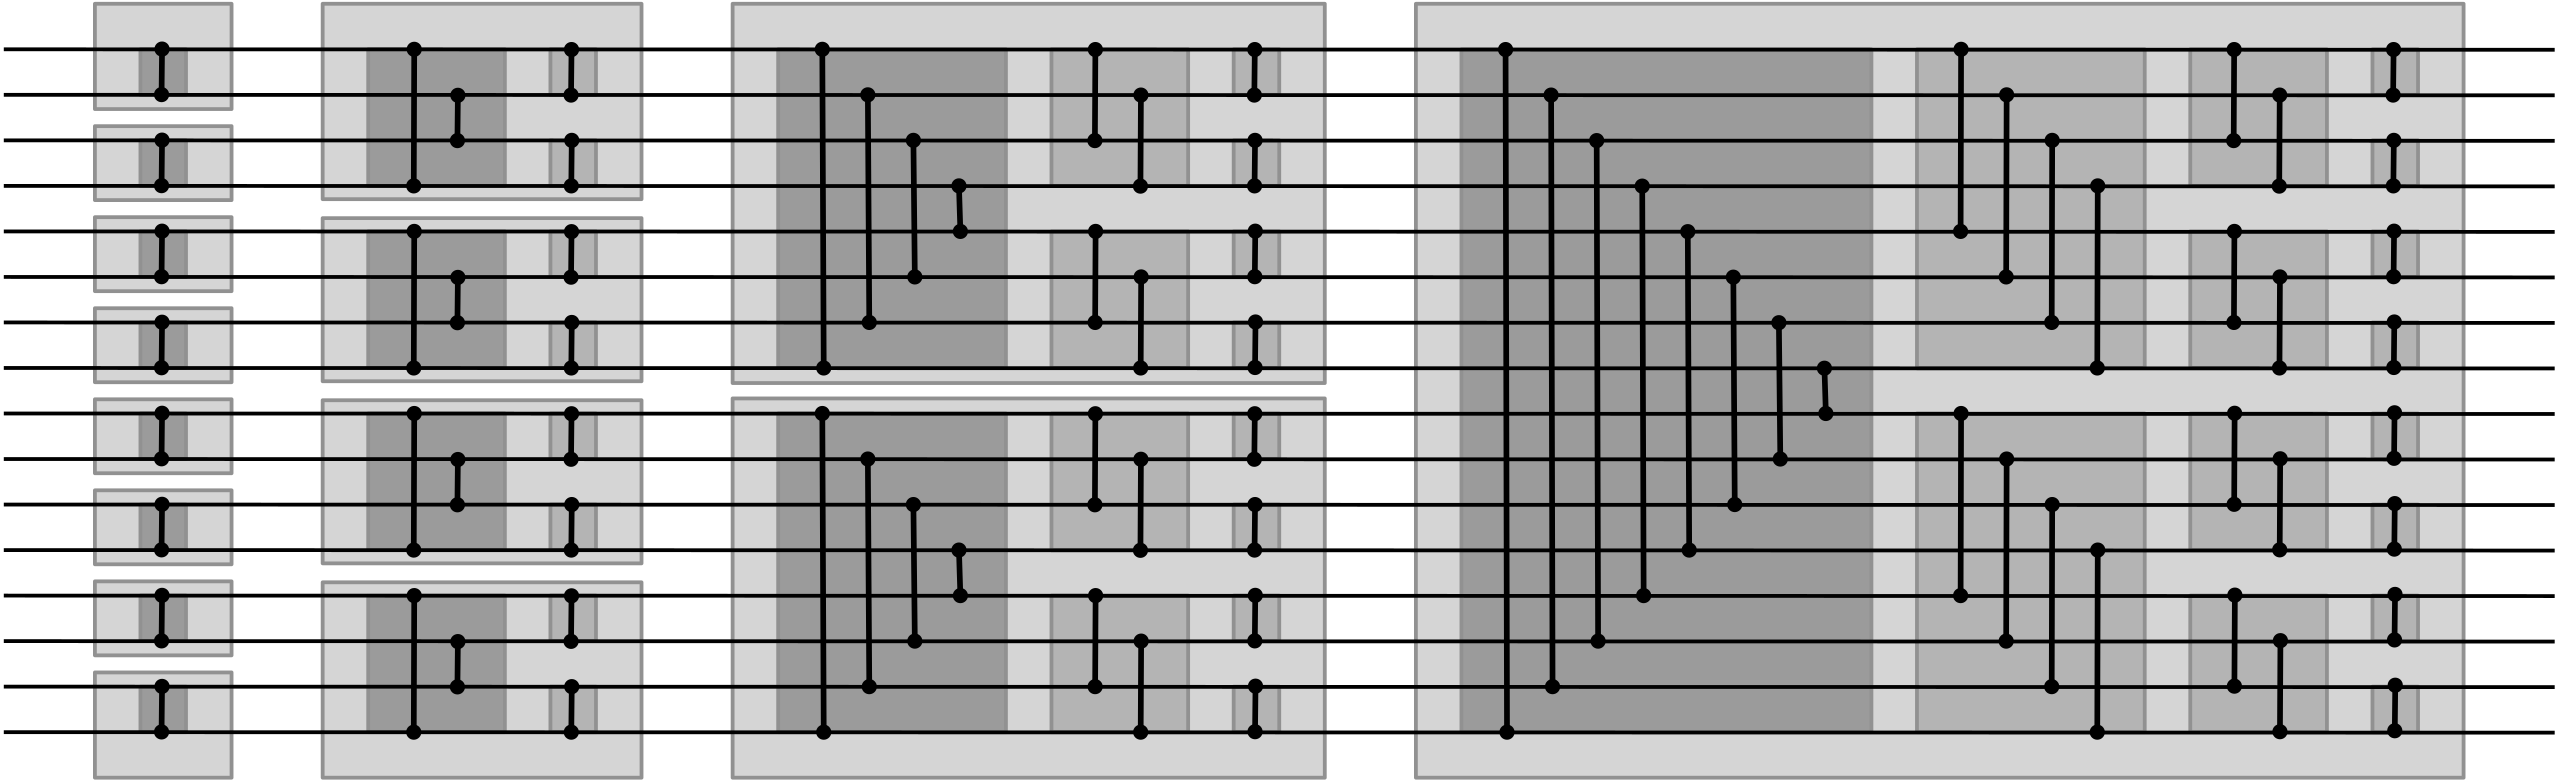
\includegraphics[width=\textwidth]{figures/bitonic-sort.png}
\caption{Sieć sortowania bitonicznego dla $N=16$: dziesięć przebiegów pogrupowanych
w cztery zewnętrzne etapy ($k=1,2,3,4$). Każdy wiersz odpowiada jednemu elementowi,
każda pionowa kreska --- komparatorowi obsługiwanemu przez osobny wątek GPU;
zagnieżdżone prostokąty zaznaczają granice kolejnych etapów zewnętrznych~\cite{christensen2021bitonic}}
\label{fig:bitonic_network}
\end{figure}

Implementacja na GPU mapuje każdy przebieg na osobne wywołanie potoku obliczeniowego.
Dwa parametry charakteryzujące dany przebieg --- wysokość aktualnego bloku bitonicznego
oraz bieżący krok wewnętrzny --- są przekazywane jako stałe wbudowane
(ang.~\textit{push constants}) bezpośrednio przed wywołaniem shadera; dzięki temu ten sam
skompilowany moduł obsługuje wszystkie sześć przebiegów bez konieczności tworzenia oddzielnych
potoków. Rozmiar grupy roboczej wynosi 256 wątków, a jedno wywołanie shadera pokrywa $256 \cdot 2 = 512$
sortowanych elementów, co dla $N$ cząstek przekłada się na $\lceil N/512 \rceil$ grup
roboczych na przebieg.

Zerowa rozbieżność wątków w połączeniu z prostotą operacji porównaj-i-zamień sprawia,
że sortowanie bitoniczne osiąga wysoką przepustowość dla zbiorów o rozmiarze rzędu
kilkudziesięciu tysięcy elementów --- skali typowej dla symulacji małej i średniej liczby
cząstek. Złożoność $O(N \log^2 N)$ staje się jednak coraz mniej korzystna w miarę wzrostu
$N$, co skłoniło do zbadania alternatywy opartej na zliczaniu, omówionej w kolejnym
podrozdziale.

\subsection{Radix Sort}
\label{subsec:radix}

Radix sort jest algorytmem sortowania przez zliczanie, a nie przez porównywanie, co stanowi
fundamentalną różnicę w stosunku do sortowania bitonicznego. Zamiast parować elementy,
każdy przebieg algorytmu zlicza, ile razy w danych pojawia się każda z $2^b$ możliwych
wartości wybranego $b$-bitowego fragmentu klucza, i na tej podstawie oblicza adresy docelowe
każdego elementu. Przy sortowaniu 32-bitowych kluczy po $b=8$ bitów na raz
($r = 2^8 = 256$ kubełków) potrzebne są dokładnie cztery przebiegi, co daje złożoność
$O(kN)$ przy stałym $k=4$ niezależnym od $N$ --- w praktyce liniowy wzrost kosztu z liczbą
sortowanych elementów~\cite{harada2011introduction}.

Każdy z czterech przebiegów rozkłada się na trzy kolejne shadery obliczeniowe
uruchamiane sekwencyjnie z barierami pamięci GPU między nimi: \textit{zliczanie},
\textit{skan prefiksowy} i \textit{reorganizacja}. Przepływ danych w jednym przebiegu
ilustruje rysunek~\ref{fig:radix_one_pass}.

\begin{figure}[h]
\centering
\begin{tikzpicture}[
  sbox/.style={draw, fill=green!10, rounded corners=3pt,
               minimum width=1.0cm, minimum height=1.2cm,
               font=\scriptsize, align=center},
  kbox/.style={draw, fill=blue!10, rounded corners=3pt,
               minimum width=2.8cm, minimum height=1.2cm,
               font=\scriptsize, align=center},
  dbox/.style={draw, fill=orange!10, rounded corners=3pt,
               minimum width=2.0cm, minimum height=1.2cm,
               font=\scriptsize, align=center},
  arr/.style={->, thick, >=Stealth}
]
  \node[sbox] (inp)  at ( 0.0,  0) {wej-\\[1pt]ście\\$N$ el.};
  \node[kbox] (cnt)  at ( 2.8,  0) {\textbf{zliczanie}\\dispatch $[m,1,1]$\\pam.\ dzielona};
  \node[dbox] (cbuf) at ( 5.9,  0) {liczniki\\$m \times 256$\\kol.-major};
  \node[kbox] (scn)  at ( 8.9,  0) {\textbf{skan}\\dispatch $[1,1,1]$\\Hillis--Steele};
  \node[dbox] (obuf) at (11.9,  0) {przesunięcia\\$m \times 256$\\in-place};
  \node[kbox] (ror)  at ( 8.9, -2.6) {\textbf{reorganizacja}\\dispatch $[m,1,1]$\\scatter};
  \node[sbox] (out)  at ( 5.9, -2.6) {wyj-\\[1pt]ście\\$N$ el.};

  \draw[arr] (inp)  -- (cnt);
  \draw[arr] (cnt)  -- (cbuf);
  \draw[arr] (cbuf) -- (scn);
  \draw[arr] (scn)  -- (obuf);
  \draw[arr] (obuf.south) |- (ror.east);
  \draw[arr] (ror)  -- (out);
\end{tikzpicture}
\caption{Przepływ danych w jednym przebiegu sortowania radix. Shadery zliczania
i reorganizacji uruchamiane są z $m = \lceil N/2048\rceil$ grupami roboczymi;
skan prefiksowy zawsze w pojedynczej grupie roboczej (dispatch $[1,1,1]$)
\newline Źródło: Opracowanie własne na podstawie~\cite{harada2011introduction}}
\label{fig:radix_one_pass}
\end{figure}

Shader \textit{zliczanie} jest wywoływany z $m = \lceil N/2048 \rceil$ grupami roboczymi,
gdzie każda przetwarza dokładnie $256 \times 8 = 2048$ elementów --- wynik przyjętego
rozmiaru grupy roboczej wynoszącego 256 wątków przy ośmiu elementach na wątek (stała
\texttt{ELEMENTS\_PER\_INVOCATION}). Każdy wątek wyodrębnia $b$-bitową cyfrę radix z
każdego ze swoich ośmiu elementów przez przesunięcie bitowe i maskowanie, a następnie
zlicza jej wystąpienia operacją atomową \texttt{atomicAdd} na tablicy
\texttt{local\_counts[256]} przechowywanej w pamięci dzielonej grupy roboczej. Koszt
operacji atomowej na pamięci dzielonej jest wielokrotnie niższy niż na pamięci globalnej
GPU --- bez tego kroku wszystkie wątki wszystkich grup roboczych konkurowałyby o te same
256 globalnych liczników, co skutkowałoby serializacją i niwelowałoby zyski z równoległości.
Po przetworzeniu całego segmentu bariera synchronizuje lokalne liczniki w obrębie grupy,
a jeden wątek zapisuje 256 wartości do globalnego bufora liczników pod indeksem
$d \cdot m + \mathrm{wg}$, gdzie $d$ to wartość cyfry radix, a $\mathrm{wg}$ --- numer
grupy roboczej. Ten kolumnowy układ bufora jest nieprzypadkowy: podczas skanowania
kolejne wątki odczytują wartości tego samego kubełka $d$ z kolejnych segmentów pod
kolejnymi adresami pamięci, co zapewnia koalescencję dostępów do pamięci globalnej.

Shader \textit{skan prefiksowy} wywoływany jest zawsze jako pojedyncza grupa robocza
o rozmiarze 256 wątków (dispatch $[1,1,1]$), niezależnie od liczności $N$. Jedna grupa
przekształca tablicę $m \times 256$ liczników w tablicę globalnych przesunięć metodą
Hillisa--Steele'a~\cite{harada2011introduction} w trzech fazach: najpierw obliczana jest
wyłączna suma prefiksowa w obrębie każdego wiersza tablicy, dając lokalne przesunięcia
wewnątrz grupy roboczej; następnie przeprowadzana jest włączna suma prefiksowa po
sumarycznych zliczeniach każdego kubełka; na końcu globalne przesunięcia bloków są
dodawane z powrotem, kompletując tablicę adresów docelowych. Wybór pojedynczej grupy
roboczej eliminuje konieczność wielopoziomowej synchronizacji globalnej, która byłaby
niezbędna przy wielogrupowym skanowaniu --- jest to możliwe właśnie dlatego, że liczba
kubełków wynosi 256, co odpowiada typowej szerokości SIMD architektury GPU i mieści się
w jednej grupie roboczej.

Shader \textit{reorganizacja} przywraca pełny paralelizm: wywoływany z $m$ grupami
roboczymi przetwarzającymi po 2048 elementów każda. Dla każdego elementu wątek oblicza
adres docelowy jako sumę globalnego przesunięcia odczytanego z tablicy przesunięć oraz
lokalnego indeksu tego elementu w obrębie grupy roboczej i kubełka, po czym zapisuje
go pod ten adres w buforze wyjściowym. Operacja ta jest stabilnym scatterem ---
zachowuje wzajemną kolejność elementów o tej samej wartości cyfry radix, co jest
warunkiem koniecznym poprawności całego algorytmu: przebiegi od najmniej znaczących
bitów (ang.~\textit{LSB first}) ku najbardziej znaczącym zachowują poprawną kolejność
z poprzednich przebiegów wyłącznie wtedy, gdy każdy bieżący przebieg jest stabilny.

Implementacja korzysta z dwóch buforów sortowania: głównego \texttt{grid\_entries}
oraz pomocniczego \texttt{entries\_tmp}, wewnętrznego do struktury \texttt{RadixSorter}.
Parzyste przebiegi (0 i~2) kierują dane z \texttt{grid\_entries} do \texttt{entries\_tmp},
nieparzyste (1 i~3) --- w odwrotnym kierunku; po czterech przebiegach wynik jest zawsze
z powrotem w \texttt{grid\_entries}. Złożoność $O(kN)$ ze stałym $k=4$
sprawia, że koszt sortowania rośnie liniowo z liczbą cząstek, co czyni radix sort
algorytmem z wyboru dla dużych symulacji, gdzie logarytmiczne czynniki sortowania
bitonicznego stają się odczuwalne.

\subsection{Porównanie algorytmów}
\label{subsec:sort_comparison}

Mając zaimplementowane oba algorytmy sortowania, można je porównać
zarówno pod kątem właściwości strukturalnych, jak i rzeczywistej wydajności
na GPU. Tabela~\ref{tab:sort_comparison} zestawia najważniejsze cechy obu
metod, podkreślając te różnice, które bezpośrednio wpływają na koszt
wykonania w potoku obliczeniowym.

\begin{table}[htbp]
\centering
\caption{Porównanie własności sortowania bitonicznego i radix}
\label{tab:sort_comparison}
\begin{tabular}{p{4.5cm}p{4.5cm}p{4.5cm}}
\toprule
\textbf{Cecha} & \textbf{Bitonic sort} & \textbf{Radix sort} \\
\midrule
Złożoność czasowa & $O(N \log^2 N)$ & $O(kN)$, $k=4$ \\[3pt]
Liczba dispatchów dla $N=2^{15}$ & 120 & 12 \\[3pt]
Rozbieżność wątków & Zerowa & Zerowa \\[3pt]
Pamięć pomocnicza & Brak (sort. w miejscu) & Bufor \texttt{entries\_tmp} ($8N$~B) i bufor liczników \\[3pt]
Stabilność sortowania & Niestabilna & Stabilna \\[3pt]
Wymóg na $N$ & Potęga dwójki & Dowolne \\
\bottomrule
\end{tabular}
\end{table}

Bezpośredni pomiar czasu sortowania w funkcji liczby elementów $N$
przeprowadzono w środowisku testowym opartym na bezokienkowym kontekście
Vulkan, z buforem wypełnianym pseudolosowymi kluczami
przed każdym uruchomieniem. Czas dla każdego punktu pomiaru wyznaczono jako
medianę z piętnastu niezależnych przebiegów, poprzedzonych trzema przebiegami
rozgrzewkowymi pokrywającymi koszt kompilacji shaderów przez sterownik.
Wyniki, dla $N$ rosnącego od $2^{10}$ do $2^{22}$, przedstawia
rysunek~\ref{fig:sort_benchmark}.

\begin{figure}[H]
\centering
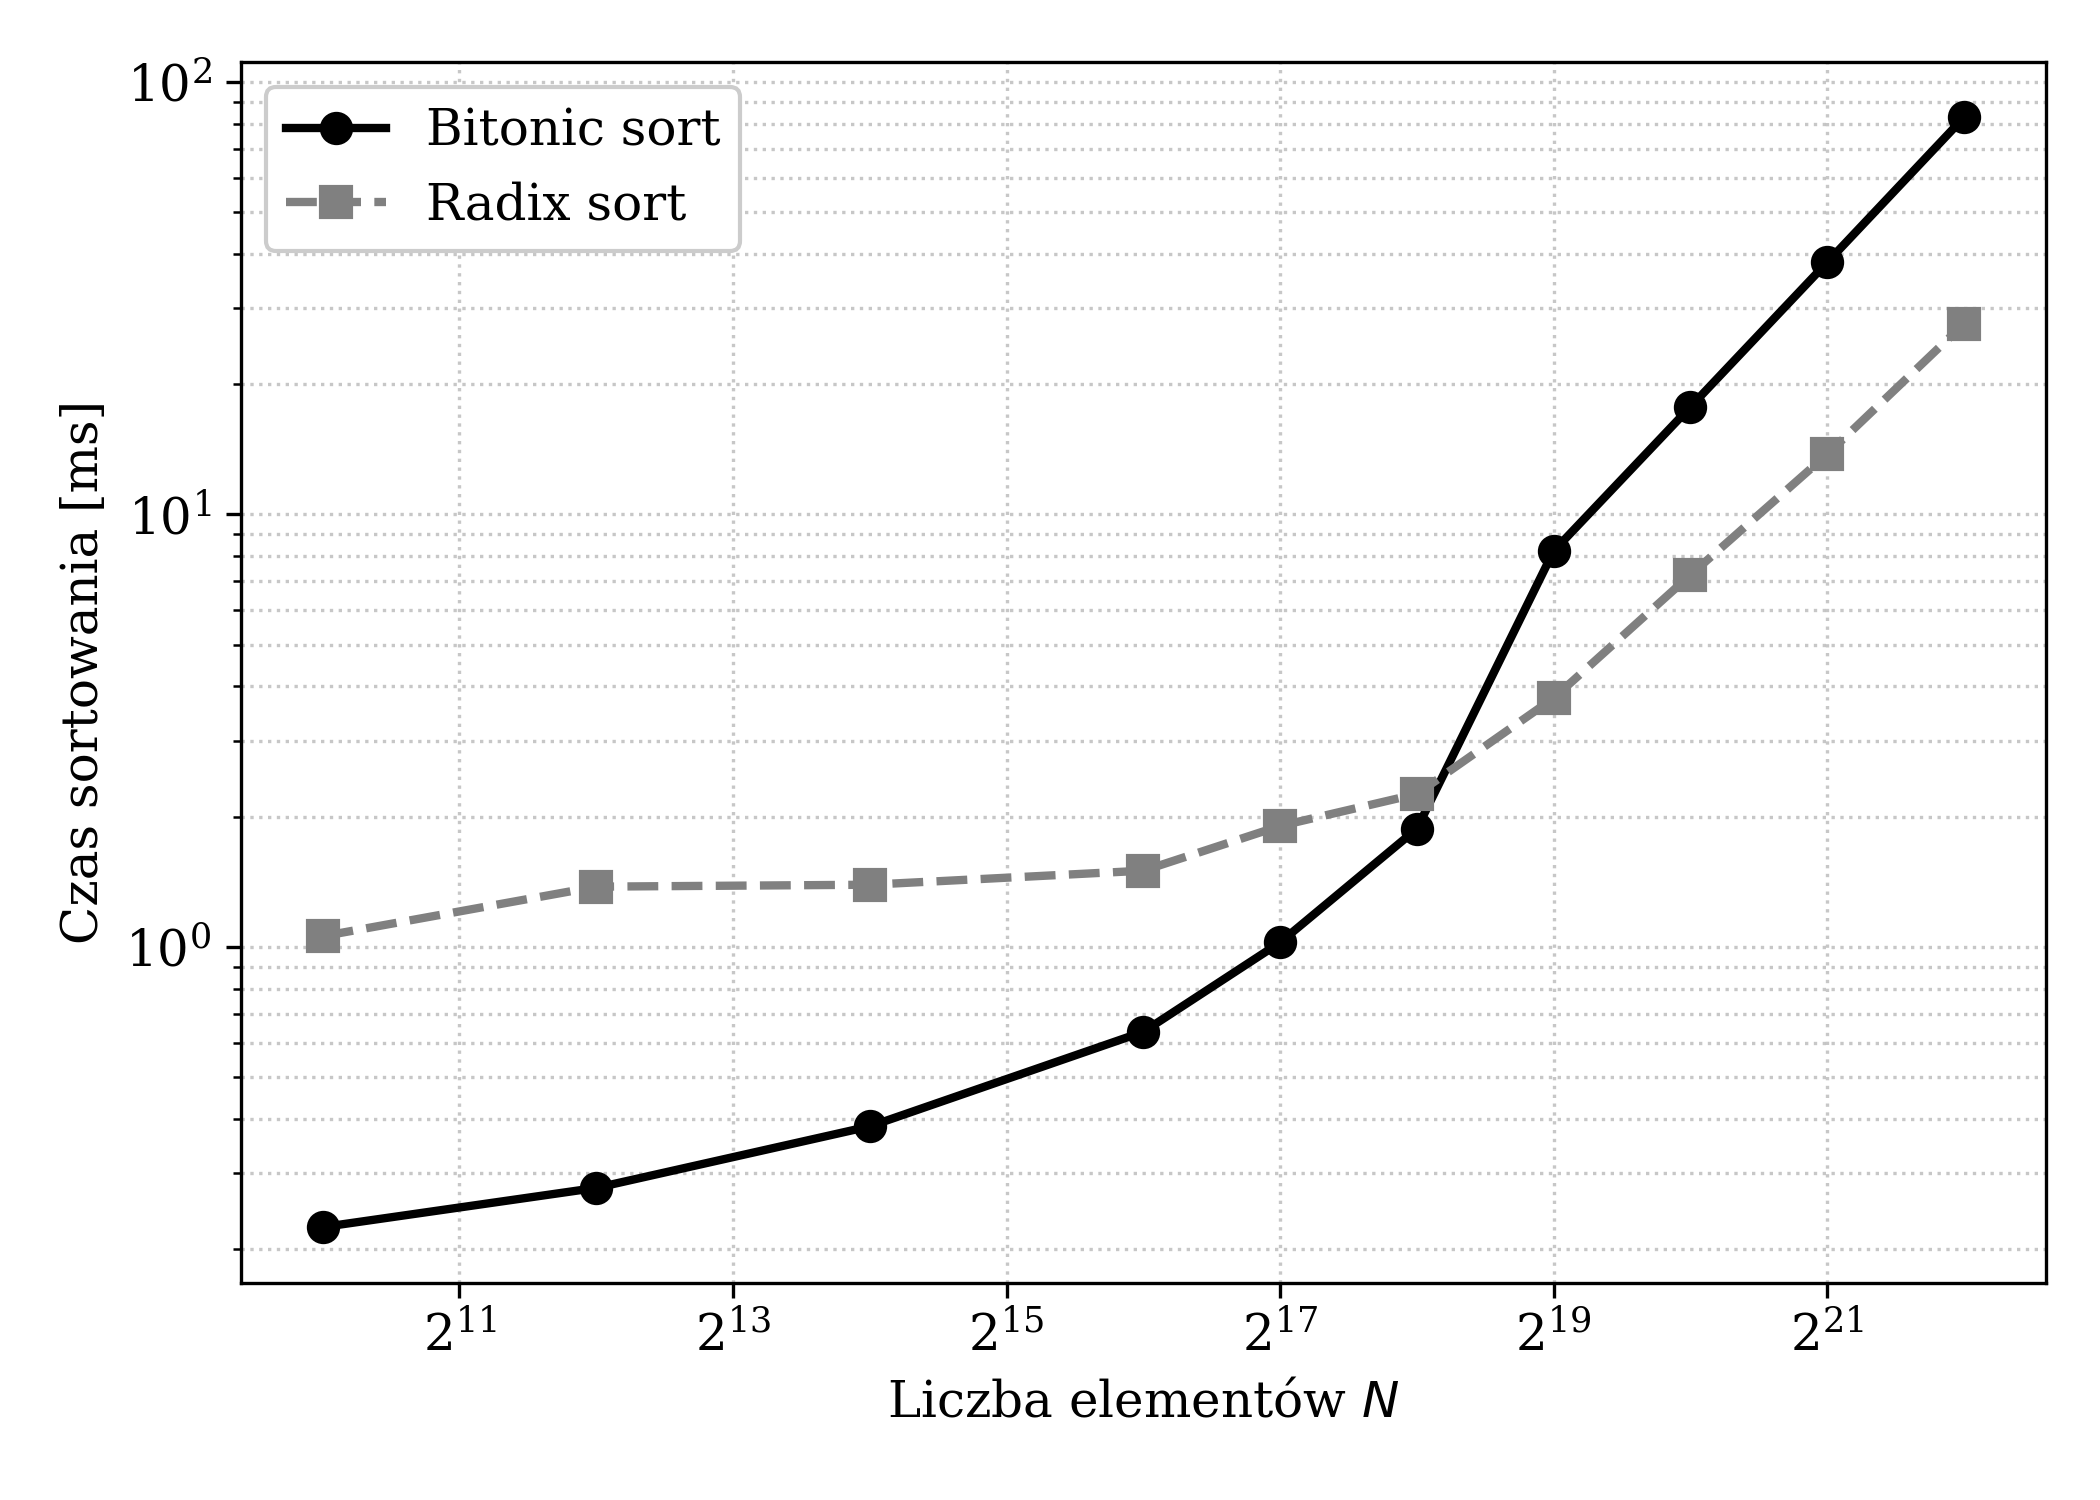
\includegraphics[width=0.85\textwidth]{figures/sort_benchmark.png}
\caption{Czas sortowania bufora \texttt{grid\_entries} jako funkcja liczby
elementów $N$, w skali logarytmicznej na obu osiach. Punkty odpowiadają
medianie z piętnastu przebiegów dla danego $N$
\newline Źródło: Opracowanie własne}
\label{fig:sort_benchmark}
\end{figure}

Dla małej liczby elementów ($N \lesssim 2^{18}$) sortowanie bitoniczne jest
szybsze mimo asymptotycznie gorszej złożoności. Wynika to z bardzo niskiego
stałego narzutu pojedynczego komparatora: każdy przebieg bitoniczny składa się
wyłącznie z odczytu pary elementów, porównania i warunkowej zamiany, podczas
gdy każdy przebieg radix wymaga trzech kolejnych dispatchów ze wzajemną
synchronizacją barierami pamięci. Przy $N \le 2^{14}$ cała praca obliczeniowa
sortowania mieści się w czasie porównywalnym z kosztem wprowadzenia poleceń
do kolejki GPU --- pomiar jest zdominowany przez ten stały narzut, a różnica
między algorytmami pochodzi głównie z liczby dispatchów składowych.

Punkt równowagi obserwuje się między $N = 2^{18}$ a $N = 2^{19}$. Powyżej tego
progu logarytmiczny czynnik bitonicznego $O(N \log^2 N)$ zaczyna dominować nad
stałą liczbą dwunastu dispatchów radix. Dla $N = 2^{22}$ (ponad cztery miliony
elementów) sortowanie radix jest niemal trzykrotnie szybsze: $30{,}5$~ms
względem $82{,}6$~ms dla bitonicznego.

Pomiar wyizolowanego sortowania nie odzwierciedla jednak w pełni zachowania
algorytmu w pełnym potoku obliczeniowym, w którym dispatche sortowania są
przeplatane innymi etapami solvera DFSPH wraz z wymaganymi między nimi
barierami pamięci. Profil Tracy zarejestrowany dla symulacji z 25\,000 cząstek
(rysunki~\ref{fig:tracy_bitonic} i~\ref{fig:tracy_radix}) pokazuje, że średni
czas wykonania etapu \texttt{neighbor\_search\_post\_integrate} ---
obejmującego haszowanie, sortowanie, wyznaczenie przesunięć i reorganizację
buforów --- wynosi $3{,}64$~ms dla wariantu bitonicznego i $616{,}3$~µs
dla wariantu radix. Oba pomiary dotyczą tej samej konfiguracji symulacji,
więc niemal sześciokrotna różnica wynika wyłącznie z wyboru algorytmu
sortowania.

\begin{figure}[htbp]
\centering
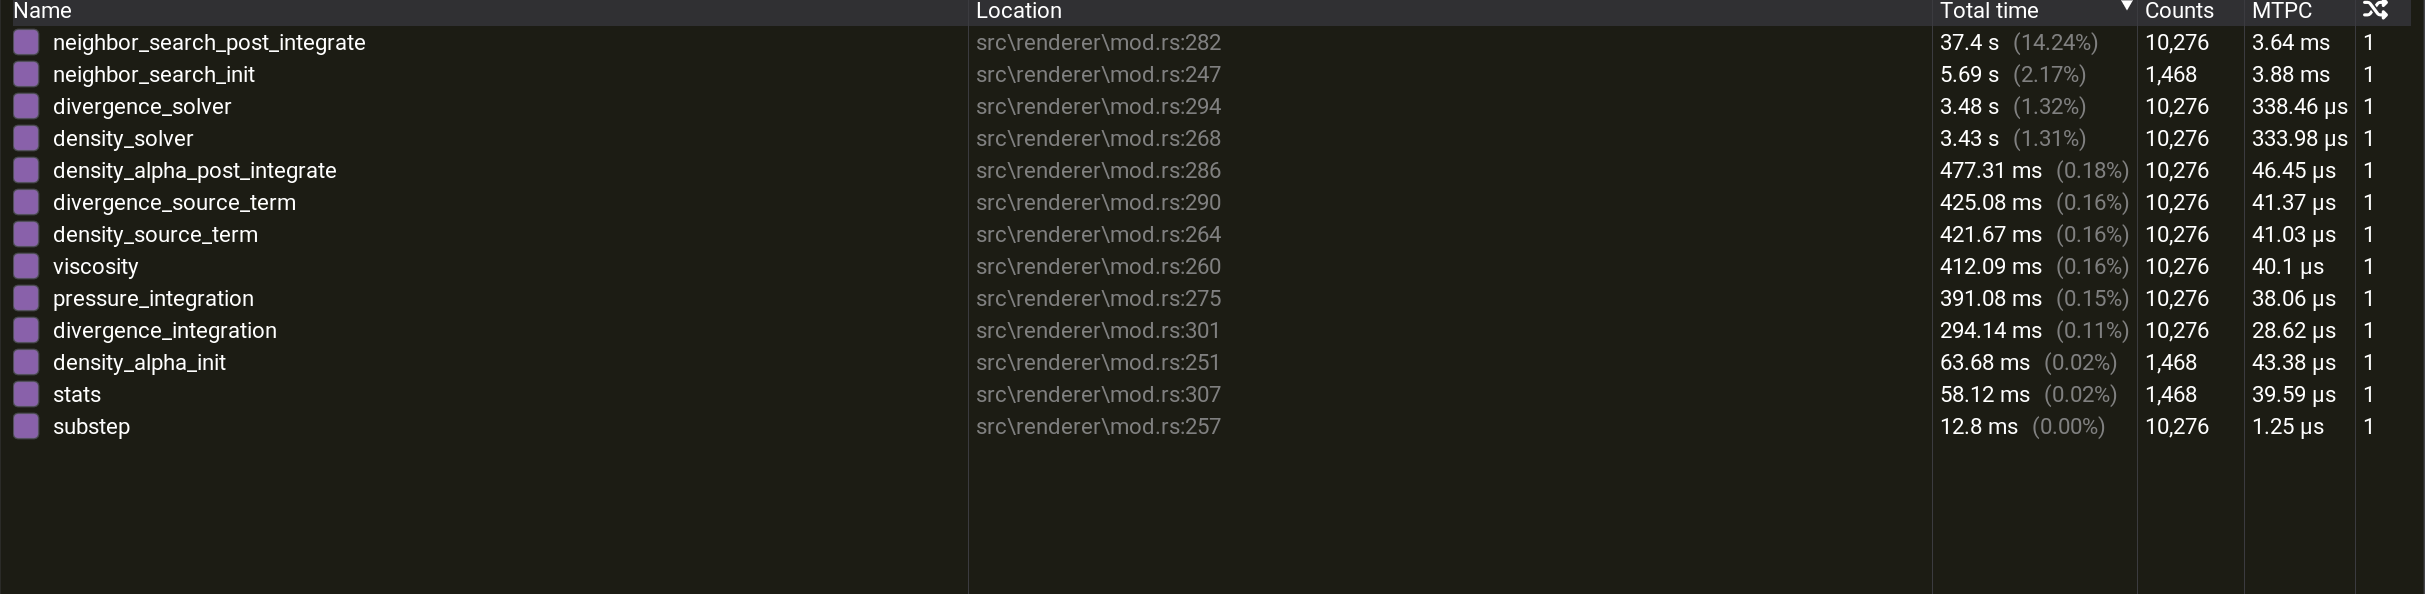
\includegraphics[width=0.95\textwidth]{figures/bitonic_tracy_profile.png}
\caption{Profil Tracy dla wariantu z sortowaniem bitonicznym, $N=25\,000$
cząstek. Wiersz \texttt{neighbor\_search\_post\_integrate} pokazuje średni
czas $3{,}64$~ms na wywołanie
\newline Źródło: Opracowanie własne}
\label{fig:tracy_bitonic}
\end{figure}

\begin{figure}[htbp]
\centering
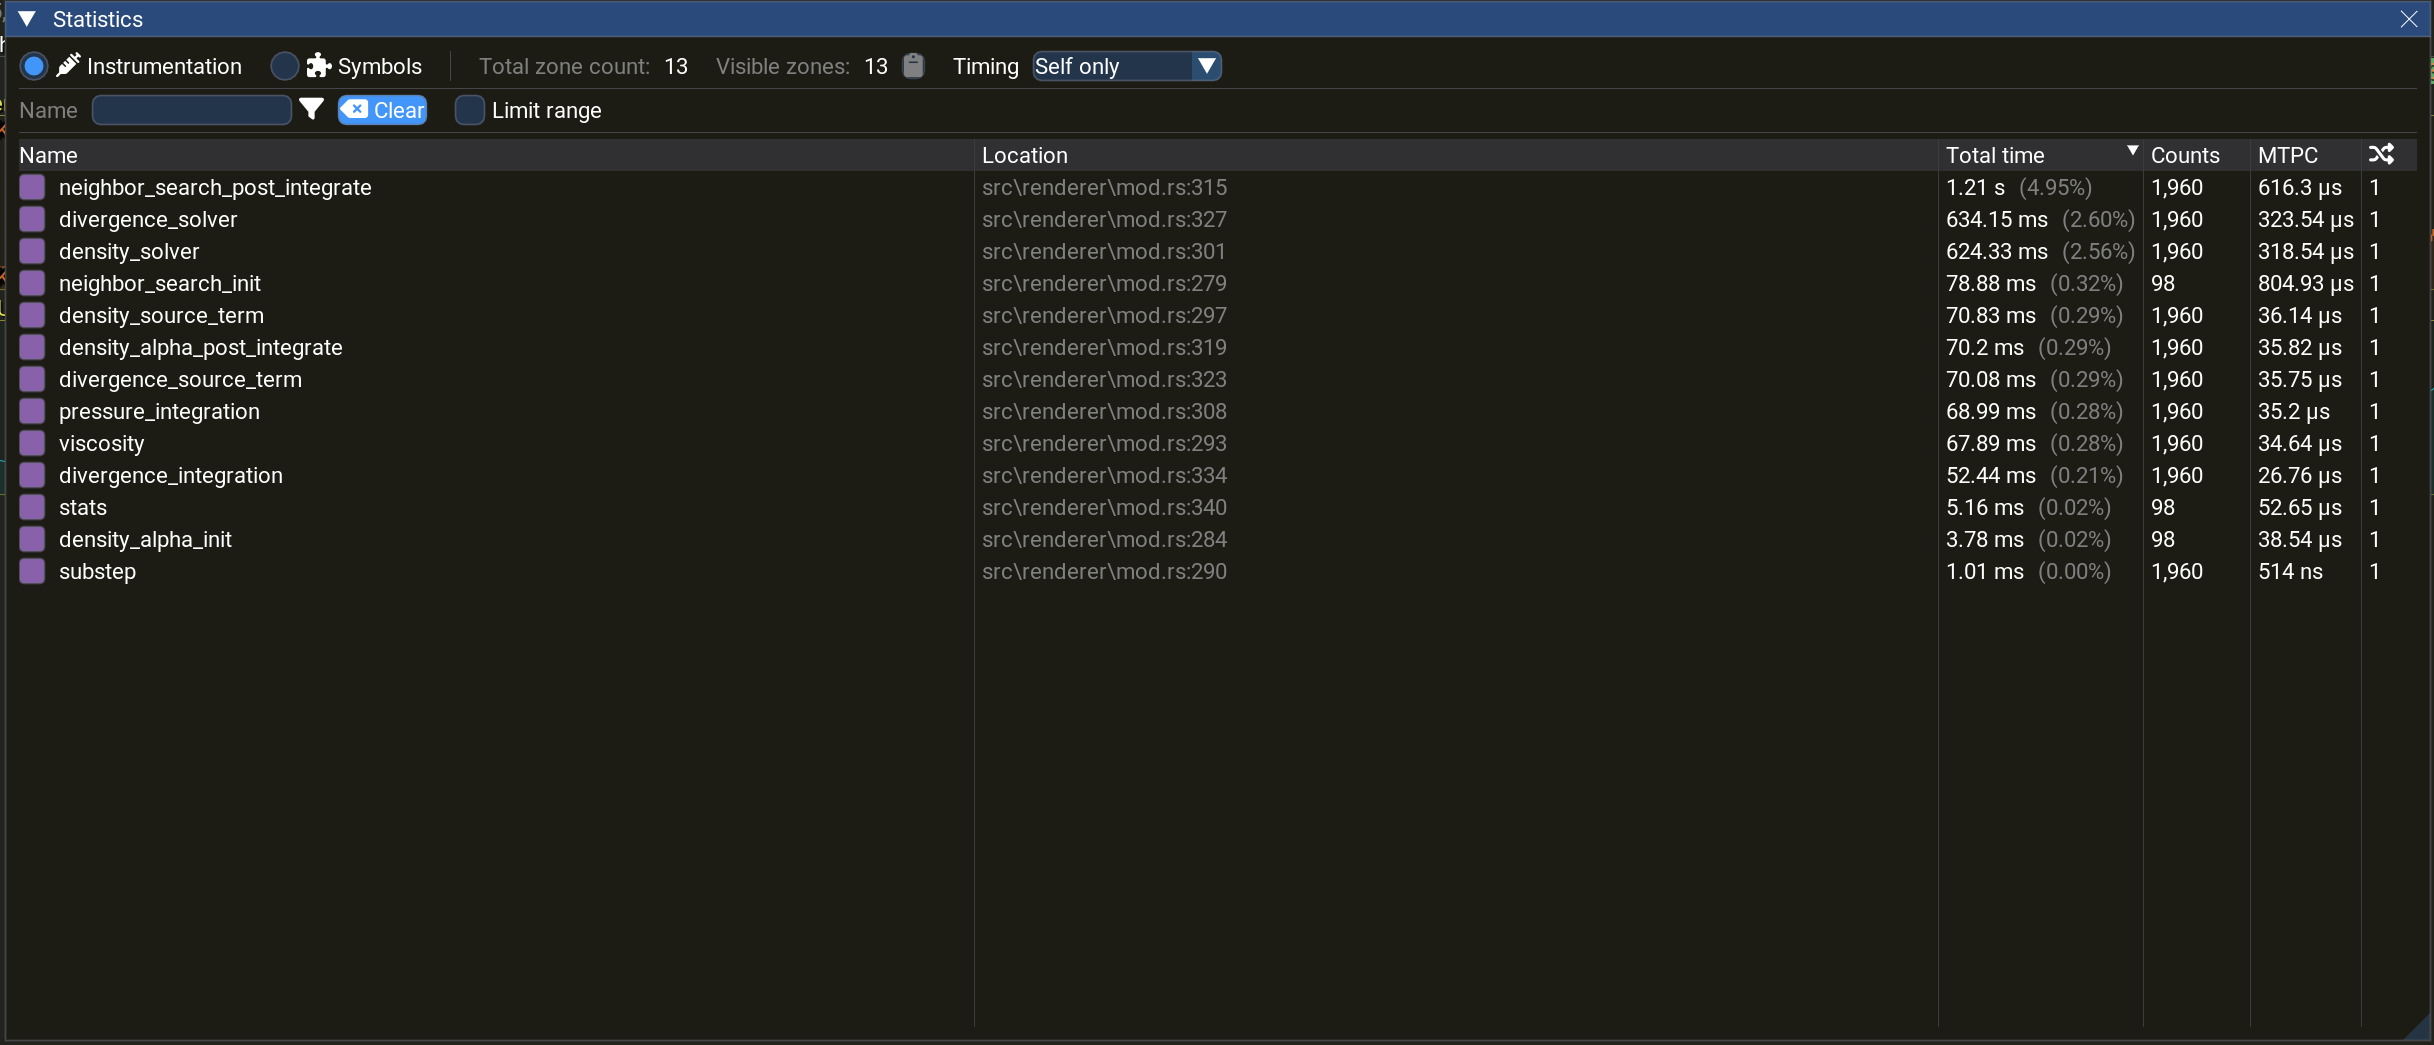
\includegraphics[width=0.95\textwidth]{figures/radix_tracy_profile.png}
\caption{Profil Tracy dla wariantu z sortowaniem radix w tym samym
scenariuszu. Średni czas tego samego zakresu spada do $616{,}3$~µs
\newline Źródło: Opracowanie własne}
\label{fig:tracy_radix}
\end{figure}

Rozbieżność między izolowanym testem porównawczym (gdzie radix dla $N = 2^{15}$ jest
nieznacznie wolniejszy) a pomiarem produkcyjnym (gdzie ten sam $N$ daje
sześciokrotne przyspieszenie) ma uzasadnienie strukturalne. Sortowanie
bitoniczne $32\,768$ elementów ($\lceil 25\,000 \rceil_2$) wymaga
$\frac{\log_2^2 32768 + \log_2 32768}{2} = 120$ dispatchów, z których każdy
w pełnym potoku jest oddzielony od kolejnego barierą pamięci wstawioną przez
\texttt{AutoCommandBufferBuilder}; radix wymaga ich jedynie dwunastu. W teście
izolowanym, gdzie GPU wykonuje wyłącznie sortowanie, koszt pojedynczej bariery
jest amortyzowany przez wysoką zajętość jednostek obliczeniowych. W pełnym
potoku DFSPH bariera staje się jawnym punktem synchronizacji, ponieważ
poprzedza ją zapis innego shadera obliczeniowego --- a sumaryczny koszt skaluje
się z liczbą dispatchów algorytmu sortowania.

Łączny obraz prowadzi do jednoznacznego wyboru: dla każdego rozmiaru symulacji
od kilku tysięcy cząstek wzwyż radix sort jest szybszym wariantem, a jego
przewaga rośnie zarówno z $N$, jak i z liczbą innych etapów obliczeniowych
dzielących GPU. Sortowanie bitoniczne pozostaje w kodzie jako alternatywa
dostępna do przełączenia w czasie wykonania przez wariant
\texttt{SortAlgorithm::Bitonic}, użyteczna w celach porównawczych oraz
w scenariuszach, w których prostota sieci komparatorów ma znaczenie większe
niż mierzona wydajność.

% ------------------------------------------------------------
\section{Solver DFSPH}
\label{sec:dfsph}

Wszystkie wcześniejsze sekcje tej części pracy --- organizacja pamięci
w układzie SOA z parami buforów dla pozycji i prędkości, haszowanie
przestrzenne wraz z sortowaniem i reorganizacją buforów oraz autorska
cecha \texttt{ComputeStep} unifikująca cykl życia potoków obliczeniowych
--- istnieją wyłącznie po to, by w tym miejscu mogła zostać zrealizowana
sama symulacja dynamiki cieczy. Dyskretyzacja jądrowa metody SPH
wprowadzona w podrozdziale~\ref{subsec:kernel-interpolation},
dwuetapowa korekcja DFSPH zdefiniowana algorytmami~\ref{alg:density_source}
i~\ref{alg:div_source} oraz konkretne struktury danych z sekcji~\ref{sec:data_structures}
zbiegają się tutaj w jeden spójny potok obliczeniowy. Każdy z jego etapów
jest osobnym implementatorem cechy \texttt{ComputeStep} i odpowiada
konkretnemu fragmentowi matematycznego sformułowania metody; ich kolejność
oraz wzajemne zależności określają, w jaki sposób abstrakcyjne równania
teoretyczne odwzorowują się na rzeczywiste shadery obliczeniowe wykonywane
na GPU.

Z implementacyjnego punktu widzenia kluczowa jest asymetria między obydwoma
poziomami korekcji: \textit{korekcja gęstości} kończy się adwekcją pozycji
$\mathbf{p}_i \leftarrow \mathbf{p}_i + \Delta t\,\mathbf{v}_i$,
natomiast \textit{korekcja dywergencji} działa wyłącznie na buforze
prędkości i nie modyfikuje pozycji cząstek.
Ta różnica determinuje kolejność shaderów w pętli substepów.
Poza nią oba poziomy współdzielą identyczną strukturę: iteracyjna pętla
ciśnienia z tym samym wzorcem dostępu do sąsiedztwa, różniąca się
wyłącznie wyrazem źródłowym i finalnym krokiem integracji.

Wszystkie shadery realizujące fizykę SPH dzielą jeden fundamentalny wzorzec
dostępu do danych. Niezależnie od tego, czy obliczają gęstość, wyraz
źródłowy, siłę ciśnienia czy korekcję lepkościową, każdy z nich akumuluje
sumę po geometrycznym sąsiedztwie cząstki~$i$, ważoną jądrem~$W$ lub jego
gradientem~$\nabla W$. Konkretna postać akumulowanej wielkości różni się
między etapami, lecz struktura pętli pozostaje niezmiennikiem całego potoku.
Wykorzystując bufor \texttt{grid\_start} przygotowany przez potok
wyszukiwania sąsiadów (sekcja~\ref{sec:neighbor_search}), każdy shader
wyznacza komórkę przestrzenną swojej cząstki i iteruje po
$3 \times 3 \times 3 = 27$ komórkach sąsiednich, używając ich skrótów jako
indeksów wejścia do listy posortowanych wpisów.
Jądro $W(\|\mathbf{r}\|, h)$ zwraca skalarną wagę, malejącą z odległością;
jego gradient $\nabla W(\mathbf{r}, h)$ jest wektorem wskazującym kierunek
i tempo zmian tej wagi.
W obliczeniach SPH $W$ pojawia się wszędzie tam, gdzie sumujemy wielkości
skalarne --- jak gęstość --- natomiast $\nabla W$ wszędzie tam, gdzie
potrzebna jest siła lub przyspieszenie.
Algorytm~\ref{alg:neighbor_iter} przedstawia ten uniwersalny wzorzec.

\begin{algorithm}[htbp]
\caption{Wspólny wzorzec iteracji po sąsiadach w shaderach SPH}
\label{alg:neighbor_iter}
$\mathbf{c}_i \leftarrow \lfloor \mathbf{p}_i / h \rfloor$\;
\For{$dz \in \{-1,\,0,\,+1\}$}{
  \For{$dy \in \{-1,\,0,\,+1\}$}{
    \For{$dx \in \{-1,\,0,\,+1\}$}{
      $k \leftarrow \mathrm{hash}(\mathbf{c}_i + (dx, dy, dz))$\;
      $s \leftarrow \texttt{grid\_start}[k]$\;
      \While{$s < M$ \upshape \textnormal{i} $\texttt{grid\_entries}[s].\texttt{hash} = k$}{
        $j \leftarrow \texttt{grid\_entries}[s].\texttt{index}$\;
        $\mathbf{r}_{ij} \leftarrow \mathbf{p}_i - \mathbf{p}_j$\;
        \If{$\|\mathbf{r}_{ij}\| < h$}{
          akumulacja wkładu pary $(i, j)$ z wagą $W(\|\mathbf{r}_{ij}\|,\,h)$ lub $\nabla W(\mathbf{r}_{ij},\,h)$\;
        }
        $s \leftarrow s + 1$\;
      }
    }
  }
}
\end{algorithm}

Identyczna pętla iteracji po sąsiadach występuje we wszystkich shaderach solvera DFSPH
--- różni je wyłącznie wyrażenie pod sumą
oraz atrybut, do którego trafia wynik akumulacji. Dzięki przepisaniu pozycji
i prędkości na bufory \texttt{\_b} przez etap \texttt{reorder}
(\ref{subsec:neighbor_pipeline}), kolejne wpisy danej komórki leżą gęsto
w pamięci, a odczyt całego 27-elementowego sąsiedztwa wykonuje się
w niewielkiej liczbie skoalescowanych transakcji pamięci globalnej GPU.

Tabela~\ref{tab:dfsph_variable_mapping} odwzorowuje wielkości figurujące
w sformułowaniu matematycznym DFSPH na konkretne bufory struktury
\texttt{GpuPhysicsData} oraz na shadery odpowiedzialne za ich zapis.
Ze względu na podwójne buforowanie cząstek (\ref{subsec:gpu_buffers}),
pozycje i prędkości występują w dwóch wariantach: bufor \texttt{\_a}
przechowuje stabilny stan wejściowy, na podstawie którego haszowanie
przestrzenne wyznacza komórki cząstek; bufor \texttt{\_b}, do którego
\texttt{reorder} przepisuje dane w kolejności sprzyjającej lokalności
odczytu, stanowi wejście dla wszystkich kolejnych etapów solvera.
Pozostałe wielkości to jednowymiarowe tablice indeksowane numerem cząstki.

\begin{table}[H]
\centering
\caption{Odwzorowanie wielkości teoretycznych DFSPH na bufory GPU}
\label{tab:dfsph_variable_mapping}
\begin{tabular}{p{4.8cm}p{4.5cm}p{4.5cm}}
\toprule
\textbf{Wielkość} & \textbf{Bufor} & \textbf{Etap zapisujący} \\
\midrule
$\mathbf{p}_i$ --- pozycja                  & \texttt{position\_a}, \texttt{position\_b}    & \texttt{reorder}, \texttt{pressure\_integration} \\[3pt]
$\mathbf{v}_i$ --- prędkość                 & \texttt{velocity\_a}, \texttt{velocity\_b}    & \texttt{reorder}, \texttt{viscosity}, korekcje ciśnienia \\[3pt]
$\rho_i$ --- gęstość                        & \texttt{densities}                            & \texttt{density\_alpha} \\[3pt]
$\alpha_i$ --- współczynnik DFSPH           & \texttt{factors}                              & \texttt{density\_alpha} \\[3pt]
$s_i$ --- wyraz źródłowy                    & \texttt{source\_terms}                        & \texttt{density\_source\_term}, \texttt{divergence\_source\_term} \\[3pt]
$p_i$ --- ciśnienie                         & \texttt{pressures}                            & \texttt{pressure\_update} \\[3pt]
$\mathbf{a}_i^{p}$ --- przysp. ciśnienia    & \texttt{pressure\_accelerations}              & \texttt{pressure\_force} \\
\bottomrule
\end{tabular}
\end{table}

Pozostałe podrozdziały tej sekcji szczegółowo omawiają poszczególne
komponenty solvera. Podrozdział~\ref{subsec:substep_loop} przedstawia
pełną pętlę substepów ustalającą kolejność wszystkich etapów wewnątrz
pojedynczej klatki. Podrozdział~\ref{subsec:density} opisuje obliczanie
gęstości $\rho_i$ oraz współczynnika $\alpha_i$, pełniącego rolę
prekondycjonera w solverze ciśnienia.
Podrozdziały~\ref{subsec:density_correction}
i~\ref{subsec:divergence_correction} analizują kolejno korekcję gęstości
i korekcję dywergencji --- dwie iteracyjne pętle ciśnienia, które łącznie
wymuszają nieściśliwość pola prędkości. Podrozdział~\ref{subsec:cfl}
omawia warunek CFL i strategię doboru kroku czasowego $\Delta t$.

\subsection{Pętla substepów}
\label{subsec:substep_loop}

Pełna sekwencja wywołań shaderów w obrębie substepu ukazana jest
w Algorytmie~\ref{alg:frame_loop}.
Bezpośrednio po adwekcji następuje przebudowa struktury wyszukiwania
sąsiadów. To drugie wywołanie \texttt{neighbor\_search} w obrębie jednego
substepu nie jest redundancją --- jest koniecznością wynikającą z fizycznego
przemieszczenia cząstek.
Tablica \texttt{grid\_start}, zbudowana przed substepem, indeksuje pozycje
sprzed adwekcji; korekcja dywergencji oparta na nieaktualnej strukturze
obliczałaby gradient prędkości $\nabla \cdot \mathbf{v}$ względem błędnych
sąsiadów, co prowadziłoby do narastających błędów kompresji szczególnie
widocznych przy dużych prędkościach cząstek.
Po przebudowie sąsiedztwa i ponownym wyznaczeniu $\rho_i$, $\alpha_i$
faza dywergencji przebiega analogicznie: iteracyjna pętla $N_\nabla$ razy
uruchamia ten sam \texttt{pressure\_force} i \texttt{pressure\_update}
z wyrazem źródłowym opartym na dywergencji pola prędkości,
po czym \texttt{divergence\_integration} aktualizuje prędkości
bez modyfikowania pozycji.

Iteracyjny charakter obu solwerów wynika z natury problemu.
Zmiana ciśnienia cząstki~$i$ generuje przyspieszenie oddziałujące na
jej sąsiadów, które z kolei wymagają korekty swoich ciśnień ---
i tak dalej.
Jedno przejście pętli realizuje krok analogiczny do iteracji Jacobiego:
wyznacza lokalną poprawkę przy założeniu, że ciśnienia sąsiadów pozostają
chwilowo zamrożone.
Kilka takich kroków ($N_\rho = 2$--$5$, $N_\nabla = 1$--$3$)
zazwyczaj wystarcza do sprowadzenia średniego błędu poniżej zadanego progu;
strategię doboru tych liczb omówiono w podrozdziale~\ref{subsec:cfl}.

\subsection{Obliczanie gęstości}
\label{subsec:density}

Szader \texttt{density\_and\_alpha} oblicza w jednym przebiegu dwie
wielkości: gęstość $\rho_i$ oraz współczynnik $\alpha_i$~\cite{bender2015divergence}.
Listing~\ref{lst:density_alpha} przedstawia funkcję \texttt{main()} shadera.

\begin{lstlisting}[caption={Szader \texttt{density\_and\_alpha} --- logika akumulacji},
                   label=lst:density_alpha,]
void main() {
    uint i = gl_GlobalInvocationID.x;
    if (i >= uint(positions.length())) return;

    float density     = 0.0;
    float sum_grad_sq = 0.0;
    vec3  grad_sum    = vec3(0.0);

    // iteracja po 27 sąsiednich komórkach
    float r = sqrt(dot(r_vec, r_vec));
    density += mass * kernel_w(r, h);
    if (r > 1e-6) {
        vec3 mass_grad  = mass * kernel_grad(r_vec, r, h);
        grad_sum       += mass_grad;
        sum_grad_sq    += dot(mass_grad, mass_grad);
    }
    // koniec petli

    densities[i] = density;
    float alpha = sum_grad_sq + dot(grad_sum, grad_sum);
    if (alpha > 1e-6) { factors[i] = alpha; }
    else              { factors[i] = 0.0;   }
}
\end{lstlisting}

Każda invokacja odpowiada jednej cząstce~$i$.
Zmienna \texttt{density} akumuluje skalarne wkłady jądra \texttt{kernel\_w}
po 27 sąsiednich komórkach --- jest to bezpośrednia realizacja wzorca
z Algorytmu~\ref{alg:neighbor_iter}.
Zmienne \texttt{grad\_sum} i \texttt{sum\_grad\_sq} akumulują jednocześnie
składniki współczynnika $\alpha_i$: odpowiednio sumę gradientów
$\sum_j m\nabla W_{ij}$ oraz sumę ich kwadratów $\sum_j |m\nabla W_{ij}|^2$;
wynikowe $\alpha_i = |\texttt{grad\_sum}|^2 + \texttt{sum\_grad\_sq}$
stanowi mianownik korekcji ciśnienia w każdym kroku iteracyjnym solvera.
Obliczenie obu wielkości w jednej pętli zamiast dwóch oddzielnych
przebiegów redukuje o połowę liczbę odczytów z pamięci globalnej GPU.



\subsection{Korekcja gęstości}
\label{subsec:density_correction}

Faza korekcji gęstości wymusza nieściśliwość, wyznaczając ciśnienia redukujące 
odchylenia $\rho_i$ od wartości docelowej $\rho_0$.
Szader \texttt{density\_source\_term} oblicza dla każdej cząstki~$i$
człon źródłowy łączący chwilowy deficyt gęstości z prognozą jego narastania
na podstawie prędkości adwekcyjnych wyznaczonych po fazie lepkości:

\begin{lstlisting}[caption={Szader \texttt{density\_source\_term} --- człon źródłowy solvera gęstości},
                   label=lst:density_source,]
float divergence_sum = 0.0;
// dla kazdego sasiada j w promieniu h:
vec3 vel_diff = vel_i - vel_j;
divergence_sum += mass * dot(vel_diff, grad);
// koniec petli

float source = ((rho_0 - rho_i) / dt) - divergence_sum;
source_terms[i] = source;
pressures[i] = 0.0;
\end{lstlisting}

Składnik \texttt{(rho\_0 - rho\_i) / dt} mierzy bieżący błąd gęstości 
skalowany krokiem czasowym; \texttt{divergence\_sum} aproksymuje metodą SPH dywergencję 
pola prędkości adwekcyjnych, przewidując jak ten błąd będzie dalej narastał. 
Tablica \texttt{pressures} jest zerowana na wejściu każdego wywołania,
gwarantując start iteracji ze świeżym wektorem ciśnień.

Iteracja Jacobiego przebiega przez naprzemienne wywołania \texttt{pressure\_force} i \texttt{pressure\_update}. 
Pierwszy szader wyznacza dla każdej cząstki przyspieszenie ciśnieniowe
będące iloczynem macierzy układu i wektora ciśnień; drugi aktualizuje ciśnienie:

\begin{lstlisting}[caption={Szader \texttt{pressure\_update} --- krok Jacobiego},
                   label=lst:pressure_update,]
float a_ii       = -(dt / (rho_i * rho_i)) * alpha_i;
float error      = source_i - Ap_i;
float correction = (relax_factor * error) / a_ii;
pressures[i]     = max(p_i + correction, 0.0);
\end{lstlisting}

Zmienna \texttt{a\_ii} to przekątny element operatora ciśnieniowego 
obliczony bezpośrednio z $\alpha_i$ wyznaczonego przez \texttt{density\_and\_alpha}; 
\texttt{relax\_factor} ($\omega = 0{,}5$) ogranicza oscylacje typowe dla niezrelaksowanej iteracji 
Jacobiego. Wywołanie \texttt{max(\ldots, 0.0)} 
eliminuje ujemne ciśnienia: bez niego cząstki przy swobodnej
powierzchni, których gęstość spełnia $\rho_i < \rho_0$, generowałyby siły
przyciągające, prowadząc do niestabilności tensylnej.

Test \texttt{rest\_density\_diagnostic} ujawnił 
wyraźną dwumodalność rozkładu gęstości (Rys.~\ref{fig:rest_density}): 
cząstki wewnętrzne osiągają $\rho_i \approx \rho_0$, natomiast cząstki przy swobodnej 
powierzchni wykazują systematyczny deficyt wynikający z niepełnej sumy jądra SPH. 
Właśnie ten deficyt powoduje plateau widoczne w teście zbieżności (Rys.~\ref{fig:convergence}, panel lewy) --- błąd $\overline{|\rho_i - \rho_0|}$ 
utrzymuje się na poziomie $\sim\!200~\mathrm{kg/m^3}$ niezależnie od liczby iteracji, 
ponieważ solver poprawnie zeruje ciśnienie dla pod-gęstych cząstek brzegowych, 
nie próbując korygować efektu wynikającego z geometrii.
Właściwa obsługa brzegu za pomocą cząstek-duchów~\cite{schechter2012ghost} wykracza poza zakres niniejszej pracy.

\begin{figure}[htbp]
    \centering
    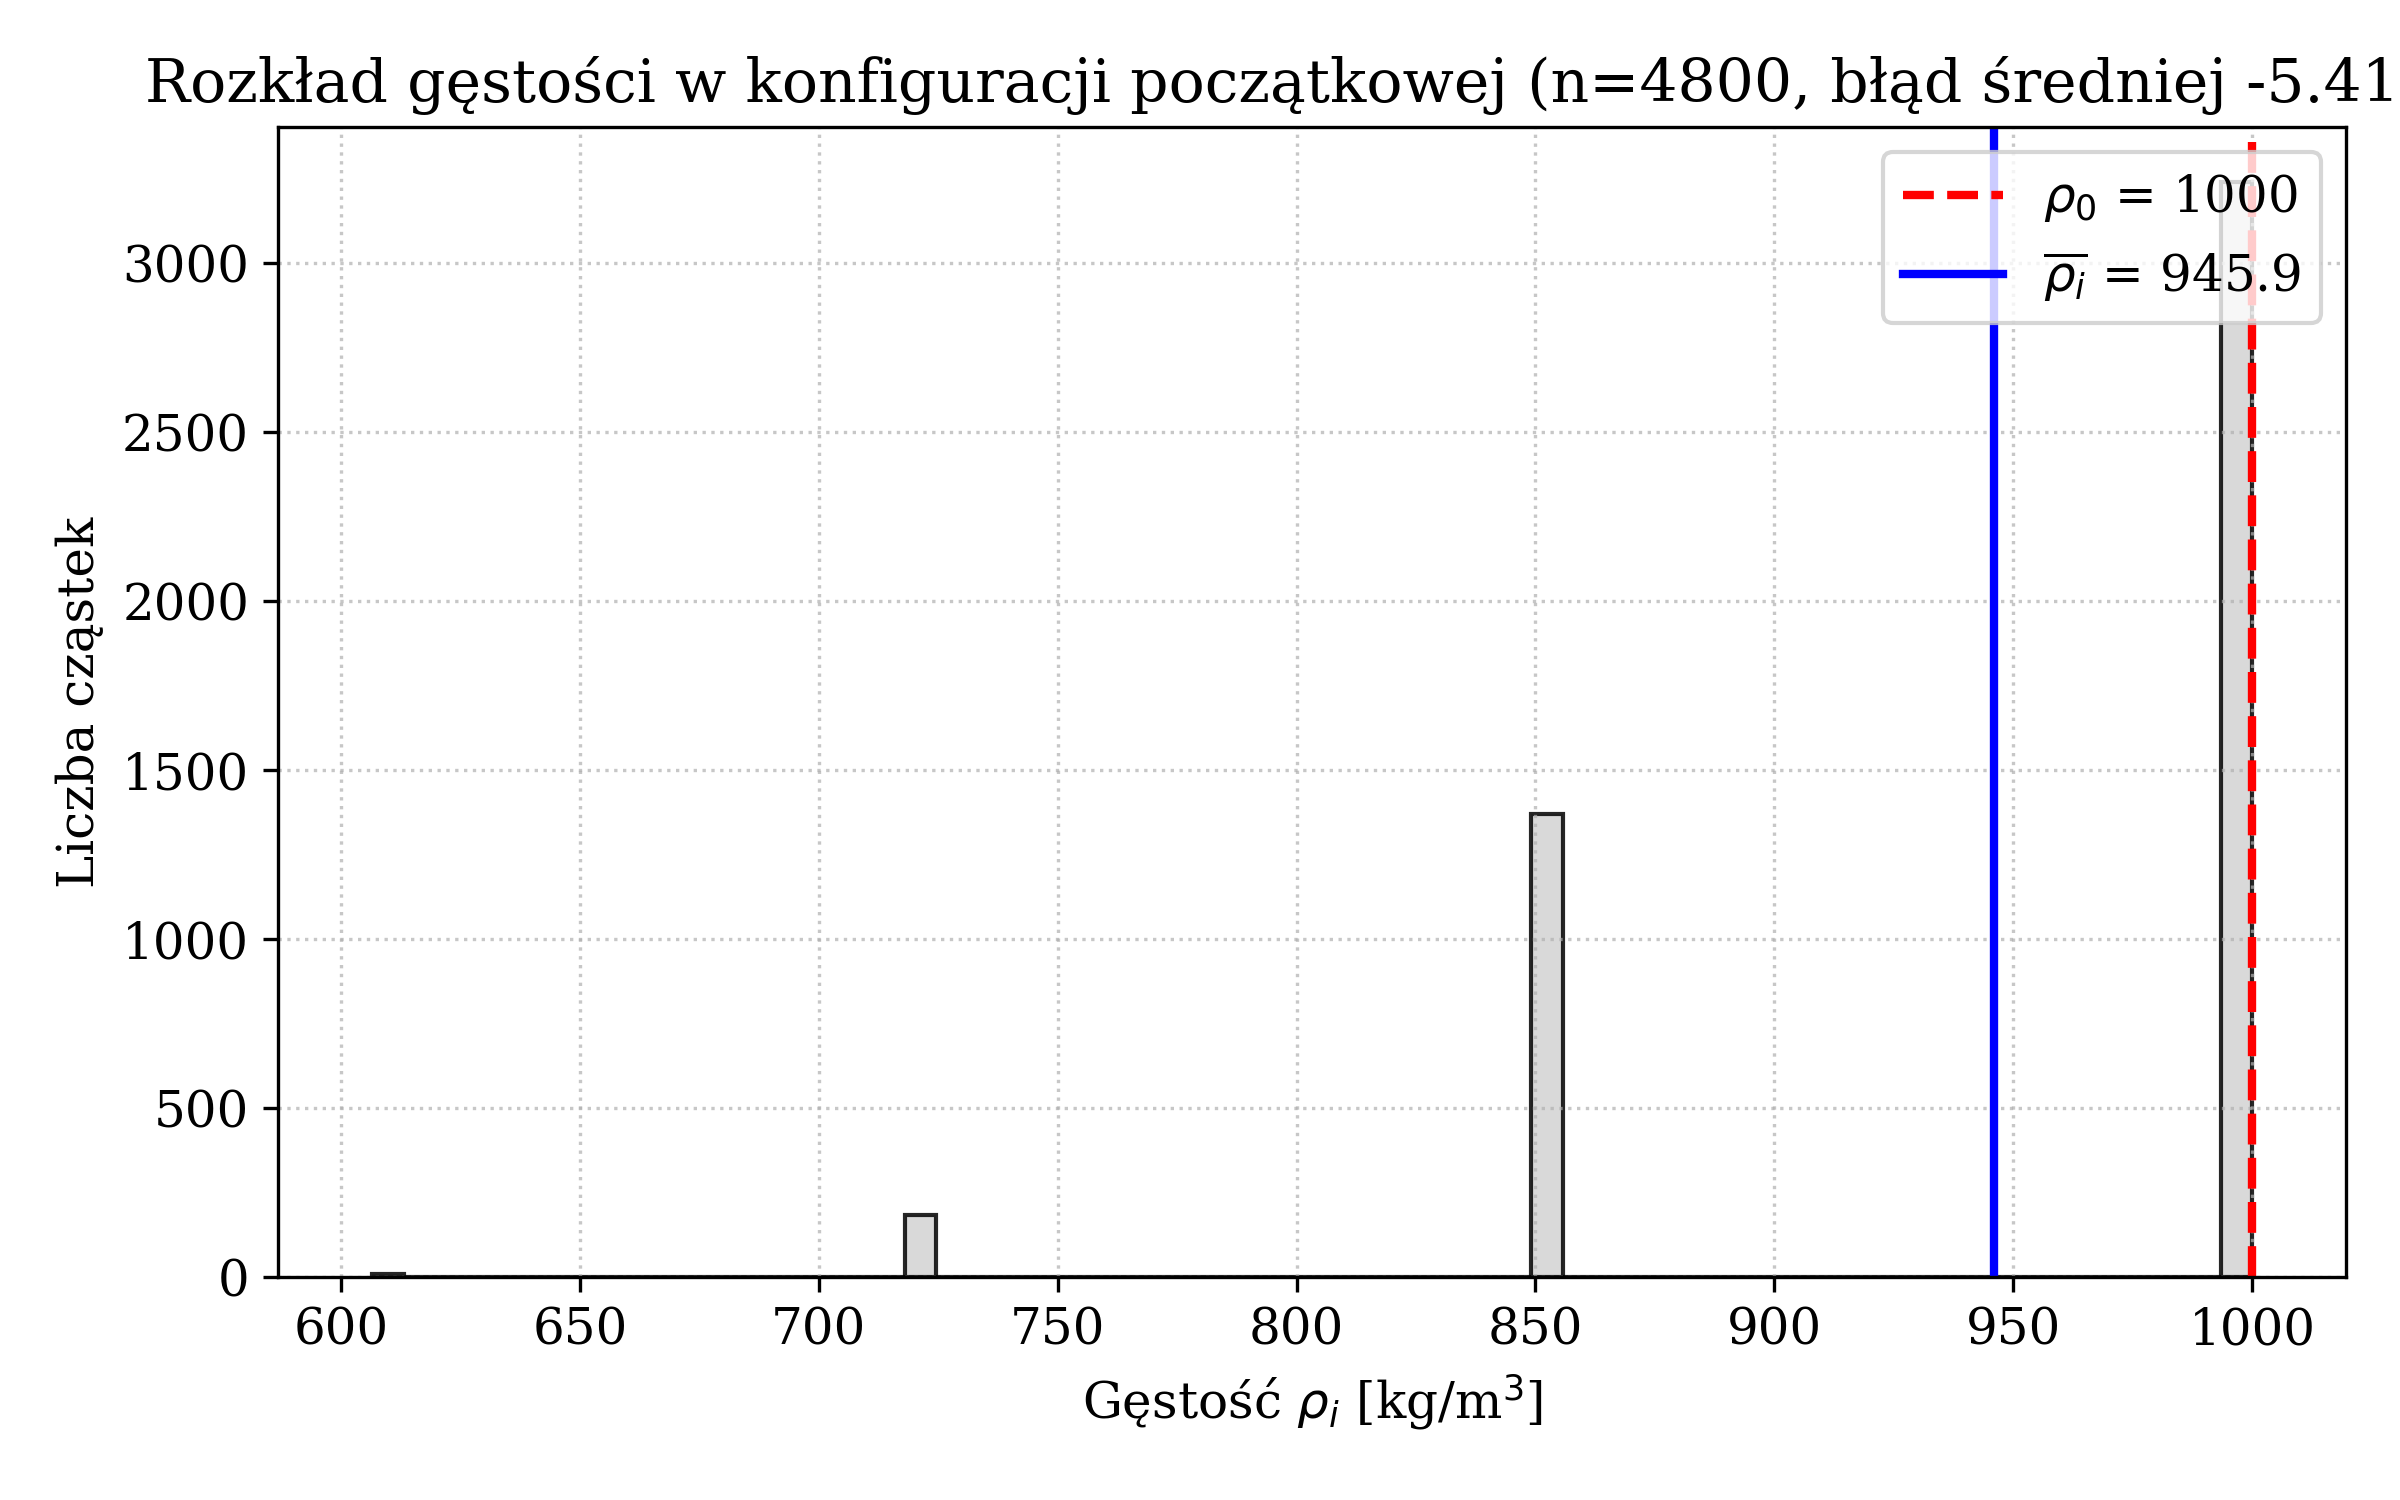
\includegraphics[width=0.85\linewidth]{figures/rest_density.png}
    \caption{Histogram gęstości w konfiguracji spoczynkowej ($n = 4800$ cząstek, bez kroku symulacji). Cząstki wewnętrzne skupiają się przy $\rho_0 = 1000~\mathrm{kg/m^3}$; cząstki przy swobodnej powierzchni wykazują deficyt będący ograniczeniem standardowego SPH bez obsługi brzegu. Źródło: opracowanie własne}
    \label{fig:rest_density}
\end{figure}

\subsection{Korekcja dywergencji}
\label{subsec:divergence_correction}

Faza korekcji dywergencji działa na prędkościach cząstek po przesunięciu ich przez solver gęstości.
Jej celem jest wyzerowanie dywergencji pola prędkości $\nabla \cdot \mathbf{v} = 0$, eliminując pozostałą składową kompresji.
Szader \texttt{divergence\_source\_term} oblicza człon źródłowy z prędkości bezpośrednio po całkowaniu ciśnień:

\begin{lstlisting}[caption={Szader \texttt{divergence\_source\_term} --- człon źródłowy solvera dywergencji},
                   label=lst:divergence_source,]
float divergence_sum = 0.0;
// dla kazdego sasiada j w promieniu h:
vec3 vel_diff = vel_i - vel_j;
divergence_sum += mass * dot(vel_diff, grad);
// koniec petli

source_terms[i] = -divergence_sum;
\end{lstlisting}

W odróżnieniu od solvera gęstości, człon źródłowy nie zawiera składnika $(\rho_0 - \rho_i)/\Delta t$ --- celem jest wyłącznie zerowanie dywergencji.
Pętla Jacobiego jest identyczna (\texttt{pressure\_force} i \texttt{pressure\_update}), natomiast szader \texttt{divergence\_integration} stosuje wynikowe ciśnienia jako korekty prędkości, nie pozycji:

\begin{lstlisting}[caption={Szader \texttt{divergence\_integration} --- całkowanie prędkości},
                   label=lst:divergence_integration,]
vec3 new_vel = vel + ap * dt;
velocities[i] = vec4(new_vel, 0.0);
\end{lstlisting}

Prawy panel Rys.~\ref{fig:convergence} ujawnia odwrotną zależność:
błąd dywergencji wzrasta wraz z liczbą iteracji i formuje symetryczne plateau od góry.
Jest to bezpośrednie sprzężenie z solverem gęstości: jedna iteracja ledwo koryguje gęstość
i nieznacznie przesuwa cząstki, pozostawiając pole prędkości prawie bezrozbieżne;
dwie i więcej iteracji skutecznie redukuje $\rho_i - \rho_0$ drogą dużych przesunięć,
które indukują proporcjonalnie silniejszą dywergencję prędkości.
Oba wykresy tworzą zatem lustrzany obraz: plateau błędu gęstości od dołu
odpowiada plateau błędu dywergencji od góry, wyznaczonemu przez skalę przesunięć
generowanych przez solver gęstości w stanie nasycenia.
Ponieważ błąd gęstości nigdy nie spada do zera z powodu deficytu jądra na brzegu,
solver gęstości stale generuje impulsy ciśnieniowe, a solver dywergencji nie ma szans
ustabilizować pola prędkości --- stąd trwałe plateau po obu stronach wykresu.

\begin{figure}[htbp]
    \centering
    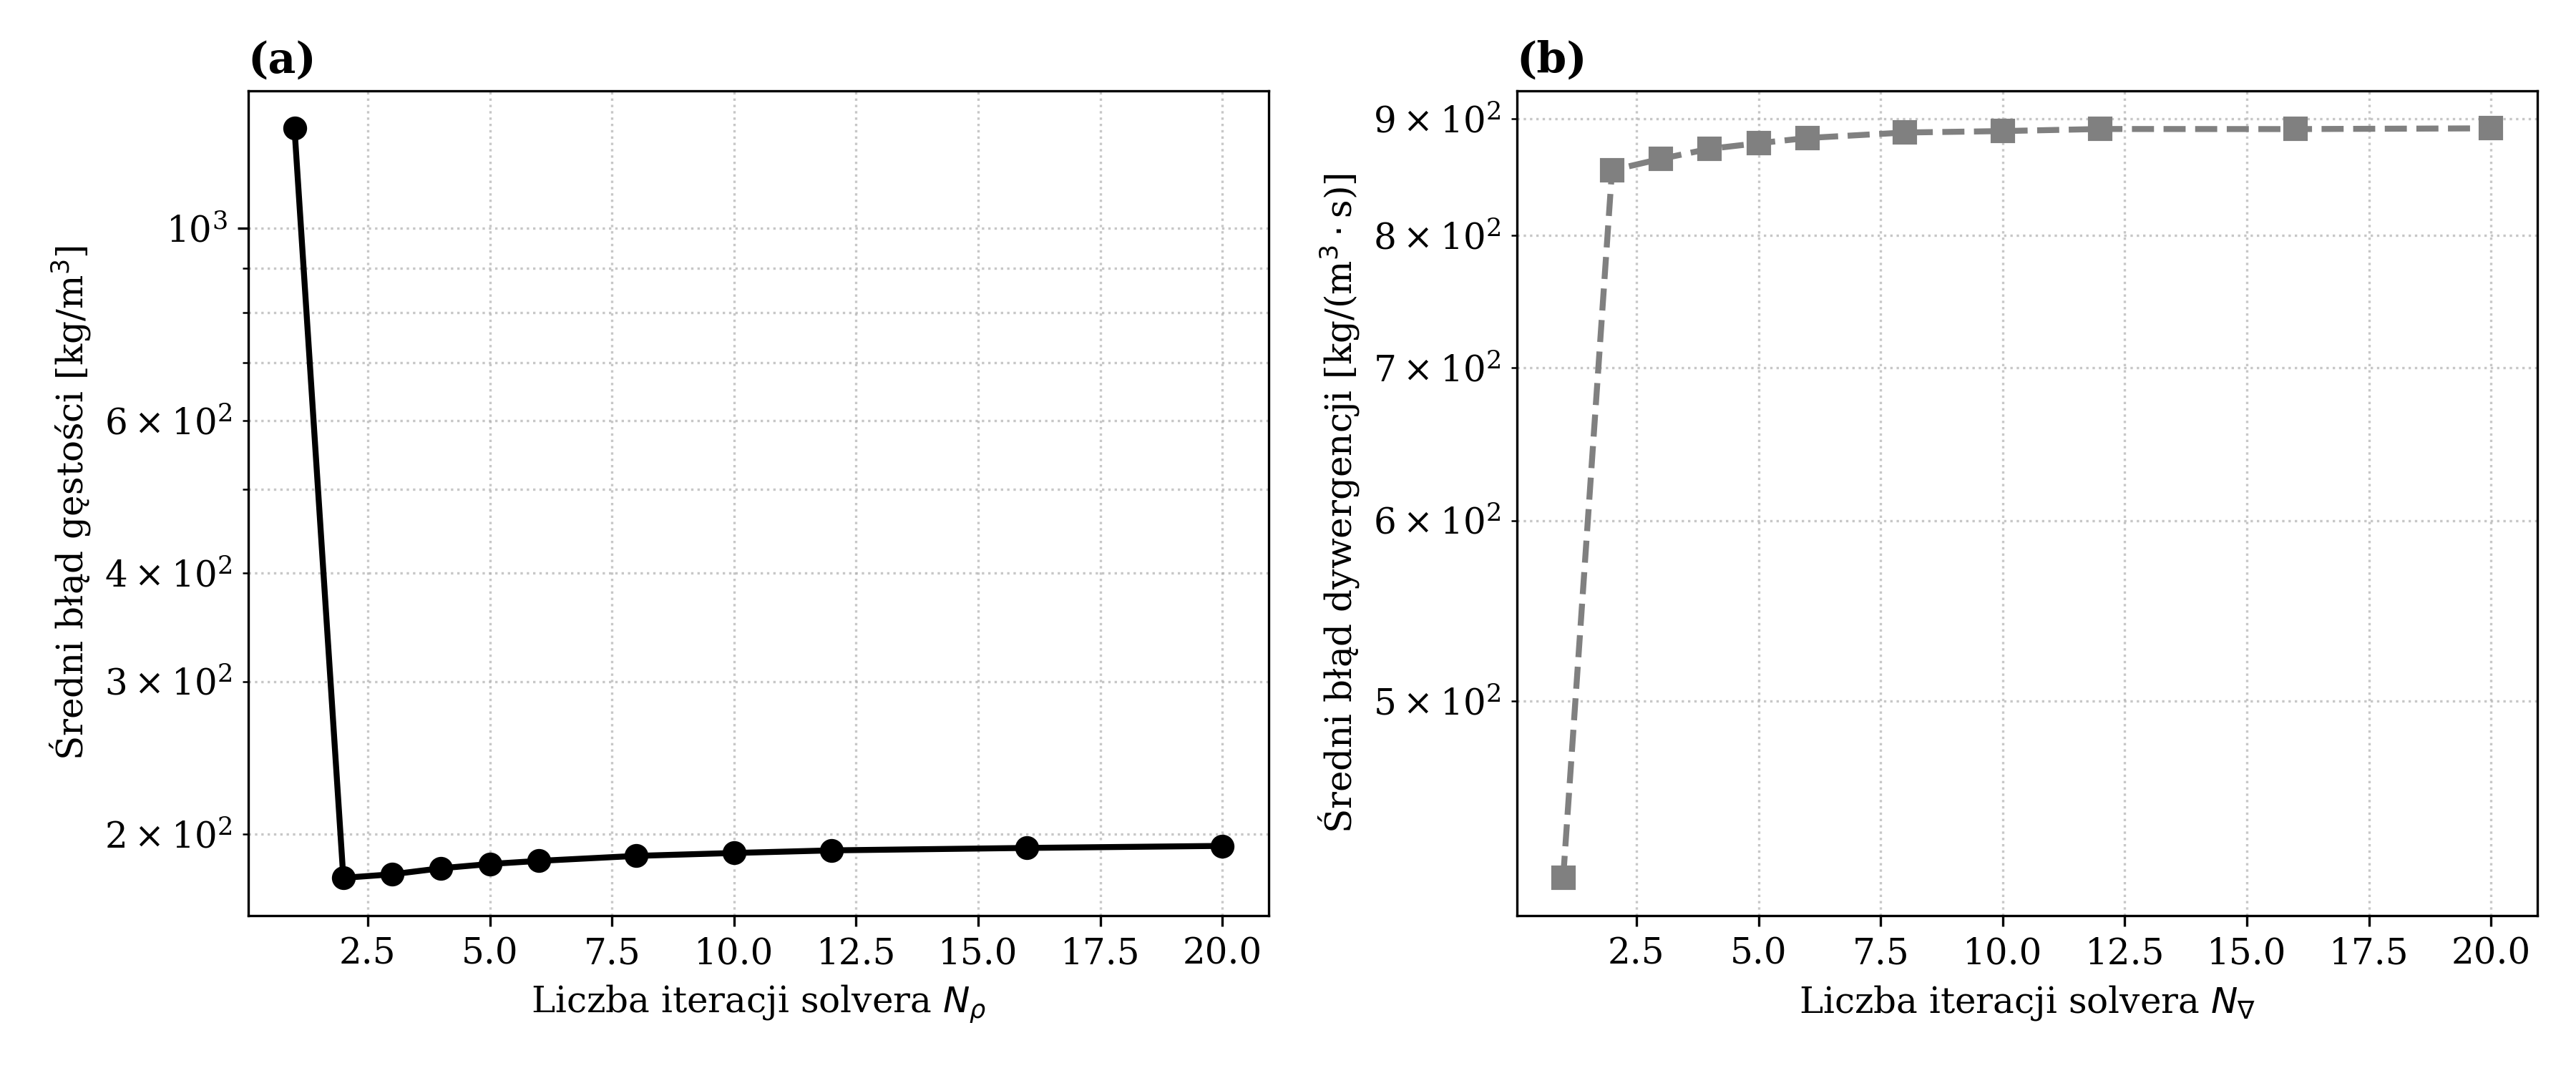
\includegraphics[width=\linewidth]{figures/convergence.png}
    \caption{Zbieżność solvera DFSPH: uśredniony błąd gęstości (lewy panel) i błąd dywergencji (prawy panel) w funkcji liczby iteracji Jacobiego. Każdy punkt to uśrednienie 40~kroków symulacji po 50~krokach rozgrzewki ($n = 4800$ cząstek). Plateau błędu gęstości wynika z deficytu jądra SPH na brzegu; plateau błędu dywergencji wynika ze sprzężenia z solverem gęstości. Źródło: opracowanie własne}
    \label{fig:convergence}
\end{figure}

\subsection{Warunek CFL i dobór \(\Delta t\)}
\label{subsec:cfl}

Dobór kroku czasowego $\Delta t$ kształtował się przez kilka etapów prób i korekt,
z których każdy ujawniał kolejną warstwę ograniczeń implementacji.

\paragraph{Etap 1 --- stały \(\Delta t\) i stała liczba iteracji.}
Pierwsza wersja symulatora operowała stałym krokiem $\Delta t = 5~\mathrm{ms}$
i czterema iteracjami Jacobiego per solver per krok symulacji.
Wynik był akceptowalny: symulacja przebiegała stabilnie przez większość czasu,
lecz sporadycznie załamywała się wskutek kumulacji błędu numerycznego.
Niska liczba klatek na sekundę skłoniła do poszukiwania optymalizacji.

\paragraph{Etap 2 --- adaptacyjny \(\Delta t\) według warunku CFL.}
Warunek CFL ogranicza krok czasowy tak,
aby cząstka nie przemieściła się o więcej niż jeden promień wygładzania $h$:
\begin{equation}
  \Delta t \leq \lambda \frac{h}{v_{\max}},
  \label{eq:cfl}
\end{equation}
gdzie $\lambda < 1$ to współczynnik bezpieczeństwa, a $v_{\max}$ to chwilowa prędkość
maksymalna odczytywana z bufora statystyk GPU (\texttt{stats\_buffer[0]}).
Gdy symulacja uspokaja się i $v_{\max}$ maleje, $\Delta t$ może wzrosnąć,
co bezpośrednio przekłada się na wyższą liczbę klatek na sekundę.
Pojawił się jednak nowy problem: większy $\Delta t$ powoduje szybsze narastanie błędu
gęstości, przez co cztery iteracje Jacobiego okazały się niewystarczające.

\paragraph{Etap 3 --- kryterium zatrzymania oparte na progu błędu.}
Naturalnym rozwinięciem było dodanie drugiego warunku zakończenia iteracji:
kontynuuj, dopóki $\overline{|\rho_i - \rho_0|} > \varepsilon$.
W założeniu solver miał wykonywać 4--5 iteracji przy spokojnej symulacji
i więcej przy gwałtownych ruchach, a rosnące $\Delta t$ kompensowało koszt
dodatkowych iteracji.
W praktyce każdy solver wykonywał sto iteracji (skonfigurowane maksimum) i nigdy
nie osiągał progu zbieżności.
Przyczyna jest dokładnie tą, którą ujawnił test zbieżności
(podrozdz.~\ref{subsec:density_correction}): deficyt jądra SPH na swobodnej
powierzchni trwale blokuje błąd gęstości na poziomie $\sim\!200~\mathrm{kg/m^3}$,
niezależnie od liczby iteracji.
Nawet milion iteracji nie obniżyłby go poniżej żadnego sensownego progu.

\paragraph{Decyzja końcowa.}
Jako kompromis powrócono do stałego $\Delta t = 5~\mathrm{ms}$ i stałej liczby
czterech iteracji per solver.
Rozwiązanie zapewnia przewidywalny koszt obliczeniowy klatki i eliminuje ryzyko
zawieszenia symulatora w nieskończonej pętli iteracyjnej.
Utrzymują się dwa znane ograniczenia: niska liczba klatek na sekundę wynikająca
z braku adaptacji kroku oraz ryzyko niestabilności numerycznej przy długich sesjach.
Oba są bezpośrednią konsekwencją braku właściwej obsługi brzegu ---
bez niej kryterium $\varepsilon$-zbieżności nie może działać poprawnie.

\begin{figure}[htbp]
  \centering
  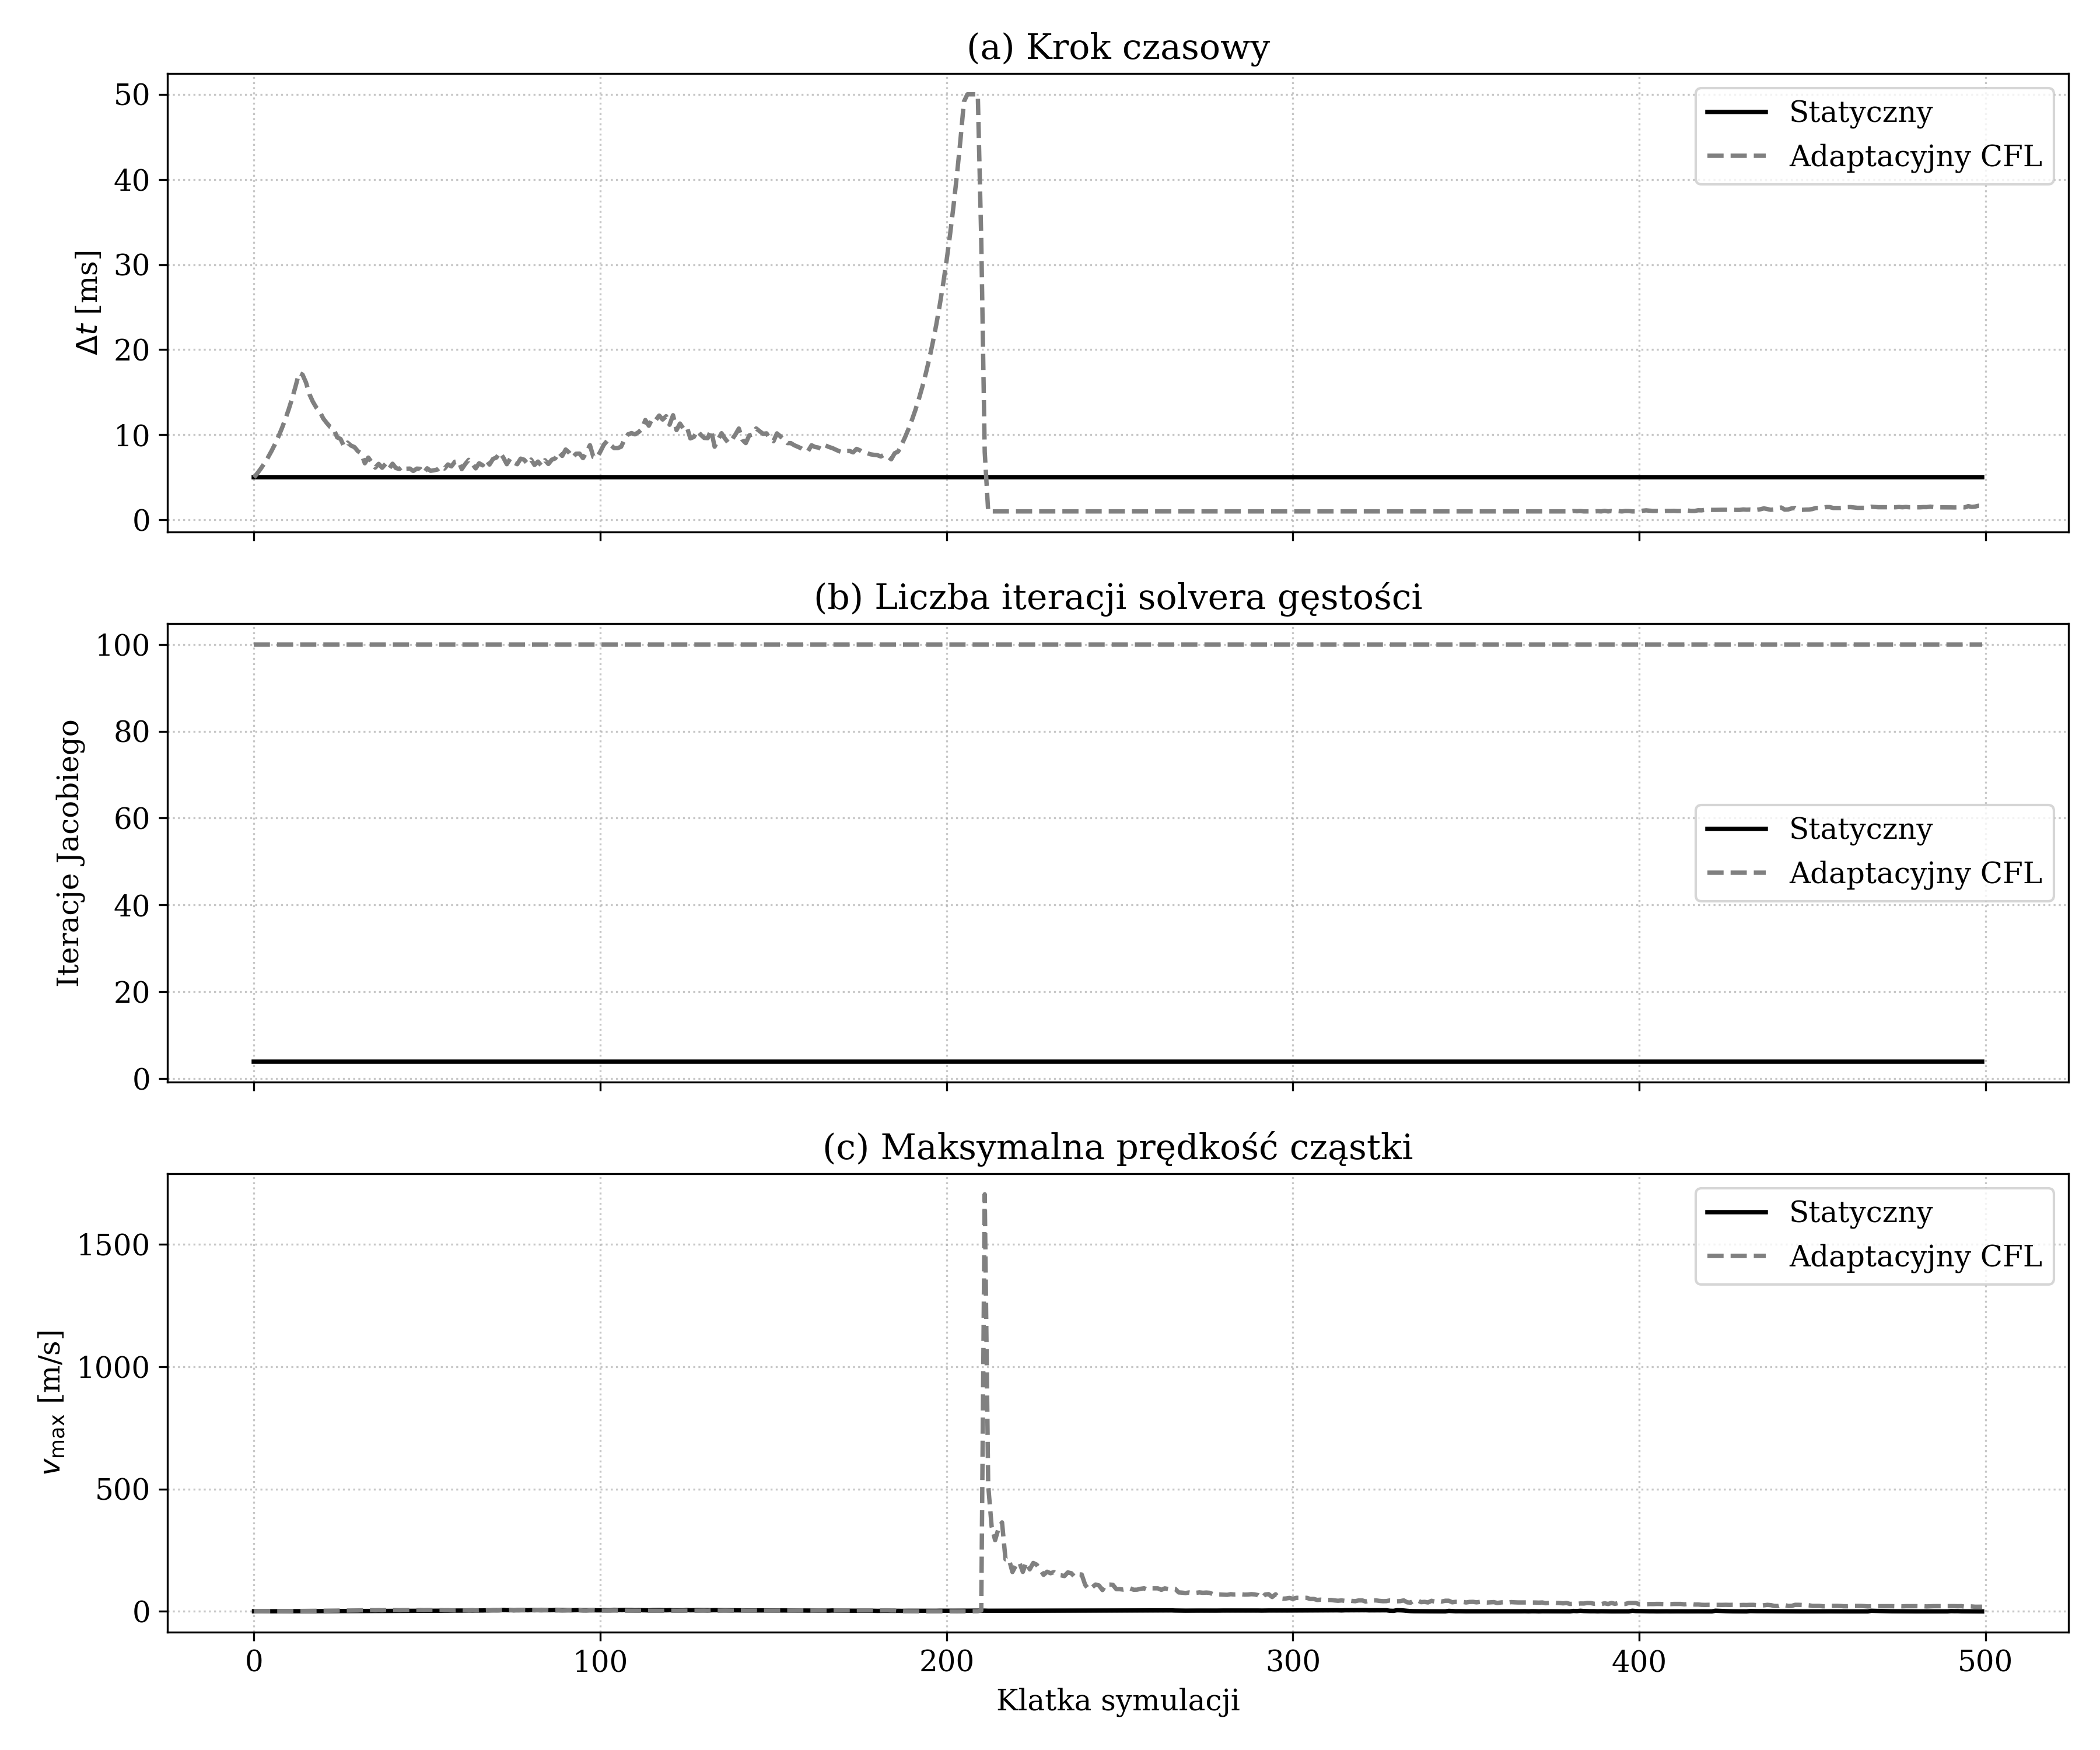
\includegraphics[width=\textwidth]{figures/cfl_comparison.png}
  \caption{Porównanie strategii statycznego $\Delta t$ (linia ciągła) i adaptacyjnego
    $\Delta t$ według warunku CFL (linia przerywana) w trakcie 500 klatek symulacji.
    \textbf{Górny panel:} krok czasowy $\Delta t$ w milisekundach.
    Wariant statyczny utrzymuje stałe $5~\mathrm{ms}$; wariant adaptacyjny rośnie
    do $50~\mathrm{ms}$ w chwilach spokoju cieczy, po czym w okolicach klatki~205
    wywołuje katastrofalną niestabilność ($v_{\max} \approx 1100~\mathrm{m/s}$)
    i opada do minimalnego $1~\mathrm{ms}$.
    \textbf{Środkowy panel:} liczba iteracji solvera Jacobiego.
    Wariant statyczny utrzymuje stałe cztery iteracje; wariant adaptacyjny
    osiąga limit 100 iteracji w każdej klatce bez wyjątku, ponieważ próg
    $\varepsilon$ nigdy nie jest spełniony.
    \textbf{Dolny panel:} maksymalna prędkość cząstki $v_{\max}$.
    Po eksplozji prędkość stabilizuje się na poziomie $20$--$40~\mathrm{m/s}$,
    co wskazuje na stan uszkodzonej symulacji.\\
    Źródło: opracowanie własne}
  \label{fig:cfl_comparison}
\end{figure}

% ------------------------------------------------------------
\section{Siły fizyczne}
\label{sec:forces}

Podrozdział ten opisuje implementację dwóch mechanizmów siłowych działających
na cząsteczki poza solverem DFSPH: wygładzenia prędkości metodą XSPH oraz
odpowiedzi na kolizje z granicą domeny.
Podstawy teoretyczne obu metod omówiono w podrozdziale~\ref{sec:physical_models_theory};
poniżej skupiono się na konkretnych wyborach implementacyjnych i stałych
liczbowych przyjętych w kodzie.

\subsection{Lepkość XSPH}
\label{subsec:xsph}

Wygładzenie prędkości XSPH realizowane jest w shaderze \texttt{viscosity}.
Poniższy listing przedstawia rdzeń obliczeń --- pętlę po sąsiadach
i końcową aktualizację prędkości:

\begin{lstlisting}[caption={Rdzeń shadera \texttt{viscosity} --- korekcja XSPH i grawitacja},
                   label=lst:xsph,]
vec3 sum_viscosity = vec3(0.0);
// dla kazdego sasiada j w promieniu h:
vec3 vel_diff = velocities[j].xyz - velocities[i].xyz;
sum_viscosity += mass / densities[j] * vel_diff * kernel_w(r, h);
// koniec petli

vec3 vel_visco = velocities[i].xyz
               + sim_params.viscosity * sum_viscosity;
new_velocities[i] = vec4(vel_visco + sim_params.gravity.xyz
                                   * sim_params.dt, 0.0);
\end{lstlisting}

Bezwymiarowy współczynnik wygładzenia $\nu$ przechowywany jest w polu
\texttt{viscosity} struktury \texttt{SimulationParams}.
Wartość $\nu = 0{,}15$ dobrano empirycznie: wartości poniżej $0{,}05$
dopuszczają widoczne przenikanie cząsteczek przy zderzeniach,
powyżej $0{,}4$ nadmiernie tłumią ruch i spowalniają opadanie.
Parametr jest dostępny w czasie wykonania przez suwak interfejsu egui
bez potrzeby ponownej kompilacji shaderów.

Grawitacja dodawana jest w tej samej przepustce tuż po korekcji XSPH,
co eliminuje oddzielny dispatch i jedno przejście przez bufor prędkości.
Wynik trafia do bufora \texttt{new\_velocities}; zapis i odczyt dotyczą
różnych buforów, więc kolejność wątków nie wpływa na wynik.

\subsection{Obsługa kolizji}
\label{subsec:collision}

Reakcja na kolizję z ścianą odbywa się na końcu shadera
\texttt{pressure\_integration}, bezpośrednio po całkowaniu Eulera.
Listing~\ref{lst:collision} pokazuje obsługę jednej ściany (dolna granica
osi~$y$); pozostałe pięć ścian realizowane są analogicznie:

\begin{lstlisting}[caption={Fragment \texttt{pressure\_integration} --- odbicie od dolnej sciany},
                   label=lst:collision,]
float restitution = 0.5;
float friction    = 0.95;
float eps         = 0.001;

if (new_pos.y < min_b.y + r) {
    new_pos.y  = min_b.y + r + eps;
    new_vel.y *= -restitution;
    new_vel.xz *= friction;
}
\end{lstlisting}

Stała \texttt{eps} przesuwa cząsteczkę o $1~\mathrm{mm}$ ponad granicę,
zapobiegając wielokrotnemu wyzwalaniu warunku w kolejnych krokach.
Współczynnik sprężystości $e = 0{,}5$ pochłania połowę energii normalnej
przy każdym odbiciu; tarcie styczne $f = 0{,}95$ nieznacznie tłumi
ruch równoległy do ściany, nie zatrzymując cząsteczki całkowicie.

Podejście to nie koryguje deficytu jądra przy brzegu omówionego
w~podrozdz.~\ref{subsec:divergence_correction}, lecz skutecznie
zapobiega ucieczce cząsteczek z domeny i jest wystarczające dla
wizualnie wiarygodnych scen zamkniętych.

% ------------------------------------------------------------
\section{Wizualizacja}
\label{sec:visualization}

Potok wizualizacji przekształca listę pozycji cząsteczek w gotowy kolor piksela
w trzech etapach: splatowanie gęstości do trójwymiarowej tekstury, przemarsz promienia
przez tę teksturę do znalezienia powierzchni, oraz model optyczny łączący odbicie,
załamanie, absorpcję i rozproszenie podpowierzchniowe.
Podstawy teoretyczne wszystkich etapów omówiono w podrozdziale~\ref{sec:visualization_pipeline_theory};
poniżej przedstawiono konkretne stałe i fragmenty kodu z implementacji.

\subsection{Splatowanie gęstości do tekstury 3D}
\label{subsec:density_splat}

Shader \texttt{splat\_density} dla każdej cząsteczki wyznacza woksel centralny,
a następnie iteruje po sześcianie $\pm 8$ wokseli i atomowo dodaje wkład do tekstury:

\begin{lstlisting}[caption={Shader \texttt{splat\_density} --- waga woksela i zapis atomowy},
                   label=lst:splat,]
int radius = 8;
\ dla kazdego woksela (x,y,z) w szescianie [-radius, radius]^3:
float dist   = length(vec3(x, y, z));
if (dist < float(radius)) {
    float x_norm = dist / float(radius);
    float weight = (1.0 - x_norm * x_norm);
    weight = weight * weight * weight;

    uint contrib = uint(weight * 200.0);
    imageAtomicAdd(density_grid, currentVoxel, contrib);
}
\end{lstlisting}

Waga jest gładkim wielomianem $(1-q^2)^3$ tożsamym z~eq.~\ref{eq:splat_weight}.
Mnożnik $200$ skaluje wartość do zakresu liczby całkowitej bez utraty precyzji;
woksele powietrza osiągają wartości bliskie zeru, woksele wewnątrz cieczy --- rzędu
setek.
Tekstura ma format \texttt{R32Uint}; stała \texttt{DENSITY\_OFFSET = 300} odejmowana
jest przy odczycie w shaderze fragmentów, eliminując szum tła bez progowania binarnego.

\subsection{Ray Marching}
\label{subsec:raymarching}

Pętla przemarszu w \texttt{raymarch} składa się z trzech faz: testu AABB,
grubego kroku oraz bisekcji refinementu.

\paragraph{Test AABB i krok gruby.}
Przed wejściem w pętlę funkcja \texttt{intersectAABB} wyznacza analitycznie
przedział $[t_{\min}, t_{\max}]$ wejścia i wyjścia promienia z domeny;
promienie chybiające domenę odrzucane są natychmiast instrukcją \texttt{discard}.

\begin{lstlisting}[caption={Fragment \texttt{raymarch} --- test AABB i petla przemarszu},
                   label=lst:march_loop,]
const int   MAX_STEPS = 96;
const float STEP_SIZE = 0.007;

vec2 tHit = intersectAABB(rayOrigin, rayDir, boxMin, boxMax);
if (tHit.x > tHit.y || tHit.y < 0.0) discard;

float stepWorld = STEP_SIZE
                * max(max(boxScale.x, boxScale.y), boxScale.z);
float tCurrent  = max(tHit.x, 0.0);

for (int i = 0; i < MAX_STEPS; i++) {
    if (tCurrent > tHit.y) break;
    if (getDensity(rayOrigin + rayDir * tCurrent, ...) > 0.01) {
        hit = true; break;
    }
    tCurrent += stepWorld;
}
if (!hit) discard;
\end{lstlisting}

Krok \texttt{stepWorld} skalowany jest rozmiarem sceny, dzięki czemu ta sama stała
\texttt{STEP\_SIZE} działa poprawnie niezależnie od proporcji domeny.
Promienie, które nie trafią w żaden woksel powyżej progu w 96 krokach, są odrzucane
instrukcją \texttt{discard} jeszcze na etapie shadera fragmentów.

\paragraph{Bisekcja i normalna.}
Po wykryciu pierwszego przekroczenia progu przedział $[t_0, t_1]$ zawężany
jest ośmiokrotną bisekcją, a normalna wyznaczana jest różnicami skończonymi
na polu gęstości.

\begin{lstlisting}[caption={Fragment \texttt{raymarch.frag} --- bisekcja i normalna},
                   label=lst:bisect,]
float t0 = tCurrent - stepWorld, t1 = tCurrent;
for (int i = 0; i < 8; i++) {
    float m = (t0 + t1) * 0.5;
    if (getDensity(rayOrigin + rayDir * m, ...) > 0.01)
        t1 = m;
    else
        t0 = m;
}
vec3 surfacePos = rayOrigin + rayDir * t1;
vec3 N = -calcNormal(surfacePos, boxMin, boxMax);
if (dot(N, N) < 0.5) N = vec3(0.0, 1.0, 0.0);
\end{lstlisting}

Osiem iteracji bisekcji zawęża punkt trafiania do dokładności
$\Delta t / 2^8 \approx 0{,}4\%$ kroku bez zmniejszania globalnego
\texttt{STEP\_SIZE}.
Normalna wyznaczana jest sześcioma próbkami pola gęstości metodą różnic skończonych
(\texttt{eps = 0.018}); warunek \texttt{dot(N,N) < 0.5} zastępuje normalną wektorem
pionowym w miejscach, gdzie gradient zanika (płaskie dno).

\paragraph{Interpolacja trójliniowa.}
Próbkowanie tekstury \texttt{R32Uint} realizowane jest ręcznie, ponieważ format
całkowitoliczbowy nie obsługuje sprzętowej interpolacji:

\begin{lstlisting}[caption={Funkcja \texttt{getDensity} --- interpolacja trojliniowa},
                   label=lst:trilinear,]
vec3 gridPos = uvw * vec3(sim_params.grid_res.xyz) - 0.5;
ivec3 iobase = ivec3(floor(gridPos));
vec3  f      = fract(gridPos);
\ 8 wywolan texelFetch dla wierzcholkow kostki (v000..v111)
float v0 = mix(mix(v000, v100, f.x), mix(v010, v110, f.x), f.y);
float v1 = mix(mix(v001, v101, f.x), mix(v011, v111, f.x), f.y);
return max(0.0, (mix(v0, v1, f.z) - DENSITY_OFFSET) 
                    * DENSITY_MULTIPLIER);
\end{lstlisting}

Odjęcie \texttt{DENSITY\_OFFSET = 300} zeruje szum tła; \texttt{max(0.0, ...)}
zapobiega ujemnym wartościom gęstości w wokselach powietrza.

\subsection{Model oświetlenia}
\label{subsec:shading}

Cały model optyczny zamknięty jest w funkcji \texttt{main()} shadera
\texttt{raymarch.frag} i wykonywany po znalezieniu punktu powierzchni.

\paragraph{Fresnel, odbicie i załamanie.}
Współczynnik odbicia $F_0$ wyznaczany jest ze wzoru Fresnela, a promienie
odbitego i załamanego kierunku próbkują skybox:

\begin{lstlisting}[caption={Fragment \texttt{raymarch.frag} --- Fresnel, odbicie, zalamania},
                   label=lst:fresnel,]
const float IOR_WATER = 1.333;
const float IOR_AIR   = 1.0;

float F0 = pow((IOR_AIR - IOR_WATER) / (IOR_AIR + IOR_WATER), 2.0);
float F  = fresnel(NdotV, F0);  // przyblizenie Schlicka

vec3 reflDir    = reflect(rayDir, N);
vec3 reflection = sampleSkybox(reflDir);
reflection += SUN_COLOR * clamp(ggxD(NdotH, 0.04) 
                * NdotL * 0.15, 0.0, 3.0);

vec3 refrDir    = refract(rayDir, N, IOR_AIR / IOR_WATER);
if (dot(refrDir, refrDir) < 0.01) refrDir = rayDir;
vec3 background = sampleSkybox(normalize(refrDir));
\end{lstlisting}

Wartość $F_0 \approx 0{,}02$ obliczana jest ze wzoru Fresnela dla granicy
woda--powietrze; przy kącie ślizgowym wzrasta do jedności zgodnie z przybliżeniem
Schlicka.
W przypadku całkowitego wewnętrznego odbicia \texttt{refract} zwraca wektor zerowy;
kierunek zastępowany jest wówczas oryginalnym promieniem.

\paragraph{Absorpcja, SSS i piana.}
Grubość cieczy wzdłuż promienia steruje absorpcją Beer-Lamberta,
rozproszeniem podpowierzchniowym i maską piany; wynik składany jest
operatorem Reinharda do zakresu $[0,\,1]$:

\begin{lstlisting}[caption={Fragment \texttt{raymarch.frag} --- absorpcja, SSS, piana, tonowanie},
                   label=lst:sss,]
const vec3 ABSORPTION_COEFF = vec3(0.45, 0.085, 0.025);
const vec3 SCATTER_COLOR    = vec3(0.04, 0.18,  0.28);

float thickness  = calcThickness(
    surfacePos, 
    rayDir, 
    tHit.y - t1, ...);
vec3  absorption = exp(-ABSORPTION_COEFF * thickness * 8.0);

float sssWrapped = max(0.0, dot(N,  L) * 0.5 + 0.5);
float sssBack    = max(0.0, dot(-N, L));
float sssFactor  = (sssWrapped * 0.6 + sssBack * 0.4)
                 * (1.0 - exp(-thickness * 3.0));
vec3 sss = SCATTER_COLOR * SUN_COLOR * sssFactor * SCATTER_STRENGTH;

float foamMask = smoothstep(0.0, 0.3, thickness)
               * smoothstep(0.5, 0.95, N.y);

vec3 refracted  = background * absorption + sss;
vec3 waterColor = mix(refracted, reflection, F);
waterColor = mix(
    waterColor, 
    FOAM_COLOR * (NdotL * 0.7 + 0.3), 
    foamMask * 0.7);
waterColor = waterColor / (waterColor + vec3(1.0));
\end{lstlisting}

Grubość \texttt{thickness} mierzona jest osobnym przelotem 32 próbek od punktu
powierzchni do tylnej ściany AABB (\texttt{calcThickness}).
Silna absorpcja kanału czerwonego ($\mu_R = 0{,}45$) przy słabej niebieskiego
($\mu_B = 0{,}025$) daje wodzie charakterystyczną niebieskozieloną barwę.
Maska piany aktywuje się tam, gdzie normalna jest prawie pionowa
(\texttt{N.y} bliskie $1$) i ciecz jest cienka --- naśladując bąble
na grzbietach fali.
Ostatnia linia to operator Reinharda sprowadzający zakres HDR do $[0,\,1]$.

\subsection{Środowisko HDRI}
\label{subsec:hdri}

Otoczenie sceny reprezentuje sferyczna mapa w formacie równokątnym ładowana
z pliku \texttt{.exr} przy starcie aplikacji.
Funkcja \texttt{sampleSkybox} przelicza dowolny kierunek przestrzenny na
współrzędne UV tej tekstury:

\begin{lstlisting}[caption={Funkcja \texttt{sampleSkybox} --- odwzorowanie rownokatne},
                   label=lst:skybox,]
vec3 sampleSkybox(vec3 dir) {
    dir = normalize(dir);
    vec2 uv = vec2(atan(dir.z, dir.x) * 0.15915 + 0.5,
                   asin(clamp(dir.y, -1.0, 1.0)) * 0.31831 + 0.5);
    return texture(skyboxTex, uv).rgb;
}
\end{lstlisting}

Stałe $\tfrac{1}{2\pi} \approx 0{,}15915$ i $\tfrac{1}{\pi} \approx 0{,}31831$
normalizują kąty azymutowy i elewacji do przedziału $[0,\,1]$.
Ta sama funkcja wywoływana jest zarówno dla promienia odbitego, jak i załamanego,
zapewniając spójność oświetlenia między powierzchnią cieczy a tłem.
Skybox renderowany jest osobnym shaderem \texttt{sky.frag} na sferze
o promieniu $500$ ze odwróconymi normalami, tak by kamera zawsze znajdowała
się w jej środku.


% 6. Підсумок
\chapter*{Podsumowanie}
\addcontentsline{toc}{chapter}{Podsumowanie}
\chaptermark{Podsumowanie}
Celem niniejszej pracy było zaprojektowanie i~zaimplementowanie interaktywnego
silnika symulacji cieczy, wykonującego pełny potok obliczeniowy --- od dynamiki
cząstek po gotowy obraz --- w~czasie rzeczywistym na procesorze graficznym.
Punkt wyjścia stanowiła analiza eulerowskiego i~lagrange'owskiego opisu ruchu
płynów oraz matematyczne sformułowanie metody SPH wraz z~wariantem DFSPH,
wymuszającym nieściśliwość cieczy przez dwuetapową korekcję gęstości
i~dywergencji. Tak zdefiniowane podstawy teoretyczne przełożono na implementację
w~języku Rust z~wykorzystaniem API Vulkan, a~każdą istotną decyzję projektową
uzasadniono analizą strukturalną lub bezpośrednim pomiarem.

W~ramach pracy zrealizowano następujące zadania:
\begin{itemize}
    \item dokonano przeglądu istniejących rozwiązań symulacji cieczy
          (Blender, Unreal Engine~5, SPlisHSPlasH) i~wyznaczono na ich tle
          miejsce własnego systemu: czysto cząsteczkowej implementacji DFSPH
          wykonywanej w~całości na GPU;
    \item zaimplementowano kompletny solver DFSPH jako zestaw jedenastu potoków
          obliczeniowych, obejmujących wyznaczanie gęstości i~współczynnika
          $\alpha$, iteracyjne pętle korekcji ciśnienia oraz całkowanie ruchu
          cząstek;
    \item opracowano wyszukiwanie sąsiedztwa oparte na haszowaniu przestrzennym
          z~reorganizacją buforów, zapewniające stały czas zapytania
          i~skoalescowane odczyty pamięci GPU;
    \item zaimplementowano i~porównano ilościowo dwa algorytmy sortowania
          na GPU --- sortowanie bitoniczne i~pozycyjne --- wykazując niemal
          sześciokrotną przewagę tego drugiego w~pełnym potoku symulacji;
    \item zaprojektowano organizację danych SOA z~podwójnym buforowaniem pozycji
          i~prędkości, strukturalnie eliminującą wyścigi danych między wątkami
          GPU;
    \item zbudowano wolumetryczny potok wizualizacji: splatting gęstości
          do tekstury trójwymiarowej, przemarsz promienia z~bisekcją oraz model
          optyczny wody łączący efekt Fresnela, absorpcję Beer-Lamberta,
          rozproszenie podpowierzchniowe, odbłysk GGX i~oświetlenie panoramą
          HDRI;
    \item przeprowadzono analizę zbieżności obu solverów oraz eksperymenty
          z~adaptacyjnym krokiem czasowym według warunku CFL, dokumentując
          źródła ich ograniczeń;
    \item udostępniono interaktywny panel konfiguracji umożliwiający modyfikację
          parametrów fizycznych i~wizualnych w~trakcie działania symulacji.
\end{itemize}

Wynikiem pracy jest działający symulator zdolny do stabilnej animacji dziesiątek
tysięcy cząstek w~czasie rzeczywistym, wraz z~zestawem narzędzi diagnostycznych
i~pomiarowych. Przeprowadzone testy ujawniły zarazem najważniejsze ograniczenie
przyjętego modelu: brak właściwej obsługi brzegu powoduje trwały deficyt
gęstości przy swobodnej powierzchni, który blokuje kryterium zbieżności solvera
i~uniemożliwia bezpieczne stosowanie adaptacyjnego kroku czasowego
(podrozdz.~\ref{subsec:cfl}). Świadomy powrót do stałego $\Delta t$ i~stałej
liczby iteracji stanowi udokumentowany kompromis między stabilnością
a~wydajnością.

Niniejsza praca koncentrowała się przede wszystkim na warstwie fizycznej
symulacji; ta orientacja wyznacza naturalne kierunki dalszego rozwoju systemu.

\begin{itemize}
    \item \textbf{Uzupełnienie modelu fizycznego.} Pierwszym krokiem powinna być
          obsługa brzegu za pomocą cząstek-duchów lub stałych warstw cząstek
          brzegowych~\cite{schechter2012ghost}, która usunęłaby deficyt jądra
          przy powierzchni i~odblokowała zarówno kryterium
          $\varepsilon$-zbieżności, jak i~adaptacyjny warunek CFL. Kolejnym
          naturalnym rozszerzeniem jest implementacja napięcia powierzchniowego,
          otwierająca drogę do zjawisk kapilarnych, formowania kropel
          i~realistycznego zachowania cienkich warstw cieczy.
    \item \textbf{Rozbudowa warstwy wizualizacji.} Ponieważ wizualizacja pełniła
        w~pracy rolę służebną wobec fizyki, pozostaje tu szerokie pole
        eksperymentów. Obejmują one jawną rekonstrukcję powierzchni metodą
        maszerujących sześcianów (ang.~\textit{marching cubes}), techniki
        renderowania w~przestrzeni ekranu oraz cząstki wtórne piany i~rozbryzgów.
        Dodatkowo, wdrożenie sprzętowego śledzenia promieni poprzez rozszerzenie
        \texttt{VK\_KHR\_ray\_tracing\_pipeline} pozwoliłoby na uzyskanie fizycznie
        poprawnych kaustyk i~wielokrotnych odbić światła w~objętości cieczy.
    \item \textbf{Techniki optymalizacji.} Obiecującym kierunkiem są
          skompresowane listy sąsiedztwa~\cite{band2019compressed}, których
          pełna realizacja na GPU pozostaje otwartym problemem badawczym,
          a~ponadto adaptacyjna rozdzielczość cząstek zagęszczająca symulację
          wyłącznie w~obszarach istotnych wizualnie oraz głębsze wykorzystanie
          pamięci dzielonej i~operacji podgrupowych
          (ang.~\textit{subgroup operations}) w~shaderach solvera.
    \item \textbf{Integracja z~ekosystemem.} Silnik może zostać przekształcony
          w~bibliotekę wielokrotnego użytku lub rozwinięty w~stronę
          pełnoprawnego silnika aplikacji interaktywnych; alternatywą jest
          opakowanie go we wtyczkę do istniejącego środowiska, analogicznie
          do roli, jaką NiagaraFluids pełni w~Unreal Engine~5. Krokiem
          poprzedzającym byłoby usunięcie zależności od platformy Windows
          i~udostępnienie wersji dla systemów Linux i~macOS.
    \item \textbf{Metody oparte na danych.} Odrębną perspektywę otwiera
          częściowe lub całkowite zastąpienie obliczeń fizycznych modelami
          statystycznymi i~sieciami neuronowymi: aproksymacja kroku solvera
          modelem nauczonym na danych z~symulacji referencyjnych, generowanie
          detali wysokiej częstotliwości na podstawie zgrubnej symulacji
          o~małej liczbie cząstek czy statystyczna analiza pól prędkości
          i~gęstości pozwalająca przewidywać zachowanie cieczy bez jawnego
          rozwiązywania równań ruchu.
\end{itemize}

Przeprowadzone prace potwierdzają, że połączenie języka Rust i~API Vulkan
stanowi dojrzały fundament dla wysokowydajnych symulacji fizycznych: statyczne
gwarancje kompilatora wyeliminowały całą klasę błędów zarządzania pamięcią,
a~jawna kontrola nad procesorem graficznym pozwoliła przenieść na niego
kompletny potok obliczeniowy. Powstały system --- wraz z~opisanymi w~pracy
pomiarami, diagnozami i~zidentyfikowanymi ograniczeniami --- może służyć jako
platforma odniesienia i~punkt wyjścia dla wymienionych wyżej kierunków badań.

\cleardoublepage

\cleardoublepage
\addcontentsline{toc}{chapter}{Spis rysunków}
\listoffigures

\cleardoublepage
\addcontentsline{toc}{chapter}{Bibliografia}
\bibliography{bibliography}

\end{document}